\documentclass[10pt]{article}
\usepackage[T1]{fontenc}
\usepackage[utf8]{inputenc}
\usepackage{lmodern}
\usepackage[margin=0.7in]{geometry}
\usepackage{amsmath,amssymb}
\usepackage{microtype}
\usepackage{enumitem}
\usepackage{booktabs}
\usepackage{graphicx}
\usepackage{placeins}
\usepackage[font=small,labelfont=bf]{caption}
\usepackage[dvipsnames]{xcolor}
\usepackage[backend=bibtex,style=authoryear,natbib=true,maxcitenames=2,maxbibnames=4,minbibnames=3,uniquelist=false,uniquename=false,giveninits=true,doi=false,isbn=false,url=false,eprint=false]{biblatex}
\addbibresource{refs.bib}
\usepackage[colorlinks=true,linkcolor=MidnightBlue,citecolor=MidnightBlue,urlcolor=MidnightBlue]{hyperref}
\usepackage[capitalise,nameinlink]{cleveref}
\setlength{\parskip}{3pt}
\setlength{\parindent}{0pt}
\makeatletter
\renewcommand\paragraph{\@startsection{paragraph}{4}{\z@}{1.2ex \@plus .4ex \@minus .2ex}{-1em}{\normalfont\normalsize\bfseries}}
\makeatother
\setlist{nosep,leftmargin=*}

%% Placeholders for results (rendered in red).
\DeclareRobustCommand{\todo}[1]{\textcolor{red}{[TODO: #1]}}
\newcommand{\extra}{\textsuperscript{\dag}}  % added after the project plan
\DeclareRobustCommand{\tbd}{\textcolor{red}{??}}
%% Figure placeholder: \figbox[height]{what goes here}
\newcommand{\figbox}[2][1.6in]{\fbox{\parbox[c][#1][c]{0.96\linewidth}{\centering\small\todo{#2}}}}

\DeclareMathOperator*{\argmin}{arg\,min}
\DeclareMathOperator*{\argmax}{arg\,max}
\DeclareMathOperator{\diag}{diag}
\DeclareMathOperator{\mean}{mean}
\newcommand{\JS}{\mathrm{JS}}
\newcommand{\KL}{\mathrm{KL}}
\newcommand{\lmax}{\lambda_{\max}}
\newcommand{\Dloss}{D^{\mathrm{loss}}}
\newcommand{\cS}{\mathcal{S}}
\newcommand{\cM}{\mathcal{M}}
\newcommand{\cD}{\mathcal{D}}

\title{\vspace{-1.6em}Together First, Apart Later? When Optimizers Start to Learn Different Functions\\[2pt]
\large Project report, MIT 6.7910 Statistical Learning Theory, Fall 2026}
\author{Juntang Wang \and V\'ictor Conchello}
\date{Draft, \today}

\begin{document}
\maketitle
\vspace{-1.2em}

\begin{abstract}
\noindent
From the same initialization and the same sequence of mini-batches, we train small transformer language
models with SGD with momentum, AdamW and Muon, and ask when their learned functions start to differ. We
measure the distance between the next-token predictions of two runs on held-out text, compare runs at
equal training loss so that speed is not mistaken for difference, and calibrate against the distance
between two runs of the same optimizer that differ only in data order. For each pair of optimizers we look
for a persistent split, a loss level from which their distance stays above this floor, with a bootstrap
over data orders, and test what coincides with the changes in distance: sharpness reaching its stability
threshold, the end of warmup, or a loss level. The answer to the question of the title is no. After warmup, at
equal training loss, two optimizers are about as far apart as two data orders of one optimizer, in all three
language-model settings. The exceptions involve SGD: on TinyStories-10M it is up to about 1.5 times as far from
AdamW or Muon at losses 4--2.5 (1.3 times on average) and within 1.1 times below 2.5, while on TinyStories-30M
every pair stays within 1.1 times; on Shakespeare, where SGD barely trains, AdamW--SGD stays at 1.3 to 1.7 times
the floor and Muon--SGD has the only persistent split, which is lost with another metric or a stricter
threshold. Within warmup the ratio to the floor reaches 30 to 200, but there the runs still share their
initialization, the floor is near zero, and the ratios are inflated. At equal steps the optimizers do differ,
mostly because they progress at different speeds: on TinyStories Muon's loss is below AdamW's at every logged
step after warmup, and AdamW needs 1.35 and 1.22 times as many steps to reach its final validation loss. At equal
steps AdamW and Muon on the same data order are at most about a fifth closer than two data orders of one
optimizer, because they share their recent batches; at equal loss this vanishes. On TinyStories-10M every learning rate from a quarter to
four times each optimizer's rate stays within 0.8--1.1 times the floor at equal loss. On TinyStories AdamW sits at
its adaptive edge of stability for much of training whether or not the optimizers differ, SGD reaches its
threshold only early in training, and once the learning rate decays the sharpness levels off below the rising
threshold; across learning rates the top Hessian eigenvalue of all three optimizers falls about as $1/\eta$. On
CIFAR-10 we replicate the break-even effects of
\citet{jastrzebski2020breakeven} on sharpness and gradient noise, but at equal loss, away from the initial loss,
two learning rates differ by at most about twice the floor. When we switch optimizer at nine times during
training, the run ends at the function of the new optimizer whenever that optimizer is fast enough to get there
in the remaining steps, which on TinyStories is always the case when it is the faster of the two, so the endpoint
is not decided early. Weight space keeps a mark that function space does not: after a change of optimizer a fork
needs a later fork step to stay linearly connected to its parent than after a change of data order (except for
Muon on Shakespeare), the loss barrier between AdamW and Muon extends beyond the first block, where that between
two data orders lies, and the weights carry each optimizer's geometry, mixed after a swap according to how far
each optimizer moved them. On TinyStories the hidden representations of AdamW and Muon differ after the first
block and little after the others, and their functions differ no more than with another data order even off the
data distribution. A second initialization reproduces the results, and on a linear model with known, different
limits the same test does find a split, near interpolation; AdamW and Muon trained into memorization on
Shakespeare still do not split. We explain these results with a simple model: predictors of equal loss within an
n-gram class lie within a distance of the class optimum set by their excess loss, whatever the optimizer;
symmetries of the weights let each optimizer reach the same function at its own weights; and the stability
thresholds, for Muon one on a spectral-norm sharpness, cap the curvature without choosing between functions of
equal loss. A toy bigram model reproduces the main effects.
\end{abstract}

%% =================================================================
\section{Introduction}
\label{sec:intro}
%% =================================================================

The optimizer decides which of the many solutions with equal training loss a network converges to. In
linear models this choice is understood: a first-order method acts as steepest descent in some norm and
converges in direction to the max-margin solution in that norm \citep{gunasekar2018geometry}, which is
$\ell_2$ for gradient descent \citep{soudry2018separable}, $\ell_\infty$ for Adam
\citep{zhang2024adam,xie2024adamw} and the spectral norm for Muon \citep{fan2025spectral}. These are
statements about the limit of infinite training, approached slowly. In deep networks the comparison has
been made at the end of training: adaptive methods were found to generalize worse
\citep{wilson2017marginal}, then to learn richer features \citep{vasudeva2025rich}; models with the same
error can compute different functions \citep{cortesi2026same}; and on language models most optimizers
reach a similar loss \citep{zhao2025deconstructing}.

We ask \emph{when} the difference between optimizers appears. From the same initialization and the same
data order, do SGD with momentum, AdamW and Muon first follow the same path in function space and only
later separate? If so, where is the split, what happens in the optimization at that moment, and is the
final difference already decided there?

The timing matters for two reasons. First, it says which theory is relevant. If optimizers separate early,
the asymptotic margin results do not describe how the difference arises, and early events in training are
candidates instead. In vision, \citet{jastrzebski2020breakeven} show that SGD runs with different learning
rates separate in prediction space early in training, and tie this to a \emph{break-even point}; and
\citet{frankle2020lmc} find that training becomes stable to the noise of SGD early, after which copies of a
network trained with different data orders stay in one linearly connected region. Edge-of-stability events
\citep{cohen2021eos,cohen2022adaptive,andreyev2024eoss} are the natural candidate for such an early event,
and their thresholds differ by optimizer. Second, it matters in practice. Switching optimizers during
training \citep{keskar2017swats} assumes the second optimizer can still change the solution; a split point
bounds when that is possible.

\begin{figure}[t]
\centering
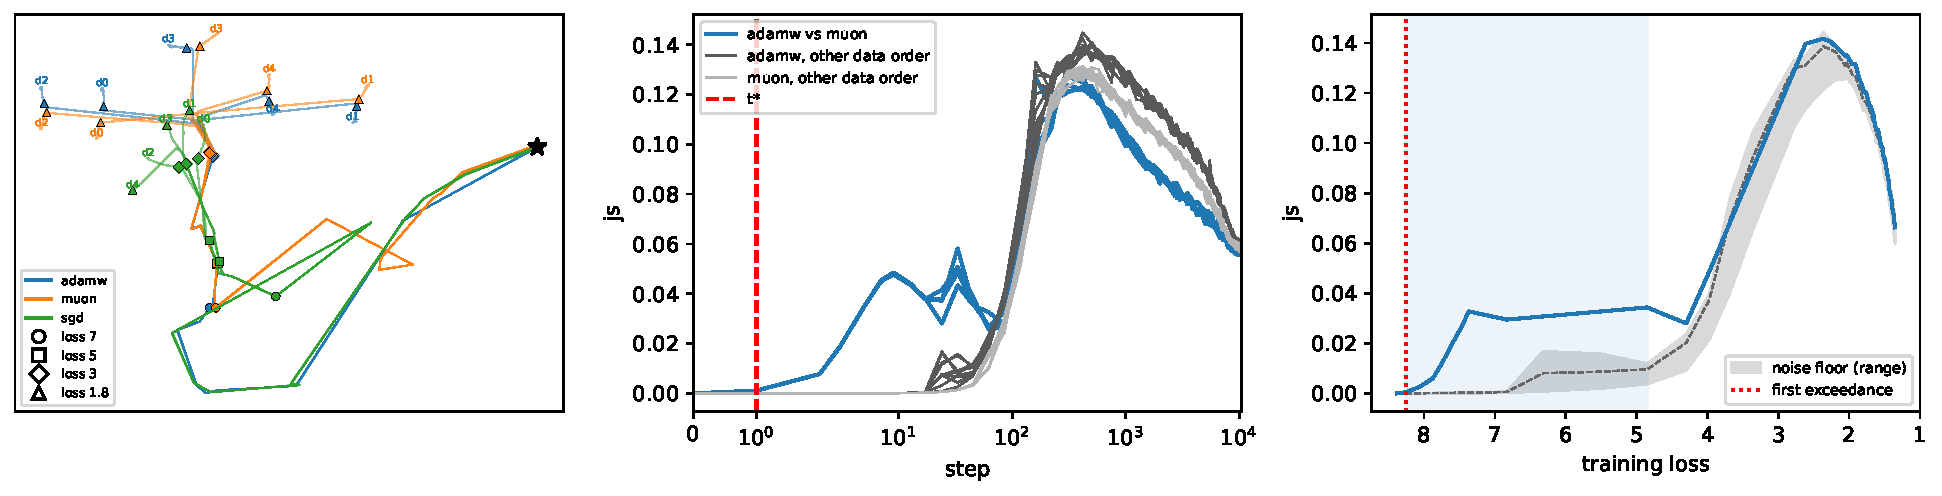
\includegraphics[width=\linewidth]{figures/ts10m/divergence_umap.pdf}
\caption{TinyStories-10M. Left: the AdamW and Muon runs on three data orders (d0--d2, at step 500) from step 250
on: densMAP of the Jensen--Shannon distance ($\sqrt{\JS}$) between all pairs of logged steps, each run
thinned to points at least 0.28 apart so its late steps do not crowd out the other runs. Black circles: step 250; markers:
fixed steps, with each run's training loss written at steps 250, 1000 and 2000. densMAP keeps neighbourhoods but
not distances. Middle: divergence between AdamW and Muon at equal steps (blue) and the data-order floor (grey);
dotted: step 250, where the left panel starts. Right: validation loss of AdamW, Muon and SGD, mean over five data
orders, band from min to max. Hyperparameters in \cref{tab:setup,tab:optim}.}
\label{fig:div}
\end{figure}

\paragraph{Approach.} We train nanoGPT models \citep{karpathy2022nanogpt} on character-level Shakespeare
(10.8M parameters) and on TinyStories (14M and 30M parameters), with SGD with momentum, AdamW, and Muon
\citep{jordan2024muon}, each at a learning rate chosen by a sweep, from a shared initialization, with five
data orders per optimizer. The distance between two runs is the Jensen--Shannon divergence and the top-1
disagreement of their next-token predictions on fixed held-out contexts. We compare runs at equal steps and
at equal training loss, and calibrate against a noise floor: the distance between two runs of the same
optimizer with different data orders. A SimpleCNN on CIFAR-10 replicates the break-even analysis of
\citet{jastrzebski2020breakeven} as a check of the pipeline.

\paragraph{Contributions.}
\begin{enumerate}[leftmargin=1.5em]
\item \textbf{Divergence curves} between every pair of optimizers in three settings, at equal steps and at
  equal training loss, against a data-order noise floor (\cref{sec:res-split}). After warmup, at equal loss,
  two optimizers are about as far apart as two data orders of one optimizer: within 1.1 times on TinyStories-30M,
  up to 1.5 times for SGD against AdamW or Muon at losses 4--2.5 on TinyStories-10M, and further only for the pairs
  with SGD on Shakespeare, where SGD barely trains. The larger ratios within warmup are inflated by a floor
  near zero.
\item \textbf{A test for a split point}: episodes\extra\ in which the distance exceeds the floor and a
  persistent split\extra, located as a loss level with a bootstrap over data orders (\cref{sec:method-split,sec:res-split}).
  There is a persistent split in 1 of 9 pairs (Muon--SGD on Shakespeare, from loss 2.82, in 96.5\% of
  resamples, lost with another metric or a stricter threshold), none between AdamW and Muon.
\item \textbf{AdamW against Muon, and optimizer against data order}\extra\ at equal steps (\cref{fig:div},
  \cref{sec:res-route}): Muon is faster, and AdamW and Muon on the same data order are at most about a fifth
  closer than two data orders of one optimizer, because they share their recent batches; at the end of
  TinyStories-30M the AdamW--Muon distance equals the data-order floor. The n-gram references show in which
  order the optimizers pass the unigram and bigram solutions.
\item \textbf{What coincides with the changes in distance}: sharpness against its optimizer-specific
  stability threshold, batch sharpness, the end of warmup (\cref{sec:res-coincide}). The edge of stability does
  not explain them: on TinyStories AdamW is at its threshold for long stretches whether or not the optimizers differ, and SGD only
  early in training. With the cosine schedule the sharpness levels off and does not follow the threshold up as the
  learning rate decays, and across learning rates\extra\ the top Hessian eigenvalue of all three optimizers falls about
  as $1/\eta$. Muon with its auxiliary AdamW matched to AdamW\extra\ still memorizes on Shakespeare, so the
  memorization comes from its updates of the hidden matrices.
\item \textbf{A causal test by swapping} optimizers at nine fork times with warm optimizer states, scored by
  where the fork lands between the two pure runs, and a basin-level test by linear mode connectivity
  (\cref{sec:res-swap}). On TinyStories-10M the optimizer that trains last decides the function whenever it is
  fast enough to: forks from SGD to AdamW or Muon land on the new optimizer even after 4000 steps, while forks
  into SGD end closer to their parent than to pure SGD from step 1500 on (step 5000 on TinyStories-30M, where
  SGD's rate is higher). In weight space the optimizer leaves a mark that function space
  does not show: forks that change the optimizer stay linearly connected to their parent only from a later fork
  step than forks that change the data order (except for Muon on Shakespeare), and between pure runs\extra\ the
  barrier between AdamW and Muon extends beyond the first block, where that between two data orders lies.
\item \textbf{The anatomy of the sharp direction}: which parameter blocks carry the top Hessian eigenvector
  and its curvature, by optimizer and over training (\cref{sec:res-anatomy}). It differs by optimizer
  (embeddings for Muon on Shakespeare, value--output matrices for Muon on TinyStories, head or gains for
  AdamW on TinyStories). At the edge of stability the sharp direction lies at the input end of the network: on
  TinyStories-10M, SGD's in blocks 1--2 (66\%), that of the operator that sets AdamW's threshold in the
  embeddings (68\%), and Muon's, of $H$, which is not its threshold operator, in blocks 1--3 (84\%). Except in
  AdamW's embeddings, most of the eigenvalue comes from curvature between layers (66\% for SGD, 71\% for Muon).
\item \textbf{A replication of the break-even point} on CIFAR-10 and its transfer to the language models
  (\cref{sec:res-breakeven}). The sharpness and gradient-noise effects replicate, but at equal training loss,
  away from the initial loss, two learning rates differ by at most about twice the floor.
\item \textbf{Controls}\extra\ (\cref{sec:res-controls}): a second initialization moves the function as much as a
  new data order and reproduces the episodes; SGD's loss gap on rare tokens is a matter of speed; learning rates
  from a quarter to four times each optimizer's rate stay within 0.8--1.1 times the floor at equal loss; and on a
  linear model, where theory predicts different limits, the same detector finds a persistent split near
  interpolation, while AdamW and Muon trained into memorization on Shakespeare still do not split.
\item \textbf{A model of the results}\extra\ (\cref{sec:theory}): at equal loss, predictors of one n-gram class
  lie within a distance of the class optimum set by the excess loss, whatever the optimizer. The bound says
  nothing far above the class optimum, as in warmup, where the update geometries pick different routes, or where
  the class has no best predictor; near it, the distance between optimizers is mostly data-order noise. Weight
  symmetries let each optimizer end at its own point of the set of weights computing one function, which
  explains the barriers. Each optimizer has a stability threshold (for Muon on a spectral-norm sharpness,
  \citealp{islamov2026noneuclidean}), and a stability cap on curvature does not choose between functions of
  equal loss. A toy bigram model reproduces these effects exactly.
\end{enumerate}
\paragraph{Planned and added analyses.} The project plan comprised the learning-rate sweeps, the divergence
curves at equal steps and at equal loss against the data-order floor, the first exceedance $t^\ast$ with a
bootstrap over data orders, its comparison with the sharpness thresholds and the end of warmup, the swaps with
warm optimizer states scored by distance and function metrics, linear mode connectivity against the fork time,
the anatomy of the top eigenvector, and the CIFAR-10 break-even check. Everything else was added after the
first results, mostly to test explanations of them, and is marked with \dag\ in the headings and captions: the episodes and
the persistent split (as $t^\ast$ turned out to be degenerate), the decomposition into optimizer and data order
and the n-gram references, the edge of stability of Muon's auxiliary AdamW and the matched control, the
robustness checks, the anatomy of AdamW's preconditioned operator, the floor-normalized swap scores and the barriers to pure runs, the scale-free weight metrics
($\|\theta\|_\infty/\|\theta\|_2$ and the stable rank) and their shifts under swaps, the representation
similarity, the layer-wise barriers, the comparison off the data distribution, the break-even runs on the
language models and with two batch sizes, the learning-rate sweeps with sharpness measurements and the
curvature between layers, the controls of \cref{sec:res-controls} (a second initialization, token frequency, a
linear positive control, Shakespeare runs trained into memorization, and other learning rates), and the model of
the results in \cref{sec:theory} with its toy model.

Code: \url{https://github.com/qqgjyx/MIT-6.7910} (\texttt{code/}).

%% =================================================================
\section{Related work}
\label{sec:related}
%% =================================================================

\paragraph{Implicit bias of optimizers.} For linear models the limit of training depends on the geometry
of the optimizer: steepest descent in a norm converges to the max-margin solution in that norm
\citep{gunasekar2018geometry}, giving $\ell_2$ for gradient descent \citep{soudry2018separable},
$\ell_\infty$ for Adam \citep{zhang2024adam}, an $\ell_\infty$-constrained KKT point for AdamW with weight
decay \citep{xie2024adamw}, and the spectral norm for Muon \citep{fan2025spectral}. Away from the limit,
finite step sizes act as implicit regularizers: for SGD the modified loss penalizes the gradient norm
\citep{smith2021origin}, while for Adam the corresponding term can have the opposite sign
\citep{cattaneo2024adam}. Empirical comparisons in deep networks are made at the end of training
\citep{wilson2017marginal,vasudeva2025rich,zhao2025deconstructing,cortesi2026same}. We look at the whole
trajectory instead.

\paragraph{Edge of stability.} With full-batch gradient descent, the top Hessian eigenvalue rises until it
reaches $2/\eta$ and then stays near it while the loss keeps decreasing \citep{cohen2021eos}; this is
explained by self-stabilization \citep{damian2023selfstab} and described by central flows
\citep{cohen2025central}. Adaptive methods reach an analogous \emph{adaptive edge of stability}, where the
top eigenvalue of the preconditioned Hessian sits at $(2+2\beta_1)/((1-\beta_1)\eta)$
\citep{cohen2022adaptive}. For mini-batch SGD, \citet{andreyev2024eoss} show that the quantity that
stabilizes at $2/\eta$ is the \emph{batch sharpness}, the curvature of mini-batch losses along their own
gradients, while $\lmax$ stays below; \citet{andreyev2026momentum} study the same regime with momentum.
\citet{islamov2026noneuclidean} extend the edge of stability to non-Euclidean gradient descent, such as the
spectral gradient descent behind Muon, where a sharpness measured in the spectral norm sits at
$2\|\nabla L\|_*/\eta$.
\citet{kalra2024warmup} relate learning-rate warmup to these sharpness dynamics. Transformer Hessians differ
strongly across parameter blocks \citep{zhang2024hessian}, which motivates our block decomposition.

\paragraph{Break-even point and early training.} \citet{jastrzebski2020breakeven} argue that early in
training SGD reaches a break-even point, after which the learning rate and batch size set the curvature and
the gradient noise along the rest of the trajectory, and show that SGD runs with different learning rates
separate early in prediction space. \citet{frankle2020lmc} find that training becomes stable to SGD noise
early: two copies trained on from the same checkpoint with different data orders end in one linearly
connected region once the checkpoint is past an early point. We use both as templates, comparing optimizers
instead of learning rates or data orders.

\paragraph{Muon and optimizer switching.} Muon \citep{jordan2024muon} updates each hidden weight matrix with
its momentum after approximate orthogonalization by a Newton--Schulz iteration, and has been scaled to
large language models \citep{liu2025muon}. SWATS \citep{keskar2017swats} switches from Adam to SGD during
training, scored by accuracy; our swaps are scored by where the function ends.

%% =================================================================
\section{Setup}
\label{sec:setup}
%% =================================================================

\paragraph{Models and data.} \Cref{tab:setup} lists the four settings. The language models are nanoGPT
\citep{karpathy2022nanogpt} with pre-LayerNorm blocks, GELU MLPs of width $4d$, no biases, no dropout, an
untied output head, and separate query, key and value projections (so that Muon orthogonalizes each and the
block decomposition of \cref{sec:method-anatomy} can separate the query-key from the value-output
matrices). The context is 256 tokens. Character-level Shakespeare uses nanoGPT's 90/10 split and a
65-character vocabulary. TinyStories \citep{eldan2023tinystories} (GPT-4 version) uses a
4096-token byte-level BPE trained on the training split, so that the head and the stored predictions stay
small. The vision check is the SimpleCNN of \citet{jastrzebski2020breakeven} (two 32-filter and two
64-filter $3\times3$ convolutions with max pooling after each pair, then a 128-unit dense layer, ReLU) on
CIFAR-10 \citep{krizhevsky2009cifar} without augmentation.

\begin{table}[t]
\centering\small
\caption{Settings. $L$ layers, model width $d$, vocabulary $V$. Parameters in parentheses exclude the token
and position embeddings and the head. LM batches are sequences $\times$ tokens. ``aux.'': learning rate of
Muon's auxiliary AdamW. CIFAR-10 settings in \cref{sec:method-breakeven}. LM schedules: linear warmup for $w$ steps, then cosine decay to
10\% of the peak learning rate at the last step. The CIFAR-10 runs use a constant learning rate.}
\label{tab:setup}
\setlength{\tabcolsep}{4.5pt}
\begin{tabular}{@{}llrrrrlll@{}}
\toprule
Setting & Model ($L$, heads, $d$, $V$) & Params & Steps & Batch & $w$ & $\eta_{\rm SGD}$ & $\eta_{\rm AdamW}$ & $\eta_{\rm Muon}$ (aux.) \\
\midrule
Shakespeare-char & 6, 6, 384, 65 & 10.8M (10.6M) & 1{,}500 & $64\times256$ & 100 & 0.05 & $3\cdot10^{-4}$ & 0.04 ($10^{-3}$) \\
TinyStories-10M & 6, 6, 384, 4096 & 13.9M (10.6M) & 10{,}000 & $128\times256$ & 200 & 0.03 & $2\cdot10^{-3}$ & 0.01 ($2\cdot10^{-3}$) \\
TinyStories-30M & 8, 8, 512, 4096 & 29.5M (25.2M) & 20{,}000 & $128\times256$ & 400 & 0.1 & $2\cdot10^{-3}$ & 0.01 ($1.5\cdot10^{-3}$) \\
CIFAR-10 & SimpleCNN, ReLU & 0.36M & 39{,}000 & 128 & -- & \multicolumn{3}{l}{plain SGD, $\eta\in\{0.001,0.01,0.1\}$} \\
\bottomrule
\end{tabular}
\end{table}

Shakespeare runs take 24.6M tokens (about 24 passes over the 1M training characters). Without dropout the
validation loss is lowest near step 1000 and rises after, so these runs stop at 1500 steps. The TinyStories
runs take 328M and 655M tokens (about 0.6 and 1.2 epochs).

\paragraph{Optimizers.} Write $g_t$ for the mini-batch gradient at step $t$ and $\eta_t=\eta\,\varphi(t)$
for the learning rate, with $\varphi(t)=(t+1)/w$ for $t<w$ and
$\varphi(t)=0.1+0.45\,(1+\cos(\pi\,(t-w)/(T-w)))$ after, $T$ being the last step.
\begin{itemize}
\item \textbf{SGD} with heavy-ball momentum $\mu=0.9$ and no weight decay:
  $b_{t+1}=\mu b_t+g_t$, $\theta_{t+1}=\theta_t-\eta_t b_{t+1}$.
\item \textbf{AdamW} with $(\beta_1,\beta_2)=(0.9,0.95)$ ($(0.9,0.99)$ for Shakespeare, as in nanoGPT),
  $\epsilon=10^{-8}$, and decoupled weight decay $0.1$ on every tensor with at least two dimensions
  (including embeddings and head) and none on LayerNorm gains:
  $\theta_{t+1}=(1-\eta_t\lambda_{\rm wd})\theta_t-\eta_t\,\hat m_{t+1}/(\sqrt{\hat v_{t+1}}+\epsilon)$, with
  bias-corrected moments $\hat m,\hat v$.
\item \textbf{Muon} \citep{jordan2024muon} on every matrix inside the transformer blocks (query, key, value,
  attention output, both MLP matrices), with momentum $\beta=0.95$, Nesterov, and no weight decay:
  $M_{t+1}=\beta M_t+(1-\beta)G_t$, $W_{t+1}=W_t-\eta_t\sqrt{\max(1,n_{\rm out}/n_{\rm in})}\,
  \mathrm{NS}_5\big((1-\beta)G_t+\beta M_{t+1}\big)$, where $\mathrm{NS}_5$ is five steps of the quintic
  Newton--Schulz iteration that approximates the orthogonal polar factor. Embeddings, head and gains are
  updated by an auxiliary AdamW with $(0.9,0.95)$, $\epsilon=10^{-8}$, no weight decay, and its own learning
  rate (\cref{tab:setup}). This matches the reference implementation \citep{jordan2024muon} in the
  Newton--Schulz settings, the Nesterov momentum of 0.95, the shape scaling and the split of parameters between
  Muon and AdamW.
\end{itemize}
Gradient clipping is off, since it would hide edge-of-stability dynamics. Training steps of the language
models use bfloat16 autocast; all measurements (\cref{sec:methods}) are in float32, with TF32 matrix products on the GPU.

\paragraph{Learning rates.} For each setting and optimizer we ran five learning rates (grids in
\cref{tab:sweep}) on data order 0, with the schedule and length of the main runs and no measurements, and
kept the one with the best final validation loss (on the validation sequences of the probe, \cref{sec:method-distance}). Shakespeare is the exception: since its runs overfit, we
kept the best \emph{minimum} validation loss over training. SGD is the exception to the rule: in every
setting its best rate on data order 0 diverged or blew up on other data orders (0.2 on Shakespeare, 0.1 on
TinyStories-10M, 0.3 on TinyStories-30M), so SGD uses a lower rate: 0.05 on Shakespeare (the smallest of its
grid) and the next lower rate on TinyStories, 0.03 and 0.1. On Shakespeare every SGD rate of the grid stops
at about the same minimum validation loss (2.44--2.50, the bigram level), so we took the smallest and most
stable one. Runs whose training loss became non-finite were stopped and counted as diverged. Only the
learning rates were tuned, in the same way for every optimizer; all other hyperparameters are fixed
(\cref{tab:optim}).

\paragraph{Shared initialization and data order.} Every run starts from the same initialization (seed 0).
The mini-batch at step $t$ depends only on the data order $d$ and on $t$: for the language models it is
$B$ windows of 256 tokens at offsets drawn uniformly from the training split by a generator seeded with
$(d,t)$; for CIFAR-10 it is a slice of a per-epoch permutation seeded with $(d,\text{epoch})$, dropping the
last incomplete batch. Two runs with the same $d$ therefore see identical batches whatever their optimizer,
and forks and resumed runs see the batches their parent would have seen. Batches used for measurements come
from separate random streams and never change the training order. Each optimizer is run with data orders
$d\in\{0,\dots,4\}$: 15 main runs per setting. The runs with $d=0$ also keep the other optimizers' states
in shadow and save fork checkpoints (\cref{sec:method-swap}).

\paragraph{Control for Muon's auxiliary Adam.\extra} On Shakespeare, Muon's auxiliary AdamW and the AdamW runs differ
in learning rate ($10^{-3}$ against $3\cdot10^{-4}$), $\beta_2$ (0.95 against 0.99) and weight decay (none
against 0.1). A control suite repeats Muon with its auxiliary AdamW matched to AdamW (learning rate
$3\cdot10^{-4}$, $\beta=(0.9,0.99)$, weight decay 0.1, which here also applies to the gains), with data
orders 0--4 (``matched Muon''). It differs from AdamW only in how the hidden matrices are trained (and in
decay on the gains).

%% =================================================================
\section{Methods}
\label{sec:methods}
%% =================================================================
Step $s$ always refers to the model $\theta_s$ after $s$ updates ($s=0$ is the initialization). Each run
logs predictions at its prediction steps $\cS$ and curvature at its measurement steps $\cM$; both grids
combine a linear and a log-spaced grid (\cref{tab:grids}).

\subsection{Function distance and alignment}
\label{sec:method-distance}

\paragraph{Distance.} Every run stores, at each $s\in\cS$, its next-token distributions on a fixed set of
$N$ held-out positions, identical across runs: for Shakespeare all 256 positions of 64 validation sequences
($N=16{,}384$), for TinyStories 16 evenly spaced positions of 128 validation sequences ($N=2{,}048$), and
for CIFAR-10 the 10{,}000 test images. Write $p_i^X(s)$ for the distribution of run $X$ at step $s$ on
position $i$. The distance between run $X$ at step $s$ and run $Y$ at step $s'$ is the mean Jensen--Shannon
divergence in bits,
\begin{equation}
D_{\JS}(X_s,Y_{s'})=\frac1N\sum_{i=1}^N\JS\big(p_i^X(s),\,p_i^Y(s')\big),\qquad
\JS(p,q)=\tfrac12\KL(p\,\|\,m)+\tfrac12\KL(q\,\|\,m),\quad m=\tfrac12(p+q),
\label{eq:js}
\end{equation}
with base-2 logarithms, so $D_\JS\in[0,1]$. The second distance is the top-1 disagreement
$D_{\rm dis}(X_s,Y_{s'})=1-\frac1N\sum_i\mathbf 1\{\argmax_v p^X_{i,v}(s)=\argmax_v p^Y_{i,v}(s')\}$.

\paragraph{Alignment by step.} $D(X_s,Y_s)$ at the steps $s\in\cS$ that both runs log.

\paragraph{Pictures of trajectories.\extra} To draw several runs at once we embed their logged steps in two
dimensions with densMAP, a variant of UMAP that also keeps local density, applied to the Jensen--Shannon
distance $\sqrt{\JS}$ (a metric) between all pairs of steps. densMAP and UMAP keep neighbourhoods, not
distances, so distances are read from the curves at equal steps or equal loss, never from the embedding. Late
in training the logged steps of a run lie close together and would crowd out the other runs, so each run is
thinned to points at least a fixed distance apart (0.28 in $\sqrt{\JS}$ in \cref{fig:div}).

\paragraph{Alignment by training loss.} Optimizers progress at different speeds, and comparing at equal steps
confounds ``faster'' with ``different''. Each run therefore also logs, at each $s\in\cS$, its mean
cross-entropy $\ell_X(s)$ on a fixed training probe, the same for all runs (64 training sequences, all
positions, for the language models; 2{,}000 training images for CIFAR-10). We make it monotone with a
running minimum, $\bar\ell_X(s)=\min\{\ell_X(s'):s'\in\cS,\ s'\le s\}$. Each step $s$ of $X$ is matched with
the earliest step of $Y$ whose loss is closest,
\begin{equation}
\pi_{XY}(s)=\min\Big(\argmin_{s'\in\cS}\,\big|\bar\ell_Y(s')-\bar\ell_X(s)\big|\Big),\qquad
\text{kept if }\big|\bar\ell_Y(\pi_{XY}(s))-\bar\ell_X(s)\big|\le\tau\,\bar\ell_X(s),
\label{eq:match}
\end{equation}
with $\tau=0.02$. The kept matches give points $\big(\bar\ell_X(s),\,D(X_s,Y_{\pi_{XY}(s)})\big)$, and the
\emph{loss-matched distance} $\Dloss_{X,Y}(\ell)$ is their piecewise-linear interpolation in $\ell$ (where
several steps share a loss value, the earliest is used), undefined outside the range of kept losses. The
loss coordinate is that of the first run, $X$.

\paragraph{Noise floor.} Two runs of the same optimizer from the same initialization with different data
orders, $\Dloss_{O_d,O_{d'}}$ with $d\neq d'$, differ only through the sampling of mini-batches. A difference
between optimizers counts only where it exceeds this floor.

\subsection{Locating the split}
\label{sec:method-split}

Fix two optimizers $A$ and $B$ and write $A_d,B_d$ for their runs with data order $d\in\cD=\{0,\dots,4\}$.
Runs with the same $d$ share initialization and batches, so they form the \emph{cross} pairs; runs of one
optimizer with different $d$ form the \emph{floor} pairs:
\[
c_d(\ell)=\Dloss_{A_d,B_d}(\ell),\qquad f^O_{dd'}(\ell)=\Dloss_{O_d,O_{d'}}(\ell)\quad(O\in\{A,B\},\ d<d').
\]

\paragraph{Loss grid.} Let $\ell_1>\ell_2>\dots>\ell_J$ be the distinct values of $\bar\ell_{A_0}(s)$,
$s\in\cS$, that lie in the range covered by all $2|\cD|$ runs,
\[
\Big[\max_X\min_{s\in\cS}\bar\ell_X(s),\ \min_X\max_{s\in\cS}\bar\ell_X(s)\Big].
\]
Decreasing loss is the order of training.

\paragraph{Statistic.} For a multiset $S$ of data orders with distinct elements $U(S)$, let
\begin{equation}
\bar c_S(\ell)=\mean_{d\in S}\,c_d(\ell),\qquad
F_S(\ell)=\max\Big(\mean_{d<d'\in U(S)}f^A_{dd'}(\ell),\ \mean_{d<d'\in U(S)}f^B_{dd'}(\ell)\Big),
\label{eq:floor}
\end{equation}
where the cross mean counts repeated orders with their multiplicity, means skip undefined values, and the
maximum takes the defined side if only one is. The floor is thus the larger of the two optimizers'
average seed-to-seed distances. A level is \emph{above the floor} if the cross distance exceeds the floor by
a margin,
\begin{equation}
o_S(j)=\mathbf 1\big\{\bar c_S(\ell_j)>(1+m_\times)\,F_S(\ell_j)+m_+\big\},
\label{eq:over}
\end{equation}
with $m_\times=0.5$ and $m_+=0$; a comparison with an undefined value counts as false.

\paragraph{First exceedance.} The first grid level from which the cross distance is above the floor at $k=3$
consecutive levels,
\begin{equation}
t^\ast(S)=\ell_{j^\ast},\qquad
j^\ast=\min\big\{j:\ o_S(i)=1\ \text{ for } i=j,\dots,j+k-1\big\},
\label{eq:tstar}
\end{equation}
undefined if no such $j$ exists. Since the grid is made of the losses of $A_0$ at its prediction steps, the
$k$ levels are consecutive distinct loss values of that run. This was the planned definition of the split, but
it is degenerate: at initialization all runs compute the same function, so the floor is close to 0 for the
first steps, while two different optimizers move apart from their first update. In every pair of optimizers
$t^\ast$ is one of the first grid levels, reached at steps 1--8 (\cref{tab:tstar}). It records that two
optimizers differ from the start, not that they split. We therefore also report:

\paragraph{Episodes and persistent split.\extra} An \emph{episode} is a maximal run of consecutive levels
$\ell_{j_0},\dots,\ell_{j_1}$ with $o_S(j)=1$ that contains at least $k$ levels ($j_1-j_0+1\ge k$), reported
as the loss range $[\ell_{j_0},\ell_{j_1}]$. The \emph{persistent split} $t^\ast_{\rm p}(S)$ is the start
$\ell_{j_0}$ of the last episode if that episode ends at the last level of the grid ($j_1=J$), and undefined
otherwise: the loss from which the cross distance stays above the floor down to the lowest loss that all runs
reach. A persistent split is what ``together first, apart later'' predicts; an episode that ends before $\ell_J$
is a difference that later disappears. Figures also show the ratio $\bar c_\cD(\ell)/F_\cD(\ell)$ against the
loss, with the threshold $1+m_\times$.

\paragraph{Estimate and uncertainty.} The point estimates are $t^\ast=t^\ast(\cD)$, $t^\ast_{\rm p}=
t^\ast_{\rm p}(\cD)$ and the episodes of $\cD$. For their uncertainty we draw 1000 bootstrap resamples $S_b$ of
$|\cD|$ data orders with replacement and report, for $t^\ast$ and $t^\ast_{\rm p}$ separately, the 2.5 and
97.5 percentiles of the defined values, together with the fraction of resamples in which one is found (a
resample with a single distinct order has no floor and gives none). The distance is $D_\JS$; $D_{\rm dis}$
and other values of $m_\times$, $k$ and $\tau$ are checked in \cref{sec:res-split} (300 resamples each).

\paragraph{In steps.} $t^\ast$ is a loss level, which makes it comparable across optimizers that reach it at
different steps. For each run $X$, $t^\ast_X=\min\{s\in\cS:\bar\ell_X(s)\le t^\ast\}$ is the first step at
which $X$ reaches it, and likewise $t^\ast_{{\rm p},X}$ for the persistent split.

\subsection{Optimizer against data order, and n-gram references\extra}
\label{sec:method-route}

\paragraph{Decomposition at equal steps.} For two optimizers $X,Y$ with data orders $d=0,\dots,n-1$ ($n=5$)
and $d^+=(d+1)\bmod n$, we compare at each shared prediction step $s$ four families of $n$ pairs:
$D(X^d_s,Y^d_s)$ (other optimizer, same data: the cross pairs above), $D(X^d_s,Y^{d^+}_s)$ (other
optimizer, other data), and the floors $D(X^d_s,X^{d^+}_s)$ and $D(Y^d_s,Y^{d^+}_s)$ (same optimizer, other
data), and plot the median and range over $d$. If the same-data distance is no larger than the floors, the
change of optimizer changes the function no more than a change of data order; if it is smaller than the
other-data distance, sharing the batches keeps the two optimizers closer.

\paragraph{N-gram references.} From the counts $n(b)$ and $n(a,b)$ of tokens and of consecutive token pairs
in the training split we build a unigram model $p_1(b)\propto n(b)+1$ and a bigram model smoothed towards it,
$p_2(b\mid a)=\big(n(a,b)+\alpha\,p_1(b)\big)/\big(n(a)+\alpha\big)$ with $\alpha=1$, evaluated at the
validation probe positions (the bigram conditioned on the current token). For a run $X$ we plot
$D_\JS$ \eqref{eq:js} between $p^X(s)$ and each reference against the training loss $\bar\ell_X(s)$. A
minimum near zero means the run passes through that n-gram solution; two optimizers that pass through it at
the same loss meet there in function space.

\subsection{Sharpness and stability thresholds}
\label{sec:method-sharpness}

At each $s\in\cM$, before the update of that step, we measure on $\theta_s$ (in float32, with TF32 matrix products):

\paragraph{Sharpness.} $\lmax$ is the largest eigenvalue of the Hessian $H=\nabla^2L_{\mathcal H}(\theta_s)$ of
the mean cross-entropy on a fixed batch $\mathcal H$ of training examples (32 sequences of 256 tokens for
the language models; 2{,}500 images, 5\% of the training set, for CIFAR-10), computed by Lanczos with full
reorthogonalization (20 iterations from a fixed random start) on Hessian-vector products. The curvature is
thus that of the training loss on fixed training sequences, while the predictions compared in
\cref{sec:method-distance} are on held-out validation contexts.

\paragraph{SGD threshold.} On a quadratic with curvature $\lambda$, heavy-ball momentum as above is stable if
and only if $\eta\lambda<2+2\mu$. We compare $\lmax(\theta_s)$ with $(2+2\mu)/\eta_s$, which is $3.8/\eta_s$
for $\mu=0.9$ and $2/\eta$ for the plain SGD of the break-even runs.

\paragraph{AdamW preconditioned sharpness.}
\label{sec:method-precond}
Following \citet{cohen2022adaptive}, let
$P=(1-\beta_1^t)\diag(\sqrt{\hat v}+\epsilon)$, with $\hat v=v/(1-\beta_2^t)$ built from the optimizer's
current second-moment state and step count $t$. The AdamW update is then $-\eta_tP^{-1}m$ with $m$ the
uncorrected first moment, so with $P$ frozen and weight decay ignored it is heavy-ball momentum with
coefficient $\beta_1$ and step $\eta_t(1-\beta_1)$ in the metric $P$. It is stable if
$\lmax(P^{-1}H)<(2+2\beta_1)/((1-\beta_1)\eta_t)$, which is $38/\eta_t$ for $\beta_1=0.9$. We compute the
preconditioned sharpness $\lmax(P^{-1/2}HP^{-1/2})$, which has the spectrum of $P^{-1}H$, by the same
Lanczos procedure, for every run that trains with AdamW (including forks into AdamW).

\paragraph{Batch sharpness.} Following \citet[Def.~1]{andreyev2024eoss},
\begin{equation}
\mathrm{BS}(\theta)=\frac{\sum_{j=1}^n g_j^\top H_j\,g_j}{\sum_{j=1}^n\|g_j\|^2},
\label{eq:bs}
\end{equation}
where $g_j$ and $H_j$ are the gradient and Hessian of the loss on mini-batch $j$, over $n=8$ random
training mini-batches of the training batch size (a fresh random stream at every measured step). For
mini-batch SGD without momentum, \citet{andreyev2024eoss} find that $\mathrm{BS}$ stabilizes at $2/\eta$. We
measure it for every optimizer and compare it with $(2+2\mu)/\eta_s$ for SGD.

\paragraph{Muon.} Muon's update on a hidden matrix is orthogonalized, with all singular values near one
whatever the size of the gradient, so the quadratic argument above, where the step scales with the gradient,
does not carry over, and $\lmax(H)$ is not the quantity its threshold applies to.
\citet{islamov2026noneuclidean} show that for such scale-invariant updates the stability condition bounds a
sharpness measured in the spectral norm by $2\|\nabla L\|_*/\eta$, with $\|\cdot\|_*$ the nuclear norm, and that
full-batch spectral gradient descent sits at this bound (\cref{sec:theory}). We have not yet measured this
spectral-norm sharpness (\cref{sec:discussion}); here we report Muon's $\lmax$ and batch sharpness without a
threshold. What we can test against a threshold is the part of the model that Muon leaves to its auxiliary
AdamW (\cref{sec:method-aux}).

\paragraph{One-step loss change.} $\Delta L(s)=\ell_X(s)-\ell_X(s+1)$ on the training probe, used in the
break-even analysis.

\paragraph{Edge of stability of the Adam-managed block.\extra}
\label{sec:method-aux}
Muon trains the embeddings, head and gains with an auxiliary AdamW; write $a$ for these coordinates. At the
fork checkpoints of the $d=0$ runs (\cref{tab:forks}), which hold the optimizer states, we compute the top
eigenvalue of $P_a^{-1/2}H_{aa}P_a^{-1/2}$, where $H_{aa}$ is the block of the Hessian on $\mathcal H$ restricted
to $a$ and $P_a$ the preconditioner $P$ defined above, built from the state of the run's own Adam for
these coordinates (Muon's auxiliary AdamW, or AdamW itself), by the same Lanczos procedure. We compare it with
$(2+2\beta_1)/((1-\beta_1)\eta_s)$, with $\eta$ and $\beta_1$ of that Adam. This treats the block as if the
rest of the model were frozen, so it is a check of the auxiliary AdamW on its own, not a threshold for Muon.

\paragraph{What coincides with the split.} For a sharpness measure $\mathcal{Q}$ with threshold
$\Theta$, the measured steps at the edge of stability are
$\mathcal E(X)=\{s\in\cM:\mathcal{Q}_X(s)\ge(1-\delta)\,\Theta_X(s)\}$ with $\delta=0.1$. We report the onset
$s_{\rm EoS}(X)=\min\mathcal E(X)$, the last step of $\mathcal E(X)$, and the fraction $|\mathcal E(X)|/|\cM|$
of measured steps at the edge of stability, for $\lmax$ (SGD) and the preconditioned sharpness (AdamW), and
the ratio $\mathcal Q_X(s)/\Theta_X(s)$ at the steps $t^\ast_X$ and $t^\ast_{{\rm p},X}$. Since $\cM$ is
partly log-spaced, the fraction weights early training more than a fraction of steps would. Batch sharpness
is shown in the figures but has no onset computed. We compare these with $t^\ast_X$ and $t^\ast_{{\rm p},X}$,
with the episodes, with the end of warmup $w$, and with the loss levels across settings.

\paragraph{Sharpness across learning rates.\extra} To see how each optimizer's sharpness scales with the learning
rate, we repeated part of the sweeps on data order 0 with the sharpness measurements of the main runs: on
TinyStories-10M SGD at 0.01, 0.03 and 0.1, AdamW at $10^{-3}$, $2\cdot10^{-3}$ and $4\cdot10^{-3}$, and Muon at
0.005, 0.01, 0.02 and 0.04; on Shakespeare the five rates of each optimizer in \cref{tab:sweep}. The plateau of a
run is the median of its sharpness over the steps after warmup with $\varphi(t)\ge0.8$, and we fit a line to
the logarithm of the plateau against that of the peak rate $\eta$. A slope of $-1$ means that the run sits at the
same fraction of a threshold proportional to $1/\eta$ at every rate.

\subsection{Swaps with warm optimizer states}
\label{sec:method-swap}

\paragraph{Shadow states.} During each $d=0$ run of optimizer $A$, the other two optimizers are stepped on the
same mini-batch gradients with learning rate 0. The state updates of SGD momentum, AdamW and Muon do not
depend on the learning rate, and with learning rate 0 neither the update nor the decoupled weight decay moves
the parameters; so their momenta, second moments and step counts evolve as if they were training, while the
parameters follow $A$ alone. (Our copy of Muon does not overwrite the gradient in place, so a shadow
optimizer stepping after it sees the same gradient.)

\paragraph{Forks.} At fork steps $s$ (nine per setting, \cref{tab:forks}), the $d=0$ run saves $\theta_s$ and
the states of all three optimizers. The fork $A\to B$ at $s$ loads $\theta_s$ and $B$'s shadow state, keeps
$B$'s own hyperparameters and learning rate, and continues from $s$ to $T$ on the same schedule $\varphi$ and
the same batches. All six ordered pairs are forked at all nine steps. The control ``$A$ continued with the
same batches'' is the parent run itself. In addition, $A$ is forked into $A$ with data order 1 at the same
steps, the control for mode connectivity (\cref{sec:method-lmc}). This gives 81 forks per language-model
setting. Forks log predictions and measurements like their parents.

\paragraph{Where a fork lands.} Let $F$ be the final model of the fork $A\to B$ at $s$, $A$ the final model of
the parent $A_0$, and $B$ the final model of the pure run $B_0$ (from initialization, same batches). With $D$
either distance of \cref{sec:method-distance}, the landing coordinate is
\begin{equation}
r=\frac{D(F,A)}{D(F,A)+D(F,B)},
\label{eq:landing}
\end{equation}
which is 0 at $A$'s function and 1 at $B$'s. It is a ratio of distances, not a projection: a fork far from
both ends has $r$ near $1/2$, so we report $D(F,A)$, $D(F,B)$ and $D(A,B)$ with it. We also give $D(F,B)$ over the final data-order floor
of $B$, and $D(F,A)$ over that of $A$\extra: a fork within one floor of a pure run is as close to it as another
data order is. For each function metric
$\phi$ of \cref{sec:method-metrics} we also report the shift $(\phi(F)-\phi(A))/(\phi(B)-\phi(A))$, the
fraction of the gap between the pure runs that the swap closes. If the function is decided at the split,
forks with $s<t^\ast_A$ should end near $r=1$ and forks with $s>t^\ast_A$ near $r=0$. Since $t^\ast$ turns out to be
degenerate (\cref{sec:method-split}), the time to compare fork steps with is the end of the early episode.

\subsection{Linear mode connectivity}
\label{sec:method-lmc}

For two final weight vectors $\theta_1,\theta_2$ of the same architecture let
$L(\alpha)$ be the mean cross-entropy of $(1-\alpha)\theta_1+\alpha\theta_2$ (every floating-point entry of
the state interpolated) on the 64 sequences of the training probe. The barrier is
\begin{equation}
\mathrm{Bar}(\theta_1,\theta_2)=\max_{\alpha\in\{0,0.1,\dots,1\}}\big[L(\alpha)-(1-\alpha)L(0)-\alpha L(1)\big],
\label{eq:barrier}
\end{equation}
a loss version of the instability of \citet{frankle2020lmc}. We compute it between the parent $A_0$ and each
of its forks, as a function of the fork step: the forks $A\to A$ with data order 1 reproduce the instability
analysis of \citet{frankle2020lmc} for each optimizer, and the forks $A\to B$ ask whether a change of
optimizer at $s$ leaves the solution in the same basin.

\subsection{Anatomy of the top eigenvector}
\label{sec:method-anatomy}

Partition the parameters into blocks: \emph{emb} (token and position embeddings); for each layer $i$,
\emph{qk}$_i$ ($W_Q,W_K$), \emph{ov}$_i$ ($W_V$ and the attention output $W_O$) and \emph{mlp}$_i$ (both MLP
matrices); \emph{norms} (all LayerNorm gains); and \emph{head}. For the CNN each layer is a block. Let $v$ be
the unit top eigenvector of $H$ returned by Lanczos, and $v_b$ the vector equal to $v$ on the coordinates of
block $b$ and zero elsewhere. Since the blocks partition the coordinates, $v=\sum_bv_b$ and
$\sum_b\|v_b\|^2=1$, and expanding the quadratic form gives
\begin{equation}
\lmax=v^\top Hv=\sum_b s_b+\chi,\qquad s_b=v_b^\top H_{bb}v_b,\qquad \chi=\sum_{b\neq c}v_b^\top H_{bc}v_c,
\label{eq:anatomy}
\end{equation}
where $H_{bc}$ is the block of $H$ with rows in $b$ and columns in $c$ (and $v_b$ is read as its restriction
to block $b$ where needed). We record, for each block, its share of the direction $\|v_b\|^2$ and its
self-curvature $s_b$, and the cross-block remainder $\chi=v^\top Hv-\sum_bs_b$, with $v^\top Hv$ from one more
Hessian-vector product (it equals the Lanczos estimate of $\lmax$ up to the Lanczos error). Both $s_b$ and
$\chi$ can be negative, and $s_b\le\lmax(H_{bb})\|v_b\|^2$: a block carries a large part of the sharpness only
if the direction lies in it and its own diagonal block is curved along it, while a large $\chi$ means the
sharp direction comes from interactions between blocks. The split of the project plan, $v_b^\top(Hv)_b$,
equals $\lmax\|v_b\|^2$ for an exact eigenvector and so repeats the direction share; this is why we use
\eqref{eq:anatomy} instead. For AdamW runs we repeat\extra\ the decomposition for $P^{-1/2}HP^{-1/2}$ and its top
eigenvector, whose diagonal blocks are $P_b^{-1/2}H_{bb}P_b^{-1/2}$. Figures sum blocks by type (all
\emph{qk}, all \emph{ov}, all \emph{mlp}) or by layer. Since $\chi$ counts every pair of distinct blocks, it
includes the curvature between the attention and MLP matrices of one layer. For the curvature between
layers\extra\ we recompute, at saved checkpoints, the whole matrix $v_\ell^\top Av_m$ over layers $\ell,m$
(embeddings, blocks $1,\dots,L$, and the head with the final LayerNorm), with $A=H$ for SGD and Muon and
$A=P^{-1/2}HP^{-1/2}$ for AdamW; its entries sum to $\lmax(A)$, and its off-diagonal part is the curvature
between layers. The same matrix over sublayers splits each block into its attention and its MLP, each with the
LayerNorm that feeds it.

\subsection{Function metrics}
\label{sec:method-metrics}

Offline, on saved checkpoints, we compute three groups of metrics at fixed validation points (definitions in
\cref{app:metrics}). \emph{Input derivatives} of the loss as a function of the input (the token embeddings
for the language models), from first to third order: gradient norm, Jacobian norm of the softmax output
\citep{novak2018sensitivity}, Frobenius norm and top eigenvalue of the input Hessian
\citep{moosavi2019cure}, level-set curvature \citep{srinivas2022lowcurv}, and three third-order
quantities. \emph{Weight norms}: those linear theory predicts each optimizer keeps small ($\ell_2$,
$\ell_\infty$, spectral), and norm-based measures compared by \citet{jiang2020fantastic}. \emph{Accuracy and
robustness}: Gaussian input noise for the CNN \citep{ford2019noise} and one-token substitution sensitivity
\citep{hahn2021sensitivity} for the language models. \emph{Representations}\extra: linear CKA
\citep{kornblith2019cka} between the final hidden states of two runs after each transformer block and after the
final LayerNorm, on 64 training sequences, for pairs of pure runs that differ only in the optimizer, only in the
data order, or in the initialization.

\subsection{Break-even replication}
\label{sec:method-breakeven}

We follow the protocol of \citet{jastrzebski2020breakeven}: plain SGD (no momentum) at a constant learning
rate, without warmup, as they do; our main language-model runs instead use warmup and cosine decay to 10\% of the
peak rate. Besides $\lmax$ (their $\lambda_H^1$) and $\Delta L$, at each measured step we draw
$L=25$ mini-batch gradients $g_1,\dots,g_L$ and estimate the gradient covariance
$\hat K=\frac1L\sum_i(g_i-\bar g)(g_i-\bar g)^\top$ through the eigendecomposition of its $L\times L$ Gram
matrix. We record its top eigenvalue $\lambda_K^1$, its smallest non-zero eigenvalue $\lambda_K^\ast$
($\hat K$ has rank at most $L-1$), $\operatorname{Tr}\hat K$, and $\|g\|/\|g_5\|$, the mean over $i$ of
$\|g_i\|/\|\Pi_5g_i\|$ with $\Pi_5$ the projection on the top five eigenvectors of $\hat K$. Prediction
trajectories are embedded in two dimensions (PCA, then UMAP; \cref{app:measure}).

\paragraph{Runs.} CIFAR-10: learning rates 0.001, 0.01 and 0.1 at batch size 128 (39{,}000 steps, 100
epochs), and batch sizes\extra\ 30 and 300 at learning rate 0.05 (also 100 epochs), with $\hat K$ always from
batch-128 gradients; two data orders each. Shakespeare and TinyStories-10M\extra: learning rates 0.03, 0.1 and 0.3
at the training batch size, with the setting's model and length; three data orders each. A rate of 1.0
diverged within 15 (Shakespeare) and 20 (TinyStories-10M) steps and was dropped. The split analysis
of \cref{sec:method-split} applied to two learning rates instead of two optimizers measures the separation of
trajectories in prediction space.

\FloatBarrier
%% =================================================================
\section{Results}
\label{sec:results}
%% =================================================================

\subsection{Learning-rate sweeps}
\label{sec:res-sweep}

\Cref{fig:sweep} (\cref{app:figures}) shows the sweeps. On both TinyStories models Muon reaches the lowest
validation loss, then AdamW, then SGD: best final validation loss 1.305, 1.339 and 1.914 on TinyStories-10M and
1.181, 1.201 and 1.340 on TinyStories-30M (SGD at its best rate on data order 0; 1.957 and 1.370 at the rates
we use), and in the main runs AdamW takes 1.35 and 1.22 times as many steps as Muon to reach its own final
validation loss. On Shakespeare AdamW reaches the lowest, then Muon, then SGD: best minimum validation loss
1.54, 1.56 and 2.44 (2.50 for SGD at 0.05, about the loss at which all three optimizers pass the bigram model, \cref{sec:res-route}). SGD at 1 and 3 diverged on
both TinyStories models. Without dropout the Shakespeare runs overfit, Muon fastest: its validation loss is
lowest near step 500 and ends at 2.84--2.88 in the main runs, against 1.54--1.55 for AdamW (\cref{fig:losses}).

\subsection{Divergence curves and the split}
\label{sec:res-split}

\begin{figure}[t]
\centering
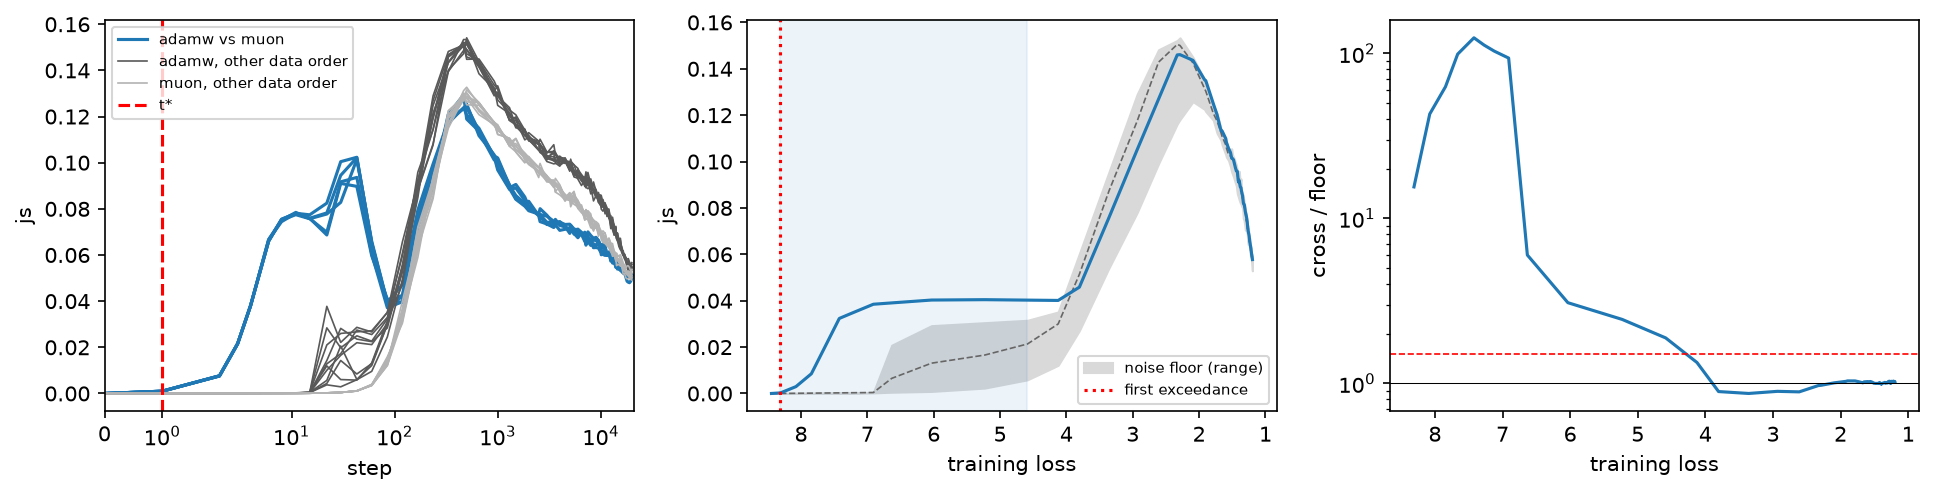
\includegraphics[width=0.9\linewidth]{figures/ts30m/divergence_adamw_muon.png}\\
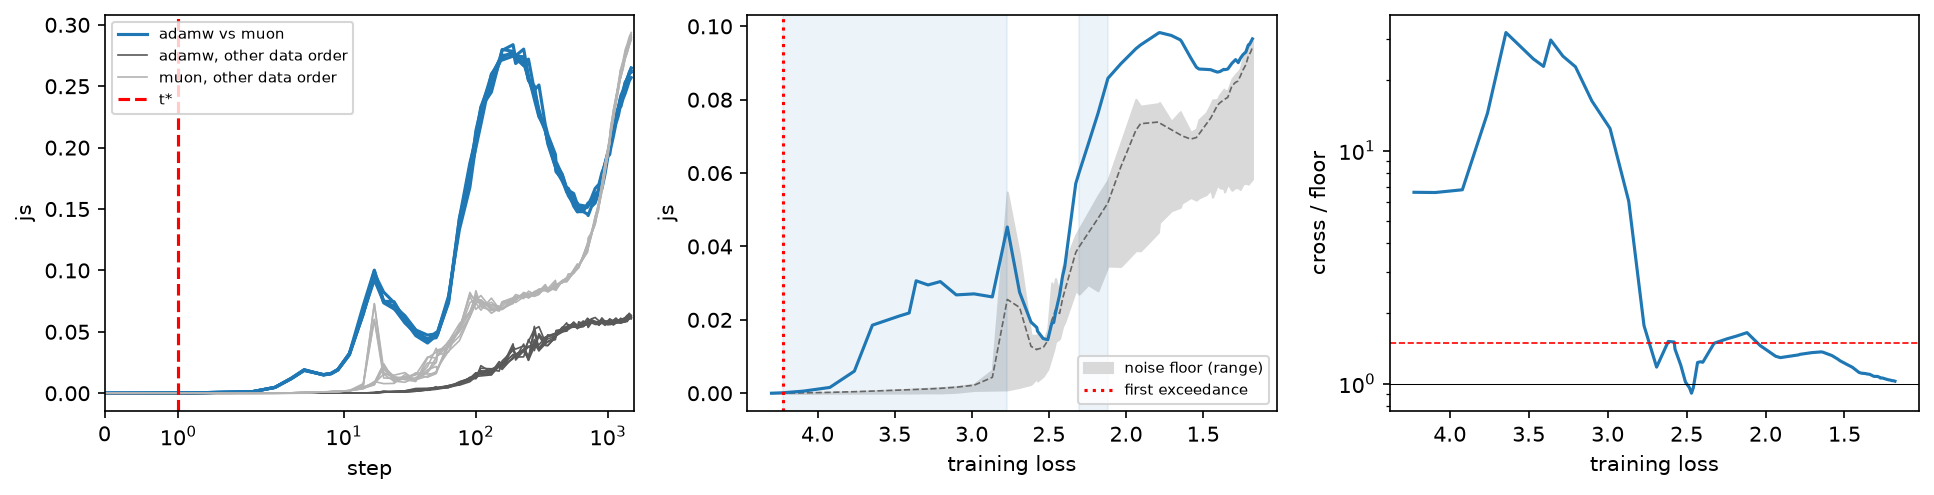
\includegraphics[width=0.9\linewidth]{figures/shakespeare/divergence_adamw_muon.png}\\
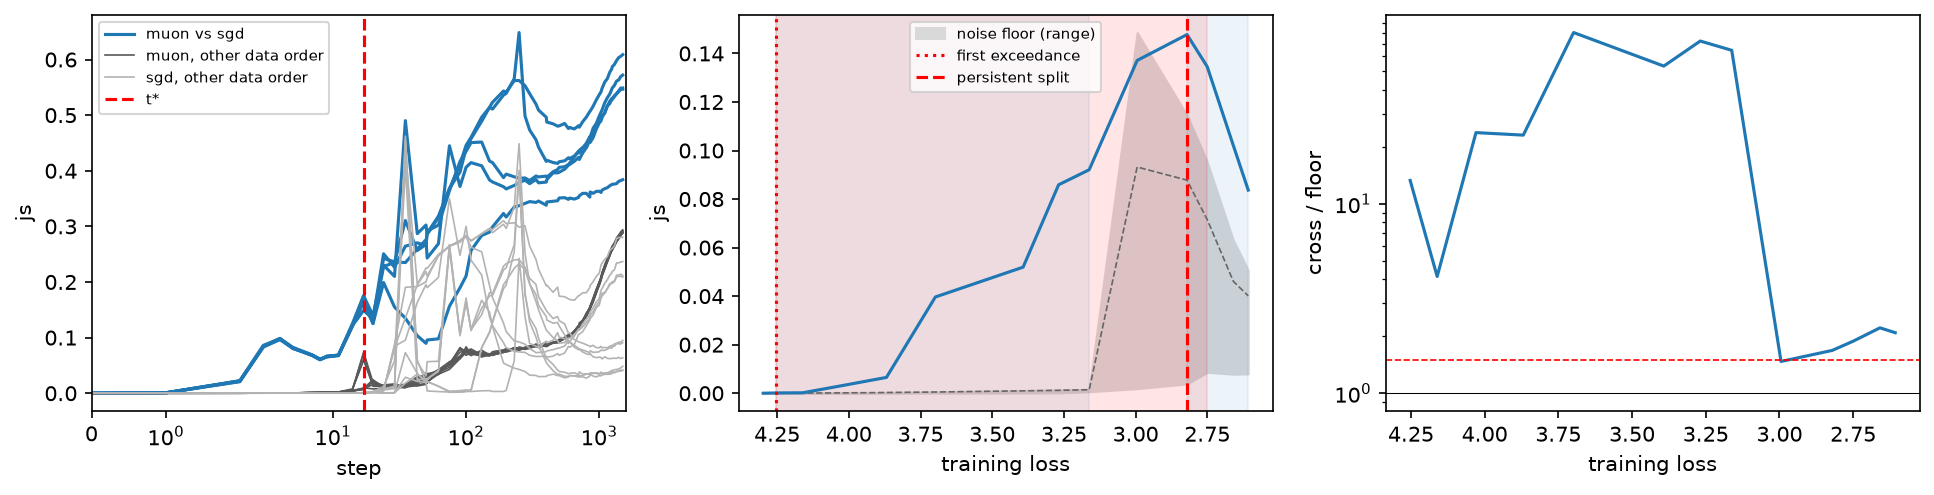
\includegraphics[width=0.9\linewidth]{figures/shakespeare/divergence_muon_sgd.png}
\caption{Function distance $D_\JS$ (bits) between optimizers. Rows: TinyStories-30M AdamW--Muon, Shakespeare
AdamW--Muon, Shakespeare Muon--SGD (the only persistent split). Left: by step, for the 5 cross pairs (blue,
same data order) and the 10 floor pairs of each optimizer (greys); the red line is the median step at which
the runs of the first optimizer reach the persistent split, or the first exceedance $t^\ast$ if there is none. Middle:
loss-matched distance (blue) against training loss (axis reversed), with the range over floor pairs (grey band),
the floor $F_\cD$ (dashed), the episodes above the floor (shaded), $t^\ast$ (dotted) and the persistent split
(dashed, with its 95\% interval shaded red). Right: cross distance over the floor, with the threshold
$1+m_\times=1.5$ (red). The other pairs are in \cref{fig:app-divergence,fig:app-divergence10}.}
\label{fig:divergence}
\end{figure}

\begin{table}[t]
\centering\small
\caption{Split analysis with $D_\JS$. Grid: range of the common loss grid. $t^\ast$: first exceedance
\eqref{eq:tstar}, found in 99.8\% of resamples (all those with at least two distinct data orders)
for every language-model pair but Matched--Muon, and in 52\% for CIFAR-10 (two data orders), with a 95\% interval equal to the point;
steps: the steps at which $A_0$ and $B_0$ reach it. Episodes: loss ranges above the floor. Persistent: the
persistent split $t^\ast_{\rm p}$ and the fraction of resamples in which one is found. Max and end: the ratio
$\bar c_\cD/F_\cD$ at its maximum and at the last grid level. ``Matched''\extra: Muon with its auxiliary AdamW
matched to AdamW (\cref{sec:setup}). Break-even rows compare plain SGD at two learning rates.}
\label{tab:tstar}
\setlength{\tabcolsep}{2.9pt}
\begin{tabular}{@{}llcccllcc@{}}
\toprule
Setting & Pair $A$--$B$ & Grid & $t^\ast$ & steps & Episodes\extra & Persistent\extra & Max & End \\
\midrule
Shakespeare & AdamW--Muon & 4.30--1.18 & 4.23 & 1 / 2 & 4.23--2.77, 2.30--2.12 & none (0\%) & 32 & 1.02 \\
            & AdamW--SGD  & 4.30--2.62 & 4.23 & 1 / 1 & 4.23--3.10 & none (34\%) & 98 & 1.69 \\
            & Muon--SGD   & 4.30--2.61 & 4.25 & 1 / 1 & 4.25--3.16, 2.82--2.61 & \textbf{2.82} (96.5\%) & 80 & 2.09 \\
            & Matched--AdamW & 4.30--1.19 & 4.26 & 1 / 1 & 4.26--2.85, 2.70--1.68 & none (0\%) & 29 & 1.07 \\
            & Matched--Muon & 4.30--0.23 & none (4\%) & -- & none & none (0\%) & 1.28 & 0.98 \\
TinyStories-10M & AdamW--Muon & 8.39--1.35 & 8.26 & 1 / 7 & 8.26--4.85 & none (0\%) & 111 & 0.99 \\
            & AdamW--SGD  & 8.39--2.04 & 8.26 & 1 / 3 & 8.26--6.32 & none (0\%) & 162 & 1.03 \\
            & Muon--SGD   & 8.39--2.02 & 8.38 & 1 / 1 & 8.38--5.81 & none (0\%) & 204 & 1.00 \\
TinyStories-30M & AdamW--Muon & 8.45--1.20 & 8.31 & 1 / 8 & 8.31--4.59 & none (0\%) & 124 & 1.02 \\
            & AdamW--SGD  & 8.45--1.65 & 8.31 & 1 / 2 & 8.31--6.03 & none (0\%) & 121 & 1.01 \\
            & Muon--SGD   & 8.45--1.65 & 8.44 & 1 / 1 & 8.44--6.82 & none (0\%) & 200 & 1.00 \\
\midrule
CIFAR-10 & $\eta$ 0.001--0.01 & 2.30--1.09 & 2.27 & 4290 / 510 & 4 short within 2.27--1.13 & none (0\%) & 19 & 1.47 \\
         & $\eta$ 0.01--0.1 & 2.30--0.0004 & 0.50 & 11310 / 2730 & 0.50--0.41 & none (0\%) & 1.75 & 1.24 \\
Shakespeare & $\eta$ 0.1--0.3 & 4.30--3.09 & none (0\%) & -- & none & none (0\%) & 1.17 & 0.72 \\
\bottomrule
\end{tabular}
\end{table}

\begin{figure}[t]
\centering
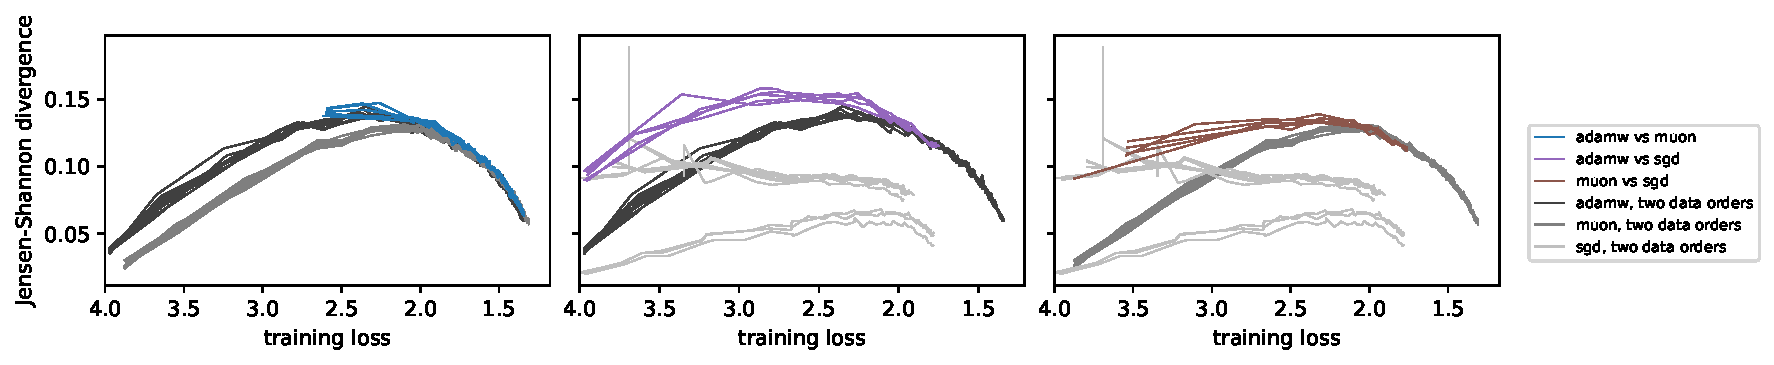
\includegraphics[width=\linewidth]{figures/ts10m/divergence_pairs.pdf}
\caption{TinyStories-10M: Jensen--Shannon divergence between two optimizers at equal training loss, for each data
order (colour), and between two data orders of the same optimizer (grey; one tone per optimizer). SGD's curves end
at its lowest training loss. Hyperparameters in \cref{tab:setup,tab:optim}.}
\label{fig:pairs}
\end{figure}

\begin{figure}[t]
\centering
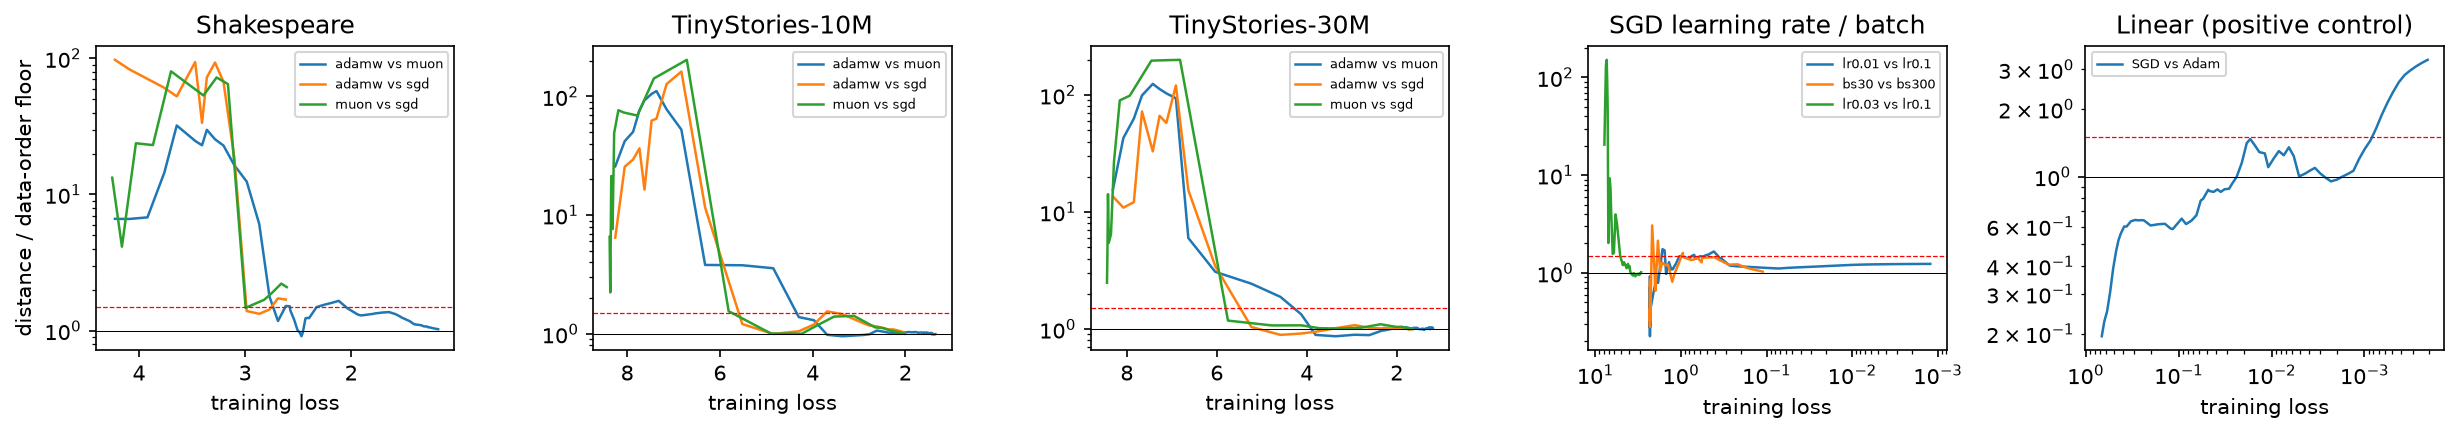
\includegraphics[width=0.85\linewidth]{figures/overview.png}
%% python scripts/overview_figure.py --panel Shakespeare split_adamw_muon.json ... --out overview.png
\caption{Function distance between two optimizers (or two SGD learning rates or batch sizes) at equal training
loss, over the distance between two runs of one of them with different data orders (training progresses to the
right). The red line is the threshold $1+m_\times=1.5$ of the split rule. In the language models the large ratios
at high loss lie within warmup, where the runs still share the initialization and the floor is near zero; after
warmup the ratio stays near 1, except for the pairs with SGD on Shakespeare, where SGD stalls (Muon--SGD is the
one persistent split). The learning rates and batch sizes of plain SGD on CIFAR-10 and TinyStories-10M (bottom
left) behave alike. Red, top left: AdamW--Muon trained to memorization (8000 steps\extra). Bottom middle: a linear
model on separable data, where gradient descent and Adam have different limits\extra; there the rule finds a
persistent split, near interpolation.}
\label{fig:overview}
\end{figure}

\Cref{tab:tstar} summarizes the split analysis for all pairs, \cref{fig:pairs} shows the loss-matched distances
of every pair on TinyStories-10M, \cref{fig:overview} the ratio to the floor in every setting, and
\cref{fig:divergence} three pairs in detail.

\paragraph{After warmup, about the floor.} After warmup, when their training loss is about the same, two runs
with different optimizers are about as far apart as two runs of one optimizer with different data orders
(\cref{fig:pairs}). For AdamW--Muon the ratio to the floor lies in 0.95--1.38 (median 1.02) below loss 4.85 on
TinyStories-10M, in 0.87--1.34 (median 1.01) below loss 4.59 on TinyStories-30M (both ranges include the end of
warmup), and in 1.02--1.46 (median 1.11) below loss 2.12 on Shakespeare, after a second, short episode
(2.30--2.12). On TinyStories the one exception is SGD on TinyStories-10M: it is up to about 1.5 times as far from
AdamW or Muon at losses 4--2.5 (1.3 times on average), not enough for an episode (\cref{tab:tstar}), and within
1.1 times below loss 2.5. On TinyStories-30M every pair stays within 1.1 times the floor after warmup. At the
lowest common loss all TinyStories pairs are at 0.99--1.03 times the floor. The largest absolute AdamW--Muon
distances, 0.14--0.15 bits near loss 2.3 on TinyStories, occur where the floor is as large (\cref{fig:pairs}).
On Shakespeare the pairs with SGD stay above the floor (below).

\paragraph{Within warmup, large ratios over a near-zero floor.\extra} The first exceedance $t^\ast$ is the first
or second level of the loss grid, reached at steps 1--8: two optimizers take different first steps while the
floor is still near zero. Each pair then has one long episode above the floor at high loss. It ends at loss
4.59--6.82 on TinyStories and 2.77--3.16 on Shakespeare, which the $d=0$ runs reach at steps 9--85, within warmup
in every pair but one (\cref{sec:res-coincide}), and the ratio peaks in it at 32--204. These ratios are inflated:
the runs still share their initialization, so the floor is near zero, and in absolute terms the cross distance in
the episode is at most 0.034--0.045 bits for AdamW--Muon and 0.04--0.18 bits for pairs with SGD. We report these
episodes as a detail of the first steps, not as a split.

\paragraph{One persistent split.\extra} Only Muon--SGD on Shakespeare has a persistent split: a second episode from
loss 2.82 to the end of the common grid at 2.61, found in 96.5\% of resamples (95\% interval 2.75--4.25). Muon
reaches it at steps 14--17 and SGD at steps 43--550, depending on the data order. This pair tells us the least
about how optimizers shape the function: the comparison stops at 2.61 because the slowest SGD run gets no
further, SGD at 0.05 is barely stable there (loss spikes, \cref{fig:losses}; erratic floor,
\cref{fig:divergence} bottom left), and four of its five runs end at training loss 2.32--2.58, about the
bigram level (the fifth at 1.66). AdamW--SGD on Shakespeare is borderline: after its episode the ratio stays at 1.33--1.73, which is a persistent split in
34\% of resamples but not in the full sample. On TinyStories SGD's own data-order noise is large (on
TinyStories-30M one run ends at validation loss 1.61 against 1.37--1.39 for the others; on TinyStories-10M the
runs end at 1.77--1.96), so ``no split'' against SGD means no larger than SGD's own data-order noise.

\paragraph{By step the picture differs.} At equal steps (left panels) the optimizers look different for much
longer, because they progress at different speeds: on TinyStories-30M Muon's loss stays flat for about the
first ten steps and then falls faster than AdamW's, and on Shakespeare Muon memorizes the training set while
AdamW does not (\cref{fig:losses}). \Cref{sec:res-route} separates the two effects for AdamW and Muon
(\cref{fig:div}).

\paragraph{Robustness.\extra} We repeated the estimate for every pair and setting with $D_{\rm dis}$ instead of
$D_\JS$, and with $D_\JS$ at $m_\times\in\{0.25,1\}$, $k\in\{2,5\}$ and $\tau\in\{0.01,0.05\}$, one change at a
time (seven variants). On both TinyStories models no variant finds a persistent split for any pair, nor
does any variant for AdamW and Muon on Shakespeare. The one persistent split, Muon against SGD on Shakespeare, is
fragile: it is found with $k=2$ (99\% of resamples), $m_\times=0.25$ and both tolerances, but not at the point
estimate with $D_{\rm dis}$, with $m_\times=1$ (26\% of resamples) or with $k=5$ (42\%). We read it as SGD ending
slightly off the others where it stalls, not as a clear split.

\subsection{AdamW against Muon, and optimizer against data order\extra}
\label{sec:res-route}

\paragraph{AdamW and Muon.} Muon is faster than AdamW (\cref{fig:div}, right). On TinyStories its loss is below
AdamW's at every logged step after warmup in every data order; on TinyStories-10M its training loss is 2.50
against 2.76 at step 250 and 1.77 against 1.95 at step 1000; and AdamW needs 1.35 (TinyStories-10M) and 1.22 times
(TinyStories-30M) as many steps to reach its own final validation loss. The speedup is in line with the 1.35 times
reported by \citet{jordan2024muon} and with \citet{wen2025fantastic}, and it does not come from a handicapped
AdamW: our Muon follows the reference implementation, only the learning rates were tuned, in the same way for
both, and the other difference is weight decay (none for Muon, 0.1 for AdamW; \cref{sec:setup}). Despite the gap
in loss, AdamW and Muon trained on the same data order stay close (\cref{fig:div}, left and middle): in the
embedding each such pair are nearest neighbours, and on TinyStories-10M their divergence at equal steps is
0--23\% below that between two data orders of one optimizer from step 250 to 3000, so at most about a fifth.
They are closer because they share their recent batches; at equal loss this vanishes (\cref{fig:pairs}).
Towards the end of training all six runs of \cref{fig:div} gather in one cluster, as their divergences shrink.

\begin{figure}[t]
\centering
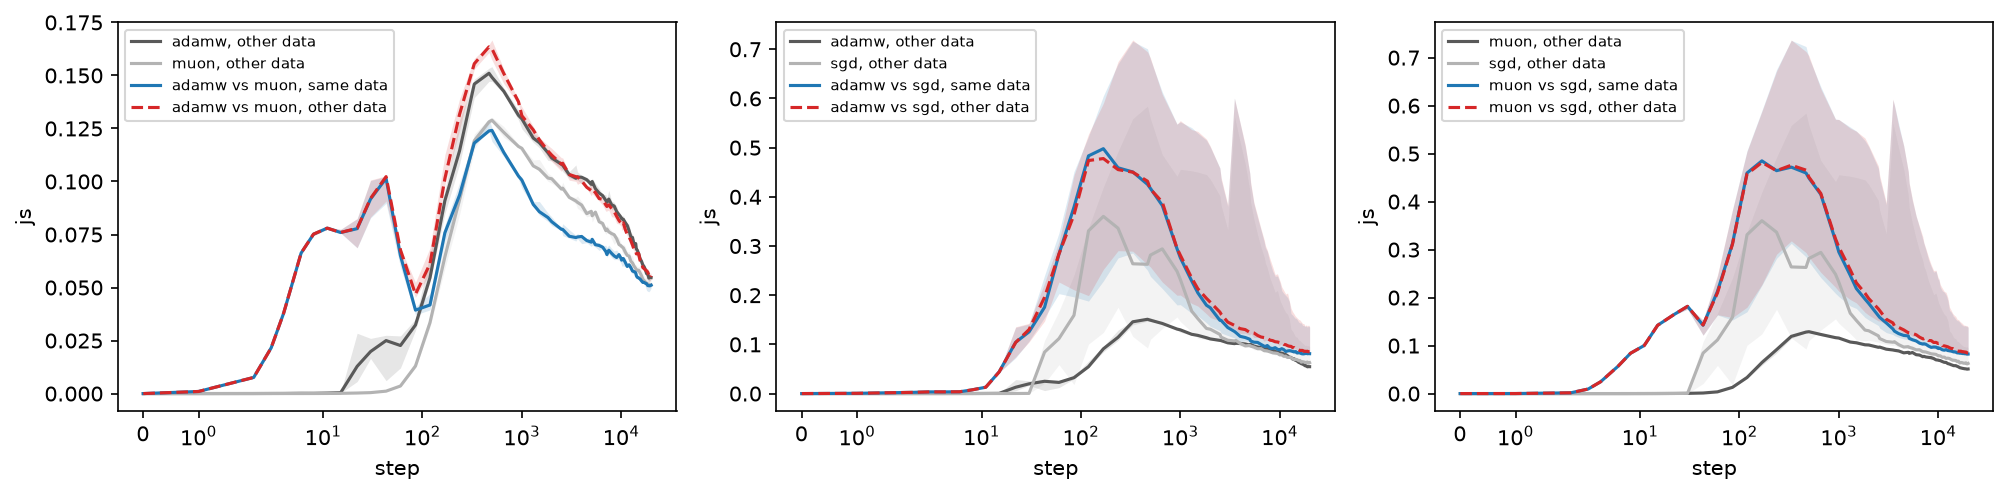
\includegraphics[width=\linewidth]{figures/ts30m/decompose_js.png}\\[2pt]
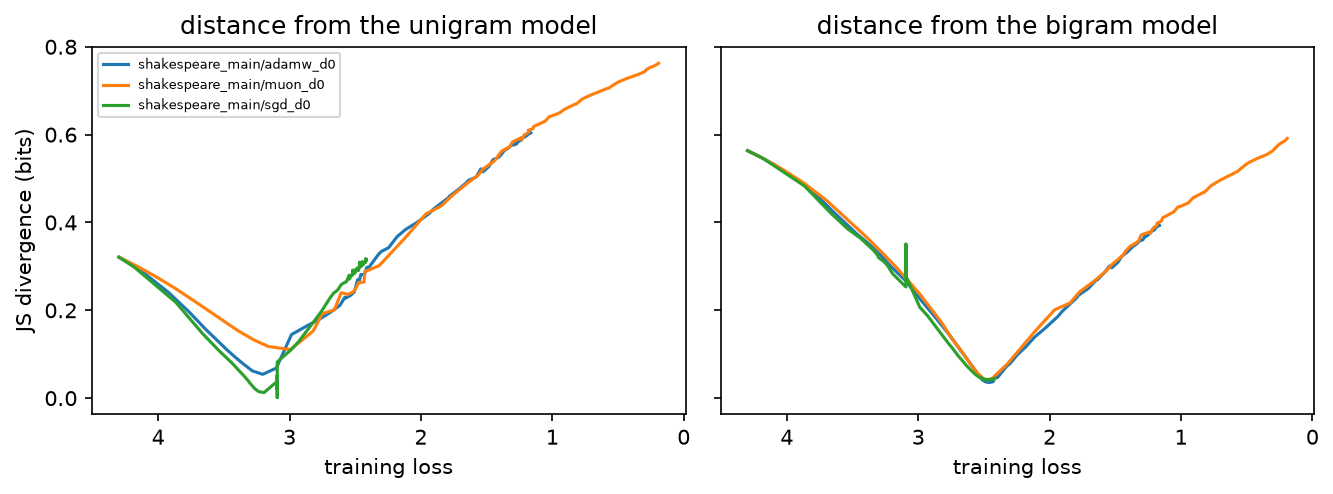
\includegraphics[width=0.6\linewidth]{figures/shakespeare/ngram.png}
\caption{Top: optimizer against data order at equal steps on TinyStories-30M (\cref{sec:method-route}): other
optimizer on the same data order (blue) and on another data order (red, dashed), and the two floors (greys);
median over the 5 data orders, range shaded. Bottom: $D_\JS$ of the $d=0$ runs on Shakespeare from the unigram
(left) and bigram (right) models of the training data, against training loss. Shakespeare decomposition and
TinyStories n-gram distances in \cref{fig:app-route}.}
\label{fig:route}
\end{figure}

\paragraph{Optimizer against data order.} On TinyStories-30M (\cref{fig:route}, top left), from step 332 on, the
AdamW--Muon distance on the same data order is at or below both optimizers' floors. At step 20{,}000 it is
0.051 bits, against floors of 0.055 (AdamW) and 0.051 (Muon) and 0.056 for AdamW and Muon on different data
orders: at the end of training, replacing AdamW by Muon changes the function no more than reshuffling the
data. Sharing the data order does keep the two optimizers closer: the same-data distance is 20--32\% below the
other-data distance between steps 119 and 10{,}000, and 8\% below at the end. Against SGD, the same-data
distances at the end are 0.081 (AdamW) and 0.082 bits (Muon), above the median floors (0.051--0.063), and
within 5\% of the other-data distances; at equal steps this includes SGD being slower (final validation loss
1.37--1.39, one run 1.61, against 1.18--1.20 for AdamW and Muon). On Shakespeare (\cref{fig:app-route}) the
optimizer dominates at equal steps: at step 1500 the AdamW--Muon distance is 0.26 bits, four times AdamW's
floor (0.06) but below Muon's own floor (0.29), which grows as Muon memorizes; same and other data orders give
the same distance (0.263 and 0.264).

\paragraph{N-gram stages.} On Shakespeare (\cref{fig:route}, bottom) the three optimizers pass close to the
bigram model at nearly the same training loss: the minimum distance to it is 0.036 (AdamW), 0.041 (Muon) and
0.041 bits (SGD), at loss 2.46, 2.47 and 2.48. At loss 2.47 the loss-matched AdamW--Muon ratio is 0.91. Before
that the routes differ: SGD passes through the unigram model (0.001 bits at loss 3.09) and AdamW near it
(0.054 at 3.20), while Muon stays further away (0.111 at 2.99). On TinyStories (\cref{fig:app-route}) the
optimizers come closest to the bigram model at loss 3.7--4.0, less closely than on Shakespeare (0.14--0.16 bits
for AdamW and Muon, 0.20 for SGD); the AdamW--Muon ratio stays below 1.2 from loss 3.69 (TinyStories-10M)
and 3.80 (TinyStories-30M) on. The episodes within warmup therefore cover the stage before the bigram
statistics are learned, where the optimizers take different routes while the data-order floor is still near
zero.

\subsection{What coincides with the changes in distance}
\label{sec:res-coincide}

\begin{figure}[t]
\centering
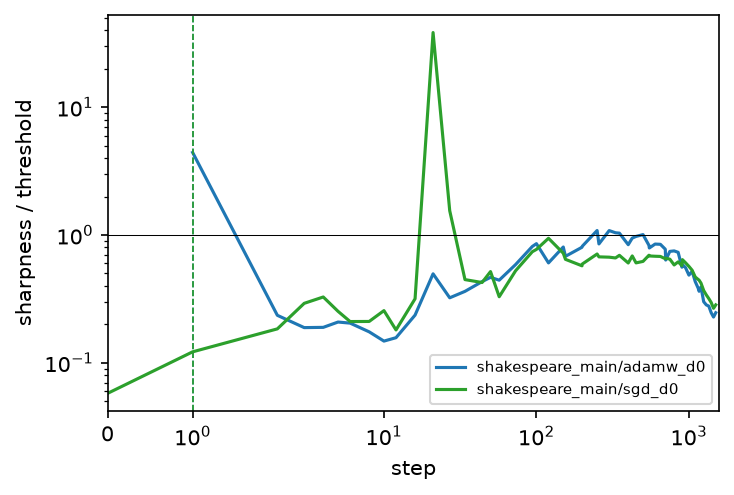
\includegraphics[width=0.325\linewidth]{figures/shakespeare/eos.png}\hfill
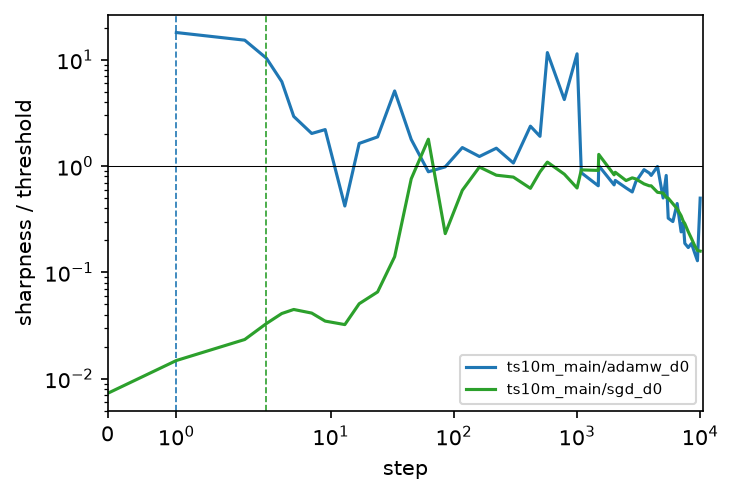
\includegraphics[width=0.325\linewidth]{figures/ts10m/eos.png}\hfill
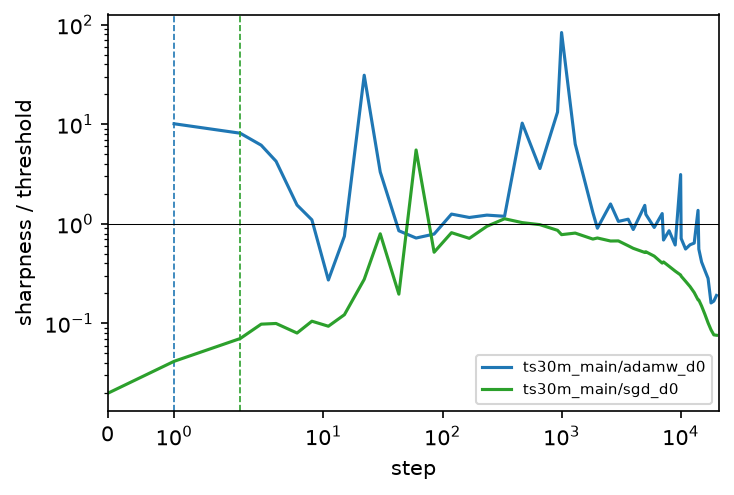
\includegraphics[width=0.325\linewidth]{figures/ts30m/eos.png}\\[2pt]
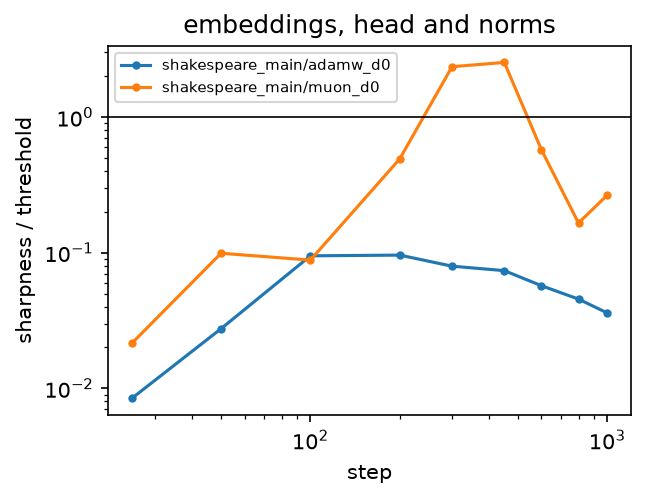
\includegraphics[width=0.3\linewidth]{figures/shakespeare/aux_eos.png}\qquad
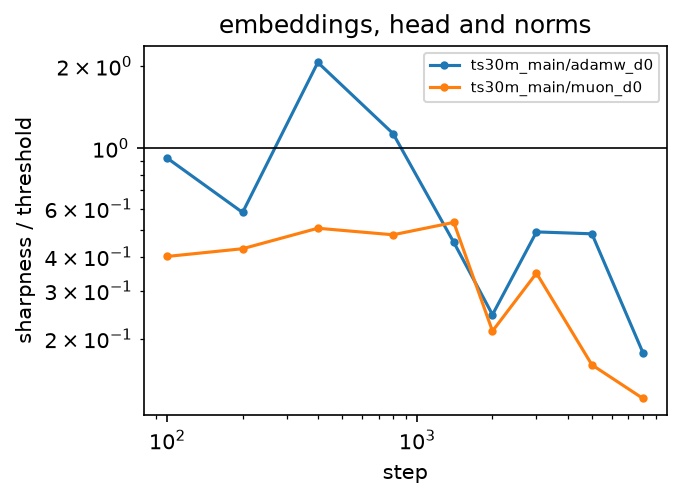
\includegraphics[width=0.3\linewidth]{figures/ts30m/aux_eos.png}
\caption{Top: sharpness over its stability threshold for the $d=0$ runs on Shakespeare, TinyStories-10M and
TinyStories-30M: $\lmax\,\eta_s/(2+2\mu)$ for SGD and the preconditioned sharpness times
$(1-\beta_1)\eta_s/(2+2\beta_1)$ for AdamW; 1 is the edge of stability, dashed lines the first exceedance
$t^\ast_X$ of the AdamW--SGD pair. Bottom\extra: the same ratio for the embeddings, head and gains alone
(\cref{sec:method-aux}), at the fork checkpoints of AdamW and Muon, on Shakespeare (left) and TinyStories-30M
(right). Raw sharpness, batch sharpness and thresholds in \cref{fig:app-sharpness}.}
\label{fig:sharpness}
\end{figure}


\paragraph{SGD} reaches its threshold $(2+2\mu)/\eta_s$ only early in training, around and after the end of warmup (\cref{fig:sharpness};
\cref{tab:coincide} in \cref{app:figures}): in the $d=0$ runs $\lmax$ is within 10\% of it, or above, only between steps 21 and 120,
62 and 1500, and 60 and 658, for warmups of 100, 200 and 400 steps, and at 2--16\% of the measured steps over all data orders.
After that, $\lmax$ levels off and does not follow the threshold, which rises as the learning rate decays: the
threshold is a ceiling, and the runs leave the edge of stability once the decay sets in. On Shakespeare the SGD
runs have large transient spikes (maximum ratio 7.9--956 over the data orders), matching their loss spikes.
Batch sharpness stays below $\lmax$, and so below the threshold, apart from early transients
(\cref{fig:app-sharpness}).

\paragraph{AdamW.} The preconditioned sharpness is above its threshold at the first measured steps (ratio 3
to 21 at step 1), when the second-moment estimate rests on one or a few gradients, so $s_{\rm EoS}=1$ in every
run. After a dip it returns to the threshold or above (on TinyStories-30M with spikes to 10--80 times it around
steps 500--1000) and stays there for long stretches, until the cosine decay
raises the threshold away from it: the ratio is at least 0.9 at measured steps up to 425--600 of 1500 on
Shakespeare, 4500--9500 of 10{,}000 on TinyStories-10M and 9000--19{,}000 of 20{,}000 on TinyStories-30M
(11--16\%, 50--65\% and 40--69\% of the measured steps). This is the adaptive edge of stability of
\citet{cohen2022adaptive}.

\paragraph{Muon.} Its threshold applies to a spectral-norm sharpness that we have not yet measured
(\cref{sec:method-sharpness}); of its $\lmax$ we only note that it fluctuates widely on Shakespeare (between
about 10 and 400) and is smooth on TinyStories (\cref{fig:app-sharpness}).

\paragraph{Across learning rates.\extra} In the sweeps with sharpness measurements
(\cref{sec:method-sharpness}) the plateau of the sharpness falls about as $1/\eta$ for all three optimizers. On
TinyStories-10M the log-log slope against the peak rate is $-0.96$ for SGD (3 rates, at 0.8--0.9 of its
threshold), $-0.73$ for AdamW's preconditioned sharpness (3 rates, at 1.0--1.5 of its threshold) and $-0.86$ for
its raw $\lmax$, and $-0.84$ for Muon's raw $\lmax$ (4 rates). On Shakespeare AdamW's slope is $-0.90$, at its
threshold, without its two largest rates, which blew up; SGD stalls at loss 2.5 at every rate, so its sweep says
nothing; and Muon's slope is $-0.21$ over four rates but $-1.0$ over the three smallest. As in the main runs, the
sharpness levels off after warmup and does not follow the threshold up as the cosine decay lowers the rate.
Muon's $\lmax(H)$ thus scales like the thresholds of the other two, although its own threshold is on a
spectral-norm sharpness (\cref{sec:theory}). Unlike \citet{jastrzebski2020breakeven}, who keep the learning
rate constant, these runs use warmup and cosine decay to 10\%; our CIFAR-10 replication uses a constant rate, as
they do (\cref{sec:res-breakeven}).

\paragraph{Coincidences.} No edge-of-stability event explains the changes in distance. The first exceedance,
at steps 1--8, comes before the end of warmup and before SGD's onset; it coincides only with AdamW's onset at
step 1, which reflects the preconditioner of the first steps rather than an edge of stability. The early
episodes are short in steps: the $d=0$ runs reach the loss at which the episode ends at steps 9--85 (221 for SGD in
the TinyStories-10M Muon--SGD pair), within warmup in every pair but that one. For the pairs with SGD this is at
SGD steps 20--45 (and 221), in the same range as SGD's onset in the $d=0$ runs (steps 21, 62 and 60). But the
AdamW--Muon pairs return to the floor in the same way without SGD, and AdamW, which reaches that loss at steps
29, 45 and 60, stays near its threshold long after the distance has returned to the floor. At the one persistent
split (Muon--SGD, Shakespeare), each SGD run is below its threshold when it reaches loss 2.82 (ratio
0.18--0.80), and Muon's auxiliary AdamW is far below its own (ratio 0.02 at step 25, the first fork checkpoint
after Muon reaches 2.82). As a loss level the end of the early episode is similar across the two TinyStories
sizes (AdamW--Muon: 4.85 and 4.59) and close to the bigram stage (\cref{sec:res-route}), which suggests
describing it as a stage of learning rather than a step.

\paragraph{The block left to Muon's auxiliary AdamW.\extra} On Shakespeare (\cref{fig:sharpness}, bottom left), the
embeddings, head and gains of Muon exceed their threshold at the fork checkpoints at steps 300 and 450 (ratio
2.35 and 2.53) and are below it at the other seven (at most 0.57), while in the AdamW run the same block stays
at most 0.10 times its threshold. These steps come just before Muon's validation loss starts to rise, and in
this period Muon's top Hessian eigenvector lies almost entirely in the embeddings (\cref{sec:res-anatomy}). On
TinyStories-30M it is the other way round: AdamW's block exceeds its threshold at steps 400 and 800 (2.06 and
1.13) and Muon's stays at most 0.53. In both settings the block that overshoots is trained by the Adam with the
larger learning rate on these parameters (Shakespeare: Muon's $10^{-3}$ against AdamW's $3\cdot10^{-4}$;
TinyStories-30M: AdamW's $2\cdot10^{-3}$ against Muon's $1.5\cdot10^{-3}$), so the learning rate plays a
role; the control below shows that it is not the whole story.

\paragraph{Control.\extra} Matching Muon's auxiliary AdamW to AdamW (\cref{sec:setup}) does not remove the
memorization: matched Muon still reaches training loss 0.22 with validation loss 2.5, against 1.55 for AdamW,
so the memorization comes from Muon's updates of the hidden matrices. With the same Adam, learning rate and
threshold on the embeddings, head and gains as AdamW, matched Muon's block still reaches its threshold (ratio 1.14
and 1.08 at steps 600 and 1000, against at most 0.10 for AdamW; \cref{fig:app-auxeos}), later and less far than
with Muon's default $10^{-3}$ (2.35 and 2.53 at steps 300 and 450). Its raw sharpness on this block reaches
236 and 579 at steps 600 and 1000, against at most 61 for AdamW. So Muon's updates of the hidden matrices make the embeddings sharper, and the
larger learning rate of the default auxiliary AdamW brings the overshoot forward. In function space matched Muon is
indistinguishable from Muon (first exceedance in 4\% of resamples, ratio at most 1.28; \cref{tab:tstar}), and
against AdamW it behaves as Muon does: two episodes (4.26--2.85 and 2.70--1.68), no persistent split, and a
ratio of 1.07 at the lowest common loss (\cref{fig:app-divergence}).

\subsection{Swaps and mode connectivity}
\label{sec:res-swap}

\begin{figure}[t]
\centering
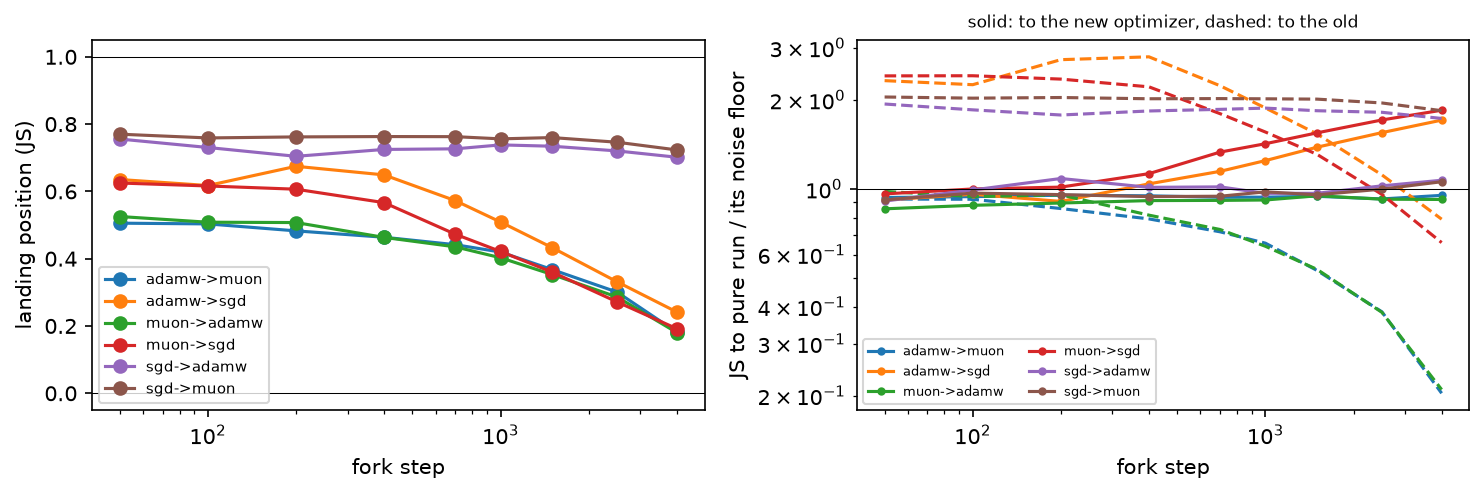
\includegraphics[width=0.75\linewidth]{figures/ts10m/swap.png}\\[2pt]
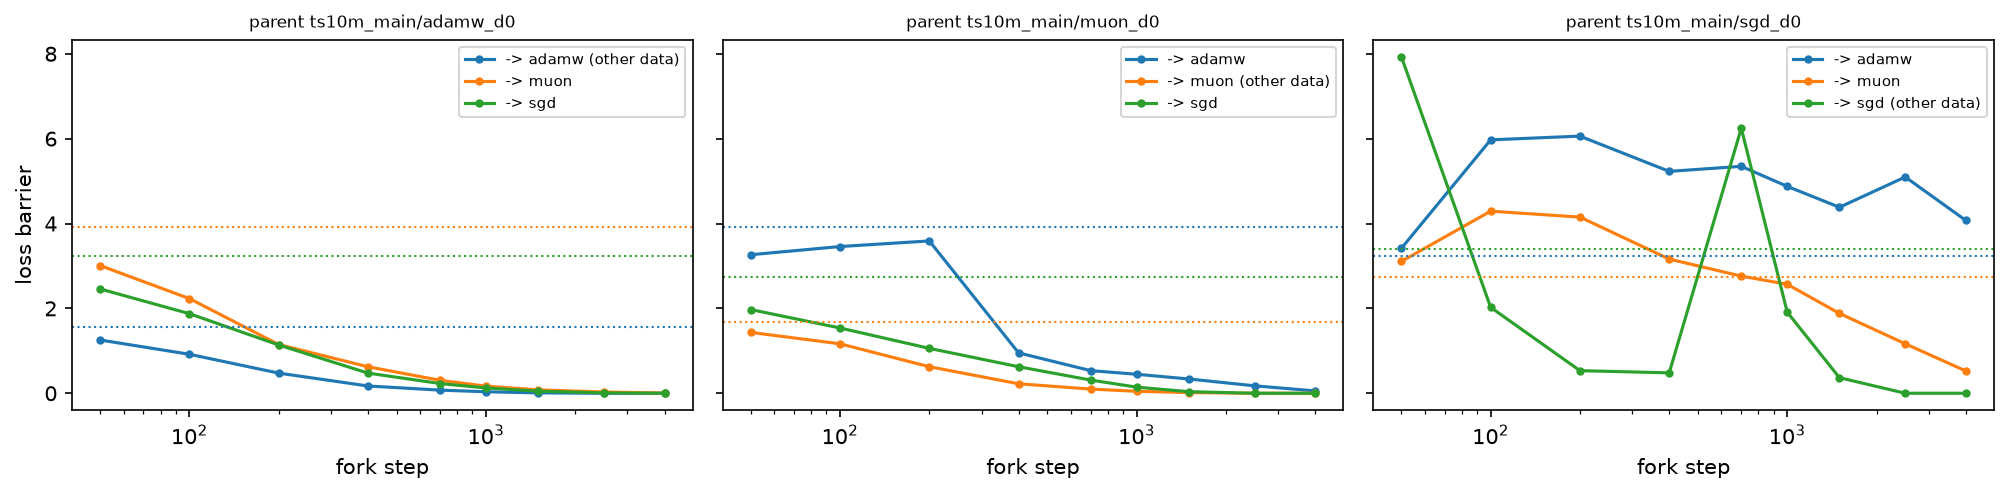
\includegraphics[width=\linewidth]{figures/ts10m/lmc.png}
%% python -m optsplit.analysis.swap --forks 'ts10m_forks/*' --pure 'ts10m_main/*' --out swap
%% python -m optsplit.analysis.plots swap --swap-json swap.json
%% python -m optsplit.analysis.lmc --parent ts10m_main/adamw_d0 --forks 'ts10m_forks/adamw_to_*' --others 'ts10m_main/*_d0' ts10m_main/adamw_d1 --out lmc_adamw.json
%% python -m optsplit.analysis.plots lmc --lmc-json lmc_adamw.json lmc_muon.json lmc_sgd.json
\caption{Swaps and mode connectivity on TinyStories-10M. Top left: landing coordinate $r$
\eqref{eq:landing} with $D_\JS$ against the fork step, for the six ordered pairs; 0 is the final function of the
parent (optimizer kept), 1 that of the pure run of the new optimizer (same batches). Top right\extra: the fork's
distance to the pure run of the new optimizer (solid) and of the old one (dashed), each over that pure run's
final data-order floor. Bottom: barrier \eqref{eq:barrier} between the final weights of each $d=0$ parent and of
its forks against the fork step; ``other data'' are the forks that keep the optimizer and change the data
order. Dotted\extra: barrier to the pure runs of the other optimizers and to the parent's optimizer with data order
1, which share only the initialization.}
\label{fig:swap}
\end{figure}

\paragraph{Swaps.} On TinyStories-10M (\cref{fig:swap}, top) the forks fall into three groups.
\emph{AdamW$\leftrightarrow$Muon}: at every fork step from 50 to 4000 the fork ends within the floor of the
pure run of the new optimizer (0.86--0.95 floors) and, increasingly with the fork step, also of the parent's
(0.92 floors at step 50, 0.20 at step 4000), so $r$ falls from 0.5 to 0.18. Since the two pure runs are
themselves within the floor of each other at the end (\cref{sec:res-route}), these swaps cannot reveal an
imprint of either optimizer. \emph{SGD$\to$AdamW and SGD$\to$Muon} land on the new optimizer (0.91--1.08 floors
from its pure run) at every fork step up to 4000, and stay 1.7--2.0 floors from pure SGD: 4000 steps of SGD
leave no trace that AdamW or Muon do not erase. \emph{AdamW$\to$SGD and Muon$\to$SGD} land on pure SGD when
forked by step 200 (0.91--1.01 floors); later forks end further from it (1.04--1.42 floors at steps 400--1000),
and from step 1500 on closer to the parent than to pure SGD (0.66--0.79 floors from the parent and 1.7--1.8 from
pure SGD at step 4000): SGD at its stable rate is too slow to undo what the
adaptive optimizer has already learned. In function space the last optimizer decides the endpoint whenever it
is fast enough to do so, and none of the forks keeps an imprint of an early phase that the later optimizer
could have reached on its own. Nearly all fork steps lie after the end of the early episodes (steps 9--85 in the
$d=0$ runs, \cref{sec:res-coincide}), and $r$ changes smoothly across them, so the end of the episode does not
decide the endpoint either.

On Shakespeare (\cref{fig:app-swap}) the same rule holds, with Muon as the fast optimizer. AdamW$\to$Muon and
SGD$\to$Muon land on pure Muon (0.93--1.05 floors) at every fork step from 25 to 1000. The reverse swaps do not
land on the slower optimizer: from step 50 on, forks from Muon into SGD stay with Muon (0.43--1.03 of Muon's
floor, 5.7--9.0 of SGD's), and forks from Muon into AdamW end 1.2 floors from pure AdamW at step 25 but 3.2 at
step 1000. Muon's floor is large here (0.29 bits, against 0.06 for AdamW), as its runs memorize different
things, so ending within it is a weak statement. Forks from SGD into AdamW keep a mark of SGD from step 50 on
(3.2--5.7 floors from pure AdamW): AdamW at $3\cdot10^{-4}$ does not undo the early, unstable phase of SGD on
Shakespeare in the remaining steps. Forks from AdamW into SGD are erratic ($r$ between 0.01 and 0.93), like
SGD's own runs there. In both settings, then, the optimizer that trains last decides the function when it
is fast enough to undo the earlier optimizer's work in the remaining steps: on TinyStories whenever it is the
faster one, and otherwise only for early forks.

\paragraph{Mode connectivity.} Forks that keep the optimizer and change the data order
(\cref{fig:swap}, bottom) become linearly connected to their parent at about the same time for AdamW and Muon:
the barrier falls below 0.05 nats for forks from step 1000 (AdamW 0.035, Muon 0.046) and to 0 from step 2500,
the stability point of \citet{frankle2020lmc} at 10--25\% of training. For SGD the same barrier jumps between 0.4
and 7.9 up to step 1500, like its data-order noise (\cref{sec:res-split}), and is 0 from step 2500. A change of optimizer needs a later
fork to stay in the parent's basin: from the AdamW parent the Muon and SGD forks reach 0.03 and 0.01 nats only at
step 2500, from the Muon parent the AdamW fork is still at 0.055 at step 4000, and from the SGD parent the AdamW
fork is never connected (barrier 3.4--6.1 at every fork step) and the Muon fork only approaches it (0.53 at step
4000). Weight space thus keeps a mark of the optimizer that function space does not: the fork from AdamW to Muon
at step 1000, which ends within the floor of both pure runs, has a barrier of 0.17 to its parent, against 0.035
for the fork that keeps AdamW and changes the data order. The pure runs, which share only the initialization, are
not linearly connected for any pair (dotted lines); we compare them below.

On Shakespeare (\cref{fig:app-swap}, bottom) the forks that keep AdamW and change the data order are connected
to their parent from step 300 on (0.015, then 0), and even the pure AdamW runs with two data orders have
barriers of only 0.11--0.17: at $3\cdot10^{-4}$ AdamW stays close to the initialization. Forks from AdamW into Muon or
SGD keep barriers of 1.4--3.3 up to step 600, and those into Muon are still at 0.27 at step 1000; forks from SGD
into Muon stay at 1.3--1.7 up to step 800. The exception is the Muon parent: its forks with another data order
are connected only from step 800 (barrier 3.5 at step 25, 0.06 at 800), later than its forks into AdamW and SGD
(0.9 and 0.7 at step 100, 0.01 at 800). Muon on Shakespeare is unstable to the data order for half of training,
while it memorizes, and its forks into slower optimizers move the weights less after the fork. Apart from this
case, a fork that changes the optimizer stays further from its parent in weight space than one that changes
the data order, although it does not in function space.

\paragraph{Do swaps end in the new optimizer's basin?\extra} A fork into $B$ that ends at $B$'s function need not end
in the region of weight space of the pure $B$ run. We computed the barrier between the final weights of each pure
$d=0$ run and of every fork into its optimizer (\cref{fig:app-lmc-into}). On TinyStories-10M the forks into AdamW
(2.9--8.0 nats) and into Muon (3.5--6.5) are further from the pure run than the same optimizer with another data
order from the initialization (1.2--1.9 and 1.6--1.8 over ten pairs), at every fork step from 50 on, while the
forks into SGD (2.4--3.4) are within SGD's own data-order barriers (0.1--4.1). The forks from AdamW into Muon, for instance, end within Muon's
data-order floor in function space at every fork step, but 3.7--4.3 nats of barrier away from pure Muon. On
Shakespeare the forks into AdamW (0.8--2.4) are far above AdamW's data-order barriers (0.11--0.17), while those
into Muon (2.3--6.6) and SGD (0.9--2.3) are comparable to Muon's (3.6--6.6) and SGD's (1.0--3.2). As few as 50 steps of another
optimizer at the start can move the endpoint further in weight space than a different order of all the data,
while in function space they leave no trace.

\paragraph{TinyStories-30M.} The larger model (\cref{fig:app-swap-30m,fig:app-lmc-into}) repeats these results,
with one difference in the swaps into SGD. Forks between AdamW and Muon end within the floor of both pure runs at
every fork step from 100 to 8000 (of 20{,}000), and $r$ falls from 0.52 to 0.25. Forks from SGD land on the new
optimizer (0.84--1.07 floors) at every fork step, but pure SGD ends only 1.1--1.4 floors from AdamW and Muon here,
so these swaps say little. Forks from AdamW and Muon into SGD land near pure SGD up to step 3000 (0.92--1.21
floors), and only those at steps 5000 and 8000 end closer to the parent (0.57--1.00 floors from it) than to pure SGD,
against step 1500 on TinyStories-10M: SGD's tuned rate is higher here (0.1 against 0.03), so it erases more. Forks that keep
AdamW or Muon and change the data order are connected to their parent from step 2000 (0.022 and 0.040 nats, 0 from
step 5000). Those that keep SGD have a barrier of only 0.14 at step 100 and below 0.06 from step 400, although the
pure SGD runs with data orders 0 and 1 have a barrier of 8.8: SGD's sensitivity to the data order is confined to the
first 100 steps. A change of optimizer again needs a later fork. From AdamW the SGD fork reaches 0.048 nats at
step 3000, and the Muon fork 0.077 only at step 8000. From Muon the SGD fork is connected from step 3000 (0.068),
but the AdamW fork is still at 0.19 at step 8000. From SGD the AdamW and Muon forks are never connected (0.69 and
0.29 at step 8000). The forks into Muon (4.4--5.7 nats) again end further from the pure run than another data order
does (1.6--2.1), at every fork step. The forks into AdamW (3.5--18.8) do so only when forked at steps 200--400 from
Muon and 200--5000 from SGD, since AdamW's own data orders are 3.3--6.8 nats apart here, and the forks into SGD
(1.6--2.9, apart from 10.2 for Muon at step 100) stay within SGD's own (0.6--9.2).

\begin{figure}[t]
\centering
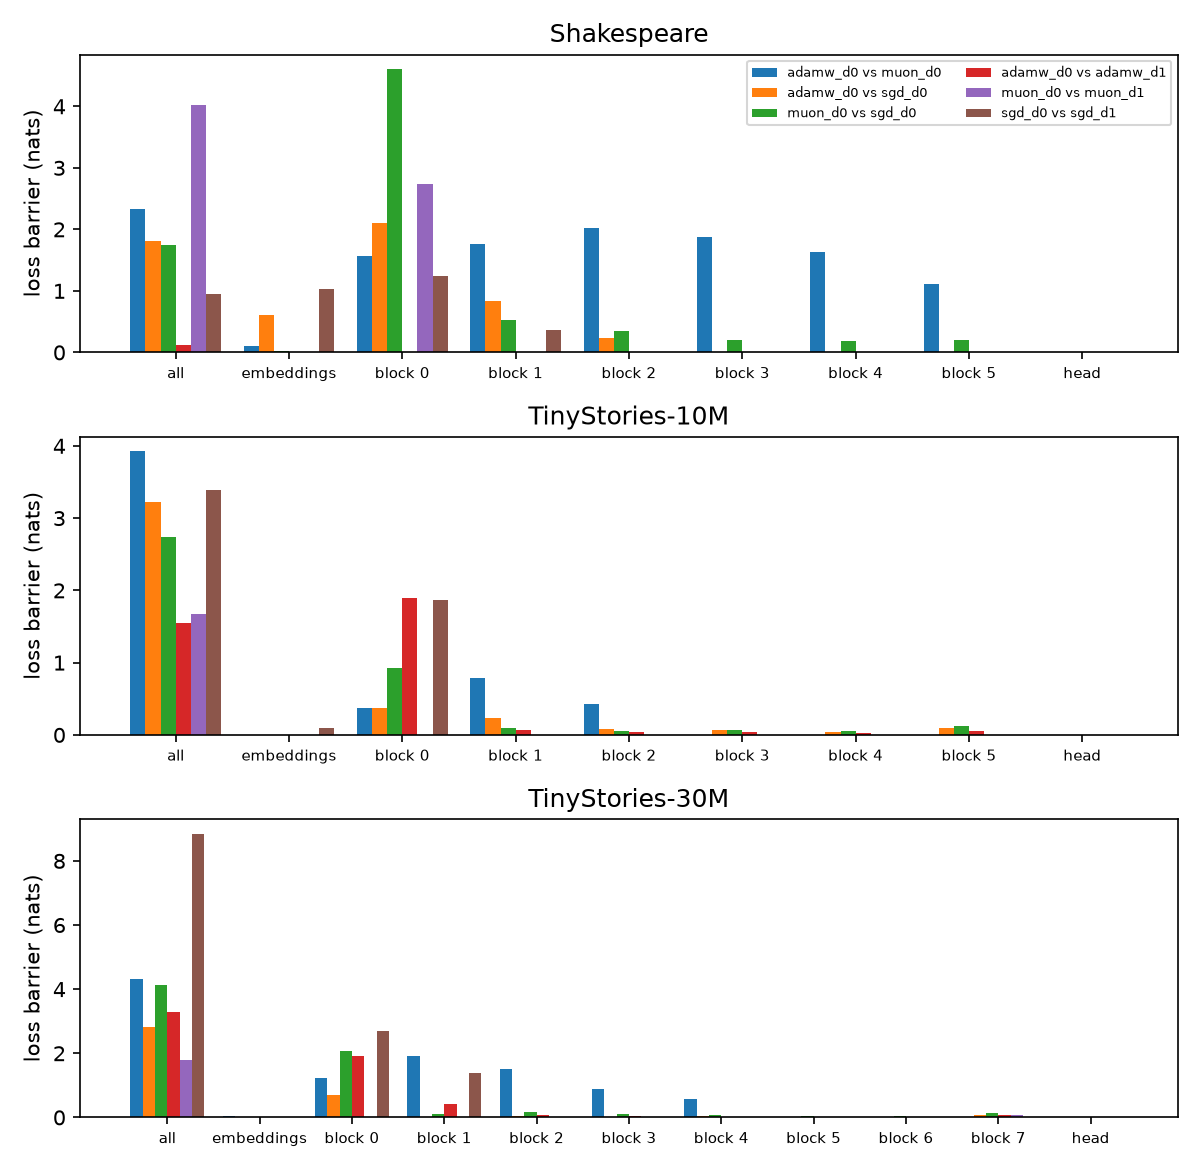
\includegraphics[width=0.85\linewidth]{figures/lmc_layers.png}
%% bash lmc_pairs.sh S {cross,adamw,muon,sgd}; python -m optsplit.analysis.lmc_layers --plot T=S/pairs_cross/lmc_layers.json,... --out .
\caption{Loss barriers\extra\ between the final weights of pure runs, for every pair that differs only in the optimizer
(5 per pair of optimizers) or only in the data order (10 per optimizer); mean and standard deviation over pairs.
``All'' is the ordinary barrier; for the other groups only that group of parameters moves along the straight line
from the first run to the second, the rest stay at the first run's \citep{adilova2024layerwise}.}
\label{fig:lmc-layers}
\end{figure}

\paragraph{Barriers between pure runs\extra.} We computed the barrier between the final weights of every pair of
pure runs that differ only in the optimizer or only in the data order, in full and with one group of parameters
moved at a time (\cref{fig:lmc-layers}). In size, a change of optimizer is not consistently further than a change
of data order. AdamW and Muon are further apart than two data orders of either on TinyStories-10M (3.5--4.1 nats
against 1.2--1.9 and 1.6--1.8), but not on TinyStories-30M, where AdamW's data orders are 3.3--6.8 nats apart
(AdamW--Muon 4.3--4.8), nor on Shakespeare, where Muon's are 3.6--6.6 apart (AdamW--Muon 2.1--2.7); SGD's
data-order barriers vary so much (0.1--4.1 and 0.6--9.2 on TinyStories) that the pairs with SGD fall within them.
Where the barrier sits does tell them apart. Between two data orders the single-layer barriers sit in the first
block, up to 4.0 nats on average, and are at most 0.6 in any later block, or there are none at all (AdamW on
Shakespeare, Muon on TinyStories-30M) although the full barrier is not small. Between AdamW and Muon on the same
data they extend into the middle of the network: 0.8 and 0.4 nats in blocks 1--2 on TinyStories-10M, 2.3--0.5 in
blocks 1--4 on TinyStories-30M and 1.1--1.9 in blocks 1--5 on Shakespeare. The pairs with SGD look like data
orders, with the barrier mostly in the first block (and the embeddings on Shakespeare), and the head carries none
(the loss is convex in the head). Two data orders, or SGD and an adaptive optimizer, thus end in solutions that
differ in how the first block reads the embeddings, while AdamW and Muon also differ in how the middle blocks
process them.

\subsection{Anatomy of the sharp direction}
\label{sec:res-anatomy}

\begin{figure}[!htb]
\centering
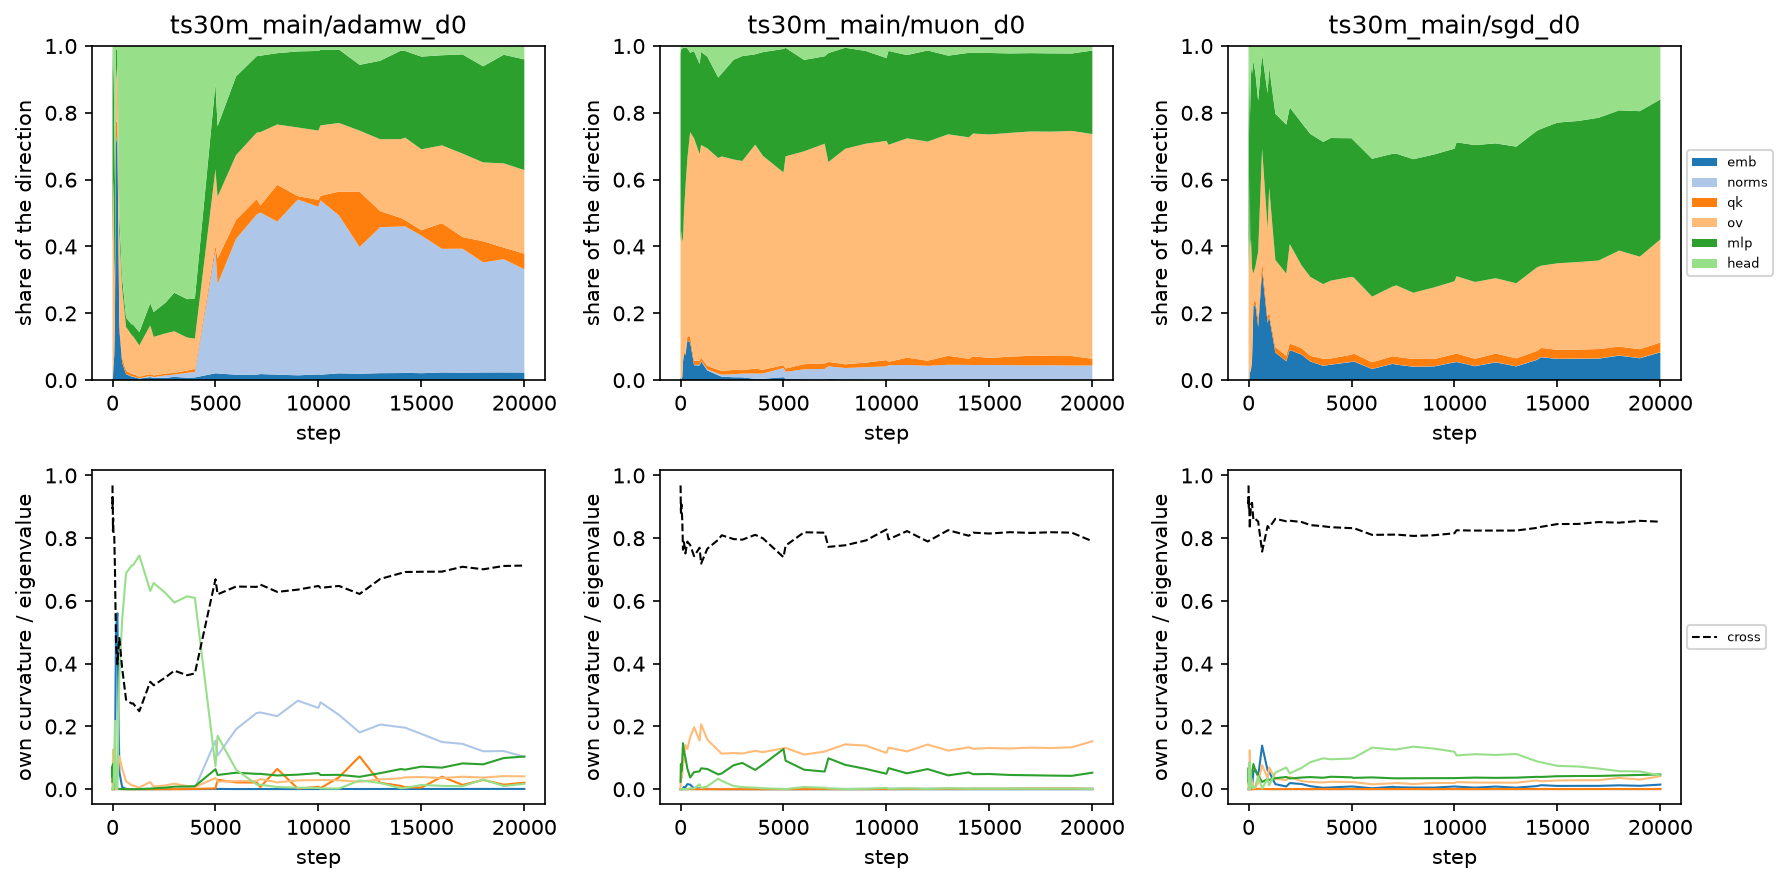
\includegraphics[width=0.62\linewidth]{figures/ts30m/anatomy.png}
\caption{Anatomy of the top Hessian eigenvector of the $d=0$ runs on TinyStories-30M \eqref{eq:anatomy}. Top:
share of the direction $\|v_b\|^2$ by block type. Bottom: each block type's own curvature $s_b$ and the
cross-block remainder $\chi$ (dashed), as fractions of the eigenvalue. Shakespeare and TinyStories-10M in
\cref{fig:app-anatomy}.}
\label{fig:anatomy}
\end{figure}

On TinyStories-30M (\cref{fig:anatomy}) the sharp direction differs by optimizer. Muon's lies mostly in the
value--output matrices (about 60--70\% of the direction) throughout training, with most of the rest in the
MLP matrices. AdamW's lies in the head until about step 4000 and then largely in the gains (30--50\%), with the
value--output and MLP matrices. SGD's is spread over the MLP, value--output and head blocks. In all three the
cross-block term $\chi$, which here also counts the curvature between the attention and MLP matrices of one
layer, is the largest part of the eigenvalue: about 75--85\% for Muon and SGD throughout, and
for AdamW about 25--40\% while the head dominates and 60--70\% after. The sharp direction is therefore not the
top eigenvector of a single block but comes from curvature between blocks. On TinyStories-10M
(\cref{fig:app-anatomy}) Muon's direction is again in the value--output matrices (60--70\%), while AdamW's stays
mostly in the head (60--75\%). On Shakespeare Muon's direction lies almost entirely (85--97\%) in the
embeddings from step 200 on, with the embeddings' own curvature making up most of the eigenvalue: the sharp
direction is in the block that Muon leaves to its auxiliary AdamW, including the period in which that block
is over its threshold (\cref{sec:res-coincide}). AdamW's direction on Shakespeare is spread over the MLP,
value--output and embedding blocks, with about 70\% of the eigenvalue from $\chi$. The changes of dominant
block (AdamW on TinyStories-30M, head to gains around step 4000--5000) happen long after warmup, when the
loss-matched distance between optimizers is at the floor. For AdamW the top eigenvector of the preconditioned\extra
operator $P^{-1/2}HP^{-1/2}$, the one that sets its stability threshold, lies elsewhere than that of $H$
(\cref{fig:app-anatomy-precond}): mostly in the MLP matrices (40--60\%), the attention matrices and the
embeddings on both TinyStories sizes, rather than in the head or the gains, with short periods (the first 1000
steps and a few isolated measurements) in which it lies almost entirely in the embeddings and their own curvature
makes up the eigenvalue. Outside those periods 80--95\% of the preconditioned eigenvalue comes from curvature
between blocks, even more than for $H$.

\begin{figure}[!htb]
\centering
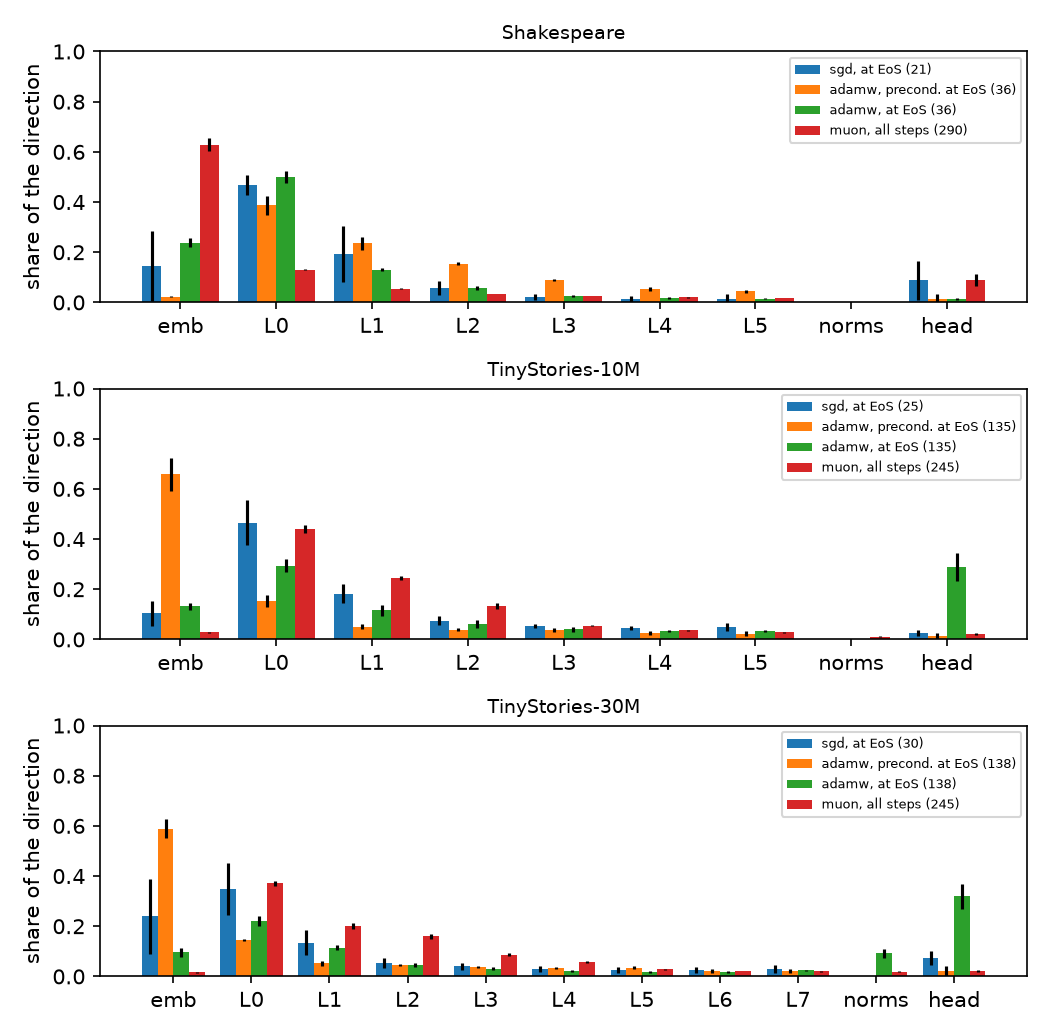
\includegraphics[width=0.68\linewidth]{figures/anatomy_layers.png}
%% python -m optsplit.analysis.anatomy_layers 'ts10m_main/*' --out analysis/ts10m (per setting), then
%% python -m optsplit.analysis.anatomy_layers --plot Shakespeare=... TinyStories-10M=... TinyStories-30M=... --out report/figures
\caption{Share of the top eigenvector by layer at the edge of stability (sharpness at least 0.9 of the threshold),
mean and standard deviation over the five data orders; in brackets, the number of measured steps. For AdamW,
of $P^{-1/2}HP^{-1/2}$ (which sets its threshold) and of $H$ at the same steps; for Muon, of $H$
(threshold: spectral-norm sharpness), all steps. L$i$: transformer block $i$; norms: the gains of all LayerNorms.}
\label{fig:anatomy-layers}
\end{figure}

\paragraph{By layer, at the edge of stability.} Restricted to the steps at which each optimizer is at its
threshold and averaged over the five data orders (\cref{fig:anatomy-layers}), the direction of the operator
that sets the threshold lies at the input end of the network: in all three settings the embeddings and the
first three blocks carry 75--90\% of it, and the later blocks little. Which part of that end differs by
optimizer. SGD, at its threshold only early in training, has its direction mostly in the first block
(35--47\%), with the embeddings and the second block; later, below the threshold, part of it moves to the head
(21--30\% on Shakespeare and TinyStories-30M). The direction that sets AdamW's threshold lies on TinyStories in
the embeddings (59--66\%, against 29--32\% at the steps below the threshold), whose own curvature makes up most
of the preconditioned eigenvalue (51--59\%). The preconditioner $P^{-1}$ is largest where gradients are
rarest, as in the embedding rows of rare tokens, so this is where the preconditioned operator is sharpest; on
Shakespeare, with 65 characters, it lies instead in the first three blocks. At the same steps the direction of
AdamW's raw $H$ is in the head (29--32\%) and the first block. Muon's direction lies in the first three blocks on
TinyStories (73--82\%), in the matrices it trains; on Shakespeare it lies in the embeddings (63\%), which its
auxiliary AdamW trains. The first block, where most of the sharp direction of SGD and Muon lies, is also where
the single-layer barriers between data orders sit (\cref{sec:res-swap}).

\begin{figure}[!htb]
\centering
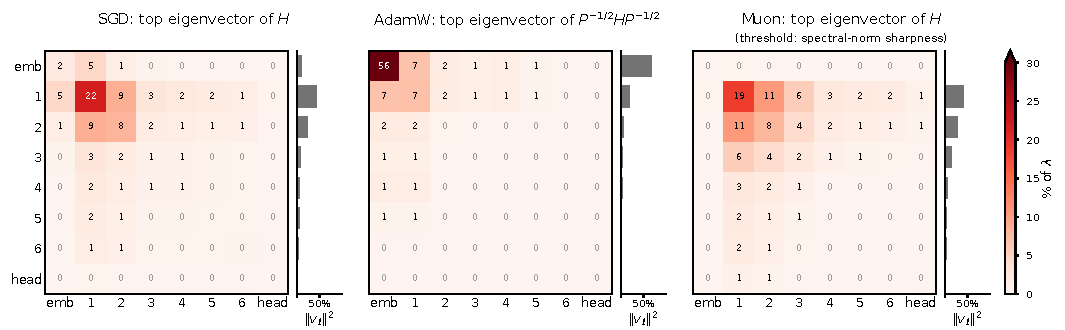
\includegraphics[page=1,width=\linewidth]{figures/ts10m/curvature.pdf}
\caption{Split of the top eigenvalue by layer\extra\ on TinyStories-10M at the edge of stability: cell $(\ell,m)$ is
$v_\ell^\top Av_m$ as a percentage of the eigenvalue, with $A$ the operator in each title (diagonal: curvature within
a layer; off-diagonal: between layers); bars: share of the direction $\|v_\ell\|^2$. Mean over data orders of each
run's mean over its saved checkpoints at the threshold (all saved steps for Muon). The AdamW panel uses 2 steps of
d0, because the preconditioned operator needs the optimizer state, which only the fork checkpoints keep.}
\label{fig:curv-layers}
\end{figure}

\begin{figure}[!htb]
\centering
\includegraphics[page=2,width=\linewidth]{figures/ts10m/curvature.pdf}
\caption{As \cref{fig:curv-layers}, with each block split into its attention and its MLP (each with the LayerNorm
that feeds it). Same steps; the AdamW panel again uses 2 steps of d0.}
\label{fig:curv-sublayers}
\end{figure}

\paragraph{Curvature between layers.\extra} On TinyStories-10M we recomputed the split of the eigenvalue over
pairs of layers at the saved checkpoints at the threshold (\cref{fig:curv-layers}). The sharp direction lies at
the input end: SGD's in blocks 1--2 (66\%), AdamW's, of $P^{-1/2}HP^{-1/2}$, in the embeddings (68\% at its two
steps at the threshold, both of d0; 66\% over all its saved steps), and Muon's, of $H$, which is not its
threshold operator, in blocks 1--3 (84\%). The share of the eigenvalue that comes from curvature between layers
is 66\% for SGD and 71\% for Muon; for AdamW it is 36\% overall, since most of its eigenvalue is the embeddings'
own curvature, and 62\% outside the embeddings. These shares are lower than the cross-block term $\chi$ above,
which also counts the curvature between the attention and MLP matrices of one layer. Split into sublayers
(\cref{fig:curv-sublayers}), SGD's direction lies mostly in the MLPs (52\%, against 37\% in attention; 28\% in
the first MLP), Muon's in attention (60\% against 37\%; 26\% in the first MLP, 23\% in the second attention and
16\% in the first), and AdamW's in the embeddings (68\%) and then the first attention (13\%). Between sublayers
comes 76\% of the eigenvalue for SGD, 80\% for Muon and 40\% for AdamW, and no cell is negative. The layer that
holds the direction keeps changing long after warmup (AdamW's between the embeddings and block 1 throughout
training, Muon's from block 1 to 2 after step 6000), so it does not mark a split.

\subsection{Break-even replication}
\label{sec:res-breakeven}

\begin{figure}[t]
\centering
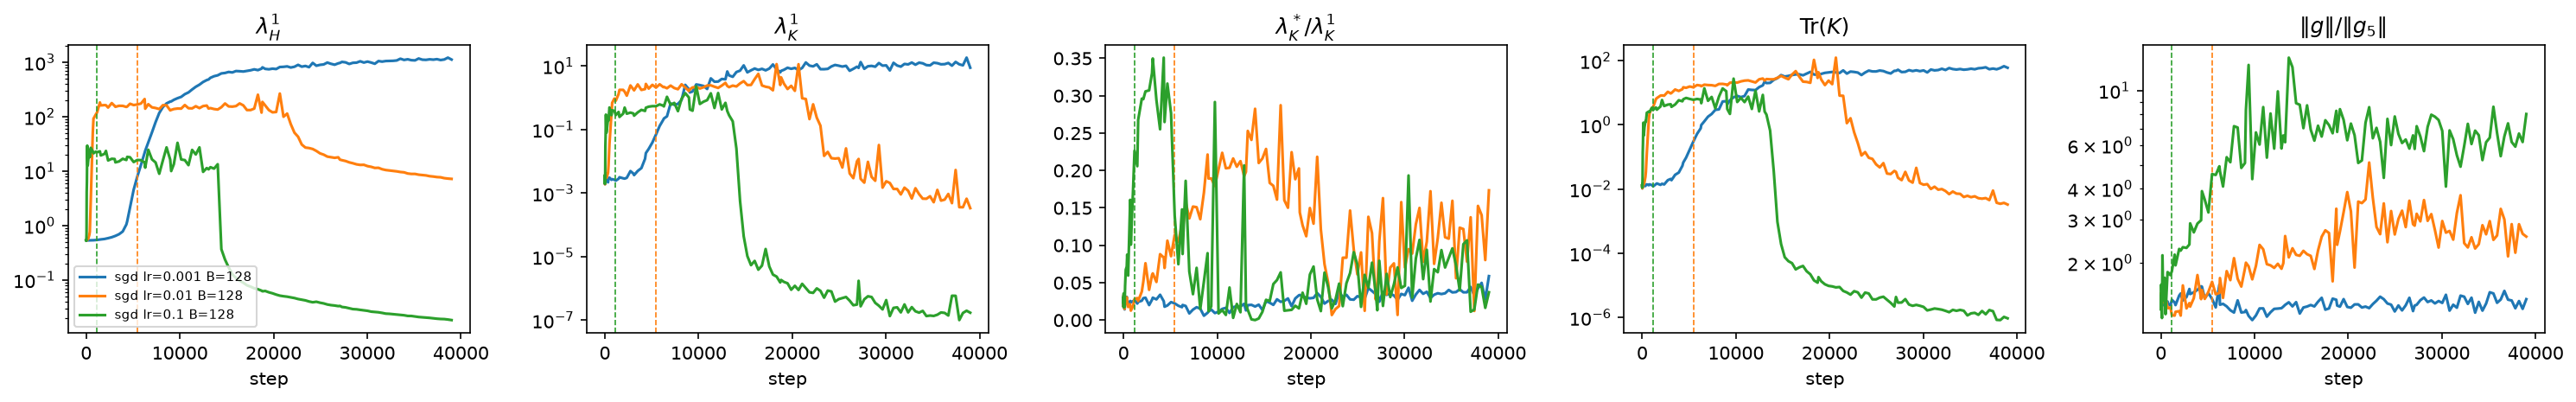
\includegraphics[width=\linewidth]{figures/breakeven/cifar/curves.png}\\[2pt]
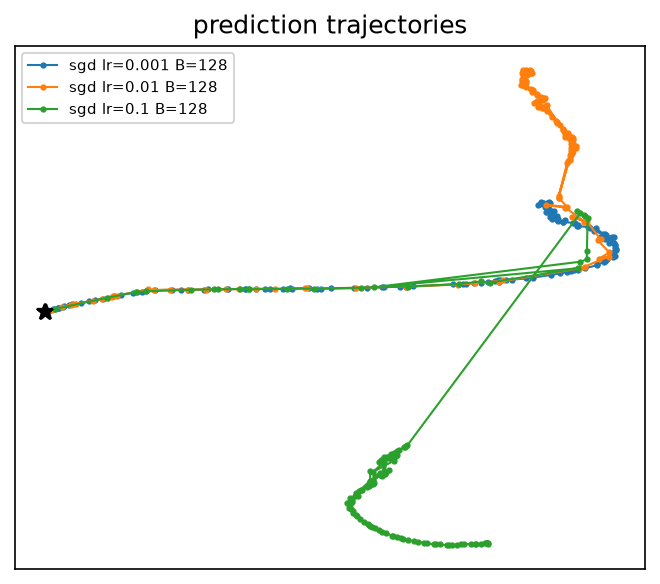
\includegraphics[width=0.27\linewidth]{figures/breakeven/cifar/trajectories.png}\hfill
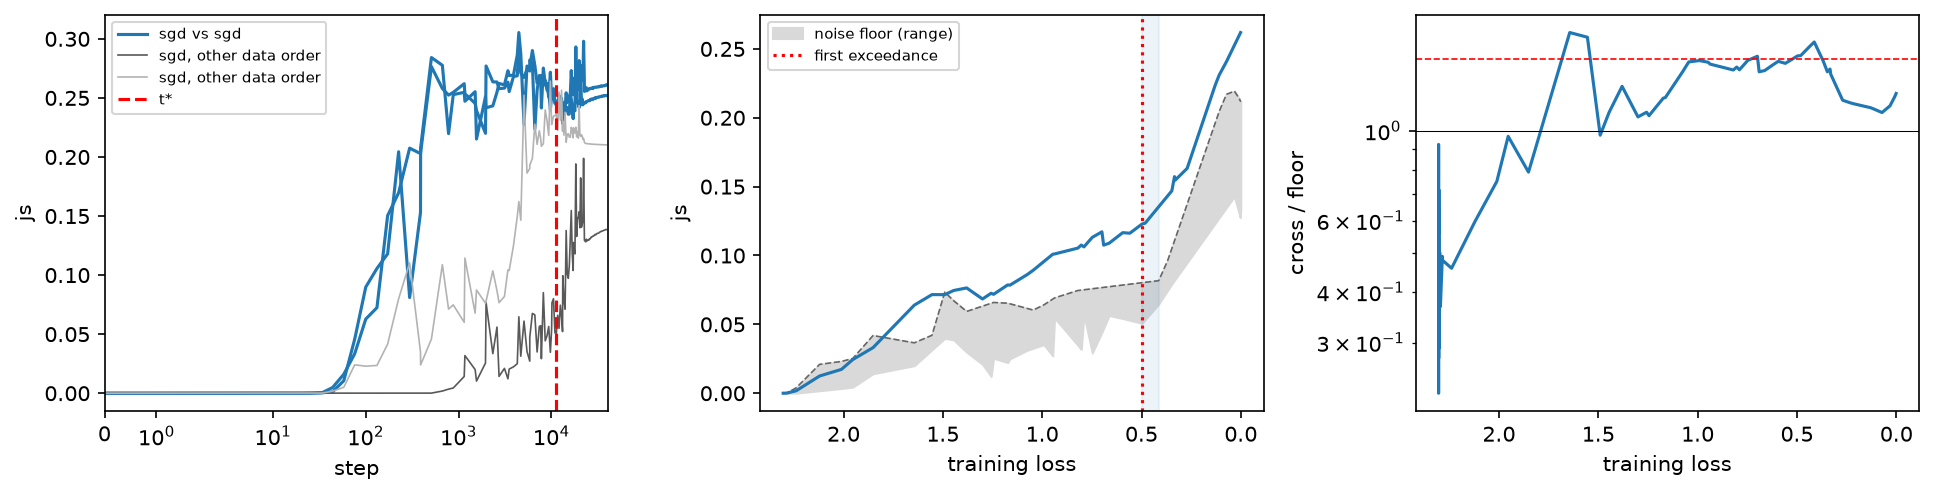
\includegraphics[width=0.71\linewidth]{figures/breakeven/cifar/figures/divergence_0.01_0.1.png}
%% python -m optsplit.analysis.breakeven --runs 'cifar_breakeven/sgd_lr*_d0'
\caption{The break-even analysis of \citet{jastrzebski2020breakeven} on CIFAR-10 with plain SGD at
$\eta\in\{0.001,0.01,0.1\}$, batch 128. Top: $\lambda_H^1$, $\lambda_K^1$, $\lambda_K^\ast/\lambda_K^1$,
$\operatorname{Tr}\hat K$ and $\|g\|/\|g_5\|$ against step ($d=0$). Bottom left: prediction trajectories
(PCA then UMAP), starting at the star. Bottom right: the divergence figure of \cref{fig:divergence} for
$\eta=0.01$ against $\eta=0.1$, with two data orders. Shakespeare in \cref{fig:app-breakeven}.}
\label{fig:breakeven}
\end{figure}

\paragraph{CIFAR-10.} The effects reported by \citet{jastrzebski2020breakeven} replicate
(\cref{fig:breakeven}). The larger the learning rate, the lower the sharpness in the early phase:
$\lambda_H^1$ levels off at about 1000, 200 and 20 for $\eta=0.001$, 0.01 and 0.1, that is at or below $2/\eta$,
and the maximum of $\lambda_K^1$ decreases with the learning rate in the same way. The larger rates also give a better-conditioned gradient covariance
(higher $\lambda_K^\ast/\lambda_K^1$) and a larger $\|g\|/\|g_5\|$. The relation between $\lambda_H^1$ and
$\lambda_K^1$ and $\Delta L$ is in \cref{fig:app-breakeven}. In prediction space the three runs share a path
from the initialization; $\eta=0.1$ leaves it first, then $\eta=0.01$. At equal steps the distance between
$\eta=0.01$ and $0.1$ is far above the data-order floor (bottom right, left panel). At equal training loss,
however, it is 1.0--1.75 times the floor at every loss below 1.8 (median 1.24); it exceeds 1.5 times the floor
at three consecutive levels only once (loss 0.50--0.41) and there is no persistent split. For $\eta=0.001$
against $0.01$ the ratio is 19 near the initialization, where the floor is near zero, and 0.57--2.08 below loss
1.5 (median 1.04), with four short episodes and no persistent split. As for the optimizers, most of the
separation in time is one run being faster.

\paragraph{Language models.\extra} On Shakespeare, plain SGD at 0.1 and 0.3 without warmup blows up in the first
ten or so steps, where the distance between any two runs, floor pairs included, approaches 1 bit; the runs
recover but reach only training loss 3.09 (the lowest common loss). At equal loss the distance between the two
rates is at most 1.17 times the floor and no split is found (\cref{tab:tstar}).
$\lambda_K^\ast/\lambda_K^1$ rises over training at both rates (\cref{fig:app-breakeven}), and $\lambda_H^1$ is lower at 0.3 apart from
spikes. At $\eta=0.03$ the runs do not blow up; against 0.1 the ratio exceeds the floor in one episode (loss
3.74--3.28, at most 5.2 times the floor, in 68\% of resamples) and is 0.90 at the lowest common loss, 3.13. On
TinyStories-10M the three rates reproduce the sharpness and noise effects: $\lambda_H^1$ levels off at about 125,
35 and 20 for $\eta=0.03$, 0.1 and 0.3, and $\lambda_K^1$ and $\operatorname{Tr}\hat K$ decrease with the
learning rate; but $\lambda_K^\ast/\lambda_K^1$ is, if anything, higher at the smallest rate, the opposite of
CIFAR-10. In prediction space 0.03 against 0.1 shows the pattern of the optimizer pairs: up to 151 times the
floor at loss 7.4, one episode down to loss 5.14, and 0.97 times the floor (median) below loss 4, down to the
lowest common loss 2.92 (\cref{fig:app-breakeven2}). The rate 0.3 recovers slowly from its initial blow-up, so
0.1 against 0.3 is compared only down to loss 4.80 (one episode, 7.78--6.24, ratio 1.07 at the end).

\paragraph{Batch size.\extra} On CIFAR-10 at $\eta=0.05$, batch 30 against 300 also replicates the sharpness effect
(the smaller batch levels off at a lower $\lambda_H^1$, about 12 against 50), and at equal loss the two batch
sizes are 0.66--2.14 times the floor below loss 2 (median 1.22; at most 3.1 near the initialization), with no
episode and no persistent split (\cref{fig:app-breakeven2}).

\subsection{Function metrics}
\label{sec:res-metrics}

\begin{figure}[t]
\centering
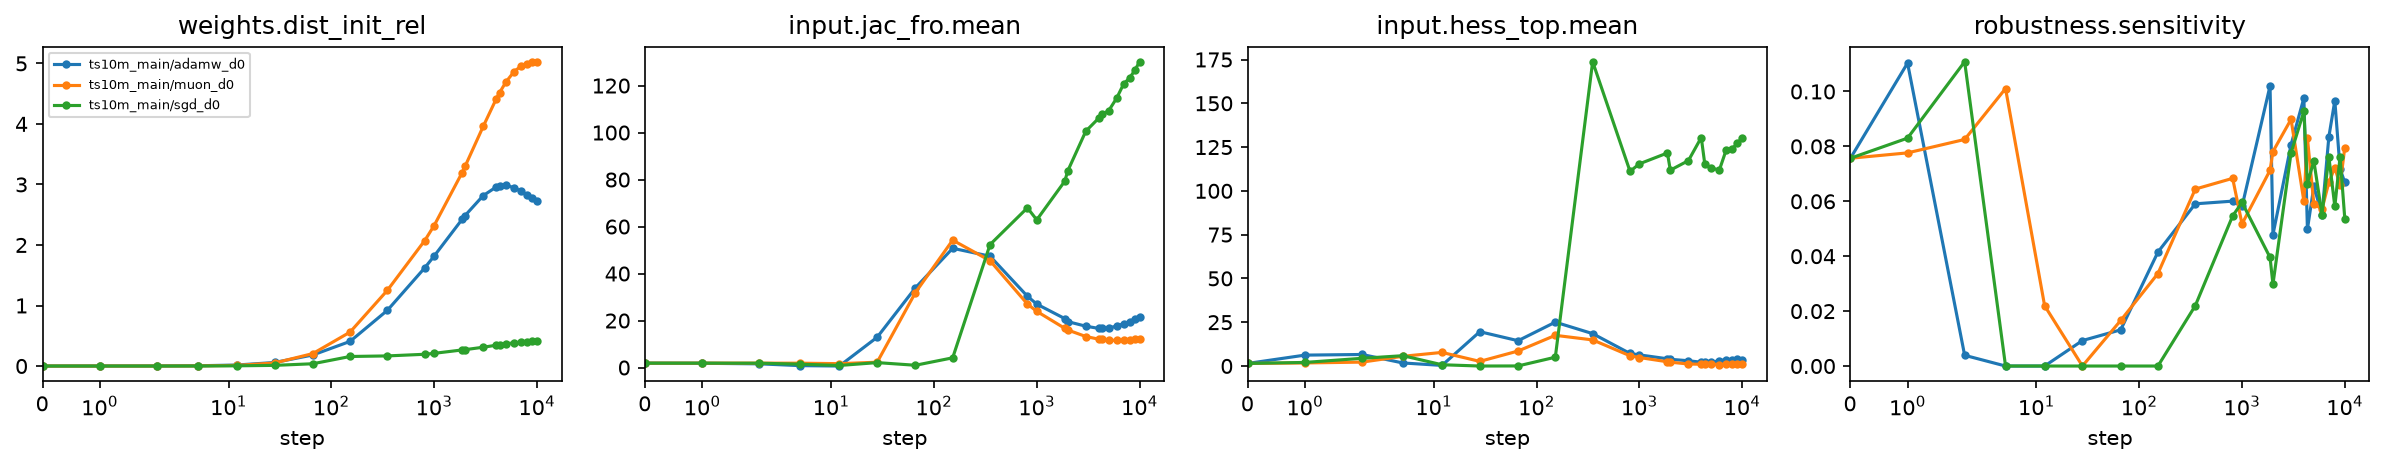
\includegraphics[width=\linewidth]{figures/ts10m/function_metrics.png}
%% python -m optsplit.metrics.run 'ts10m_main/*_d0' --steps all
%% python -m optsplit.analysis.plots function --runs 'ts10m_main/*_d0' --keys weights.dist_init_rel input.jac_fro.mean input.hess_top.mean robustness.sensitivity
\caption{Function metrics over training for the $d=0$ runs on TinyStories-10M: distance of the weights from the
initialization relative to the initial norm, Frobenius norm of the input Jacobian of the softmax output, top
eigenvalue of the input Hessian of the loss (inputs are the token embeddings), and one-token substitution
sensitivity (\cref{app:metrics}).}
\label{fig:metrics}
\end{figure}

\begin{table}[t]
\centering\small
\caption{Final function metrics on TinyStories, mean over the five data orders (standard deviations are small
except for SGD's spectral norms and stable rank). ``Hidden'' are the matrices in the transformer blocks, the ones
Muon updates; the stable rank is $\|W\|_F^2/\|W\|_2^2$.}
\label{tab:metrics}
\begin{tabular}{@{}lrrrrrr@{}}
\toprule
 & \multicolumn{3}{c}{TinyStories-10M} & \multicolumn{3}{c}{TinyStories-30M} \\
\cmidrule(lr){2-4}\cmidrule(l){5-7}
 & SGD & AdamW & Muon & SGD & AdamW & Muon \\
\midrule
$\|\theta\|_2$ & 105 & 265 & 485 & 156 & 369 & 857 \\
$\|\theta\|_\infty$ & 4.37 & 2.09 & 1.85 & 3.33 & 2.58 & 2.28 \\
$\max\|W\|_2$ (hidden) & 3.5 & 12.4 & 14.1 & 7.6 & 15.0 & 22.9 \\
$\|\theta\|_\infty/\|\theta\|_2$ ($\times10^{3}$) & 41.6 & 7.9 & 3.8 & 21.3 & 7.0 & 2.7 \\
stable rank (hidden, mean) & 56 & 41 & 75 & 56 & 47 & 90 \\
$\|\theta-\theta_0\|/\|\theta_0\|$ & 0.40 & 2.72 & 5.04 & 0.61 & 2.83 & 6.56 \\
input Jacobian (Frobenius) & 131.7 & 21.6 & 12.5 & 72.7 & 15.2 & 7.8 \\
input Hessian $\lambda_{\max}$ & 123.6 & 3.5 & 1.1 & 37.2 & 2.4 & 0.5 \\
substitution sensitivity & 0.070 & 0.082 & 0.067 & 0.076 & 0.060 & 0.075 \\
top-1 accuracy & 0.576 & 0.651 & 0.657 & 0.637 & 0.677 & 0.680 \\
\bottomrule
\end{tabular}
\end{table}

The raw norms mostly measure how far each optimizer moves the weights (\cref{tab:metrics}): Muon ends 5.0--6.6
initial norms away from the initialization, AdamW 2.7--2.8 and SGD 0.4--0.6, and $\|\theta\|_2$ and the largest
spectral norm of the hidden matrices follow the same order. So SGD having the smallest $\ell_2$ norm, and Muon the
largest spectral norm, says little about implicit bias. The scale-free versions\extra\ match the predicted geometries
in part. The ratio $\|\theta\|_\infty/\|\theta\|_2$, small when the entries are even, is 3--5 times smaller for
AdamW than for SGD, as Adam's $\ell_\infty$ bias predicts \citep{zhang2024adam}; and the mean stable rank of the
hidden matrices, large when their singular values are even, is highest for Muon (75 and 90 against 41--56), as
its spectral bias predicts \citep{fan2025spectral}. Muon also has the smallest $\|\theta\|_\infty/\|\theta\|_2$.
The weights therefore carry the geometry of their optimizer while the functions of AdamW and Muon are within the
data-order floor of each other (\cref{sec:res-route}), in line with the barriers of \cref{sec:res-swap}.

In input space SGD's function looks much sharper: its input Jacobian is 5--11 times and its top input-Hessian
eigenvalue 15--110 times those of AdamW and Muon. The inputs are the token embeddings, which SGD moves least
(Frobenius norm of the embedding matrix 27 for SGD against 97 for AdamW and 175 for Muon on TinyStories-10M), and
the pre-LayerNorm transformer normalizes the residual stream, so derivatives with respect to the embeddings shrink
as the embeddings grow; much of the difference is therefore one of scale. One-token substitution sensitivity,
which does not depend on that scale, is 0.06--0.08 for all three; and the input Jacobian times the embedding
norm is about the same for AdamW and Muon ($2.1$ and $2.2\times10^3$) and 1.7 times higher for SGD. Over training
(\cref{fig:metrics}) the input Jacobian of AdamW and Muon peaks at about step 200, the end of warmup, and then
falls, while SGD's keeps rising.

On Shakespeare (\cref{tab:app-metrics-shk}) AdamW's learning rate of $3\times10^{-4}$ moves the weights by only
0.25 initial norms, as little as SGD (0.36), and the two have the same $\|\theta\|_\infty/\|\theta\|_2$
($12.4$ and $12.3\times10^{-3}$): the $\ell_\infty$ geometry only shows once the weights leave the
initialization. Muon again has the largest stable rank (99 against 48 and 63), and, as it memorizes, twice to
four times the substitution sensitivity of the others (0.19 against 0.10 and 0.05).

\paragraph{Representations\extra.} Between weights and outputs sit the hidden states (\cref{fig:cka}). On
TinyStories, AdamW and Muon trained on the same data have less similar representations than two data orders of
either optimizer, but not by much outside the first block: linear CKA 0.69 and 0.66 after the first block
against 0.87--1.0, and 0.78--0.97 against 0.85--0.98 after the others, 0.82--0.85 against 0.85--0.88 after the
final LayerNorm. SGD's representations are not even reproducible across its own data orders (0.57--0.83), and
pairs with SGD are lower still. On Shakespeare, where Muon memorizes, AdamW and Muon differ clearly (0.40--0.87).
Another initialization moves the representations as much as another data order. So the optimizer's mark fades
from the weights (their geometry, and barriers in the middle blocks) through the representations (a small CKA gap) to the
outputs (none).

\begin{figure}[t]
\centering
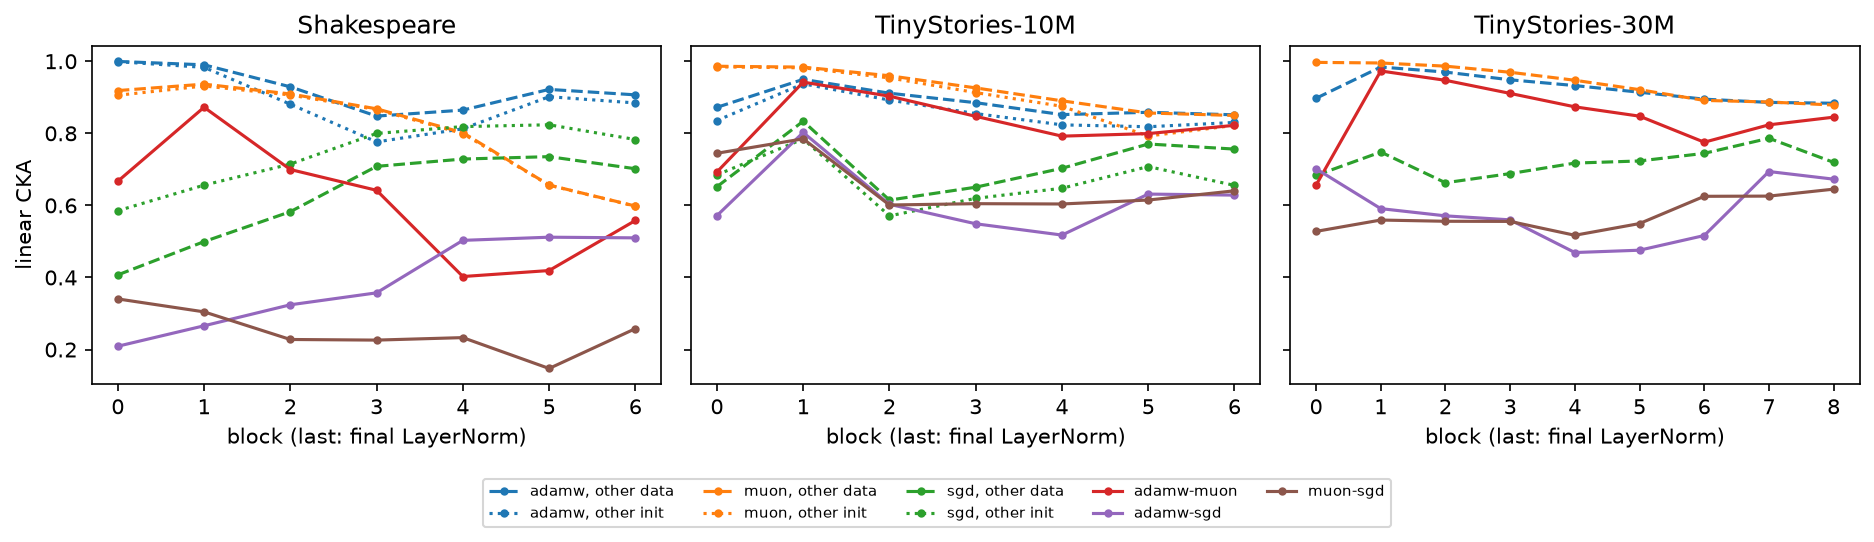
\includegraphics[width=\linewidth]{figures/cka.png}
%% python -m optsplit.analysis.cka 'S_main/*' 'S_initseed/*' --out analysis/S
\caption{Linear CKA\extra\ between the final hidden states of two pure runs after each transformer block (the last
point is the final LayerNorm), averaged over pairs. Solid: other optimizer, same initialization and data order;
dashed: same optimizer, other data order; dotted: same optimizer, other initialization (not run on
TinyStories-30M).}
\label{fig:cka}
\end{figure}

\paragraph{Off the data distribution\extra.} The optimizers could agree on the data and differ elsewhere, where
the data do not constrain the function and an implicit bias has room to act. We compared the final functions of
the pure runs on the 32 validation sequences, on the same sequences with their tokens shuffled within each
sequence, and on uniformly random tokens (\cref{fig:ood}). Off the distribution every pair of runs differs much
more (on TinyStories, 0.20--0.25 bits on shuffled and 0.30--0.40 on random tokens, against 0.05--0.06 on
validation), but the optimizer adds no more than the data order does: AdamW and Muon are 0.90--1.07 floors
apart on every input type in all three settings. SGD, less trained at equal steps, is 1.2--2.7 floors from the
adaptive optimizers on validation but only 1.05--1.8 off the distribution, so what separates it is how well it
fits the data, not how it extrapolates.

\begin{figure}[t]
\centering
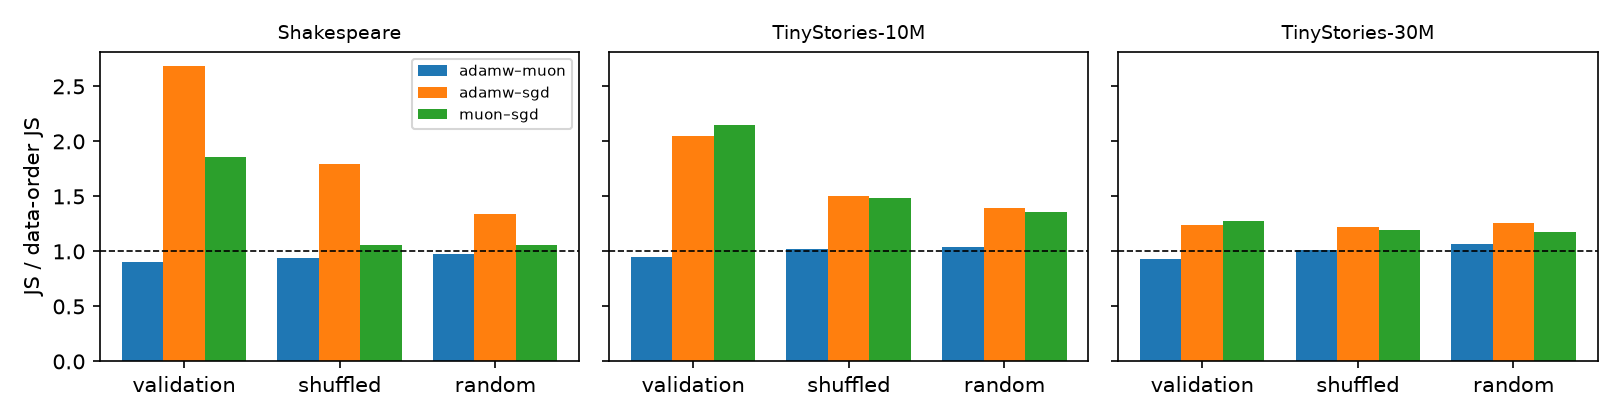
\includegraphics[width=\linewidth]{figures/ood.png}
%% python -m optsplit.analysis.ood 'S_main/*' 'S_initseed/*' --out analysis/S
\caption{Distance $D_\JS$ off the data distribution\extra\ between the final functions of two optimizers (same
initialization and data order), averaged over the five data orders, over the larger of the two optimizers' mean distance between data orders, on
validation sequences, on the same sequences with shuffled tokens, and on uniformly random tokens.}
\label{fig:ood}
\end{figure}

\paragraph{Metrics under swaps.} \Cref{fig:swap-metrics} places each fork's final metrics (the scale-free ones
added after the plan\extra) between those of pure A (0) and pure B (1). The weight metrics follow whichever optimizer moved the weights more, not the one that
decides the function. Forks into SGD keep the old optimizer's $\|\theta\|_\infty/\|\theta\|_2$ and input
Jacobian after switching at step 400 or later (shift $\le0.37$), although at steps 400--1000 their function is
within 1.0--1.4 floors of pure SGD (\cref{fig:swap}); Muon to SGD keeps Muon's stable rank at every fork step.
Forks from SGD take the new optimizer's metrics, as they take its function. Between AdamW and Muon, whose
functions cannot be told apart, the late forks are mixtures: switching at step 4000 goes only 0.28 (AdamW to
Muon) and 0.45 (Muon to AdamW) of the way to the new optimizer's stable rank, and 0.4--0.6 of the way in
$\|\theta\|_\infty/\|\theta\|_2$. The geometry of the endpoint records both optimizers and their order,
while the function records only the faster of the two. On Shakespeare
the same holds where the pure gap exceeds the noise, with Muon, which moves the weights furthest, setting the
geometry (\cref{fig:app-swap-metrics}). On TinyStories-30M the picture is the same, from a later fork step for
the swaps into SGD: switching at step 800 or later keeps the old optimizer's $\|\theta\|_\infty/\|\theta\|_2$
(shift $\le0.20$), and at step 1400 or later its input Jacobian ($\le0.19$), while up to step 3000 the function
of these forks is within 1.02--1.21 floors of pure SGD; AdamW and Muon swapped at step 8000 go 0.29 and 0.65 of
the way in stable rank and 0.45 in $\|\theta\|_\infty/\|\theta\|_2$.

\begin{figure}[t]
\centering
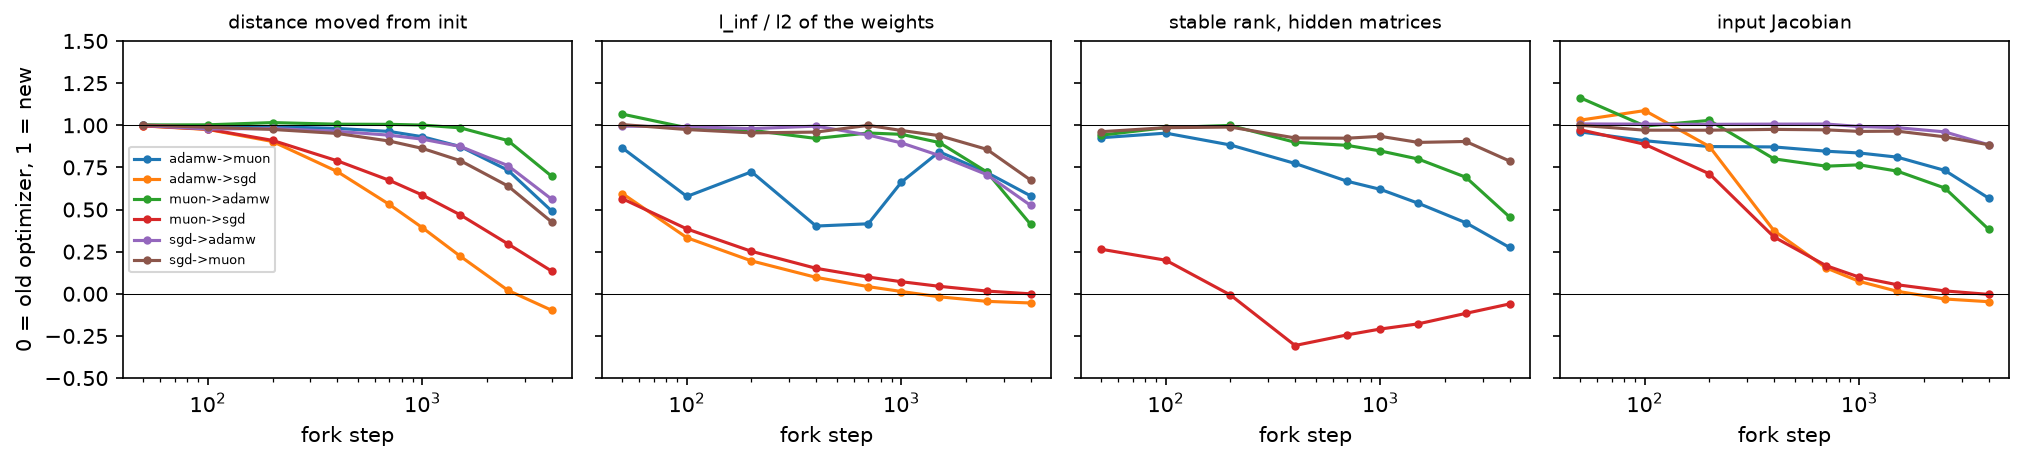
\includegraphics[width=\linewidth]{figures/ts10m/swap_metrics.png}
%% python -m optsplit.analysis.swap --forks 'ts10m_forks/*' --pure 'ts10m_main/*' --out analysis/ts10m/swap
%% python -m optsplit.analysis.plots swap --swap-json analysis/ts10m/swap.json --out analysis/ts10m/figures
\caption{Final metrics of the forks on TinyStories-10M as a fraction of the gap between pure A (0) and pure B
(1), against the fork step. Pairs whose pure gap is under three data-order standard deviations are left out
(AdamW--SGD in stable rank).}
\label{fig:swap-metrics}
\end{figure}

\subsection{Further controls\extra}
\label{sec:res-controls}

\begin{figure}[t]
\centering
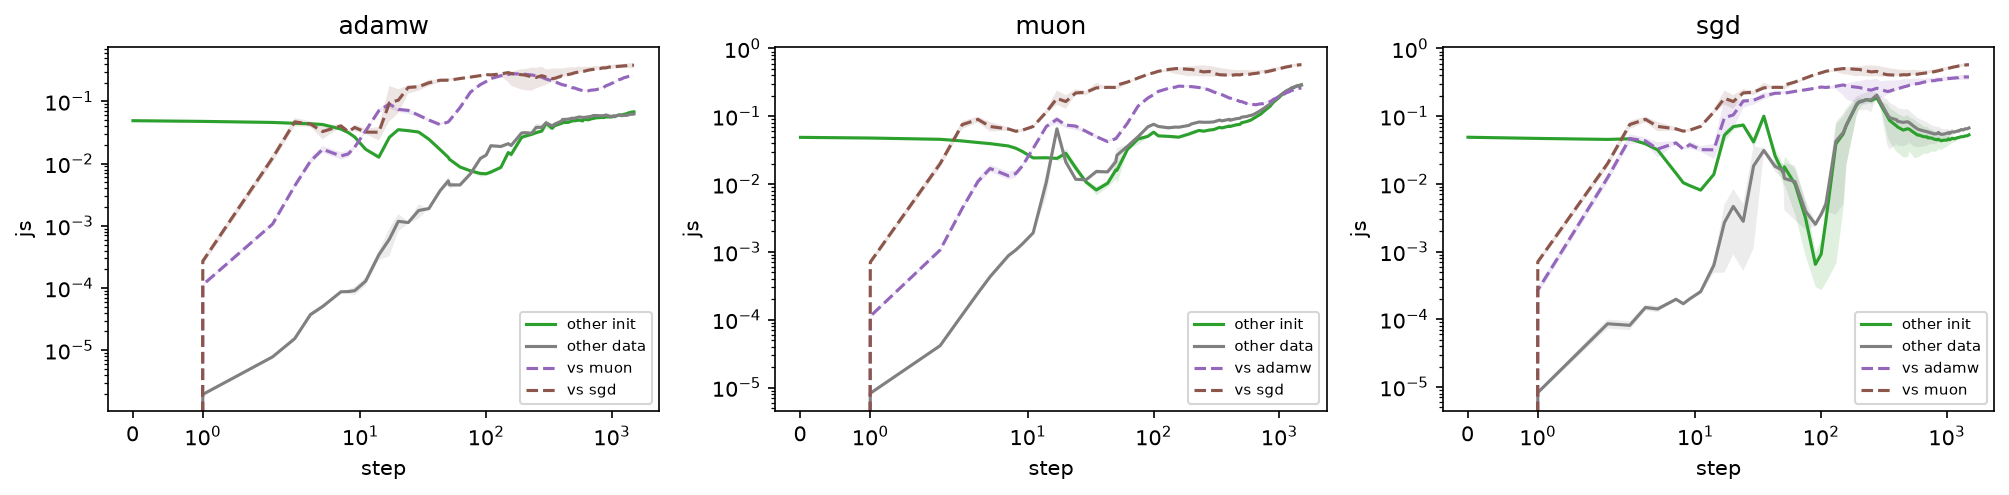
\includegraphics[width=\linewidth]{figures/shakespeare/initseed_js.png}\\[2pt]
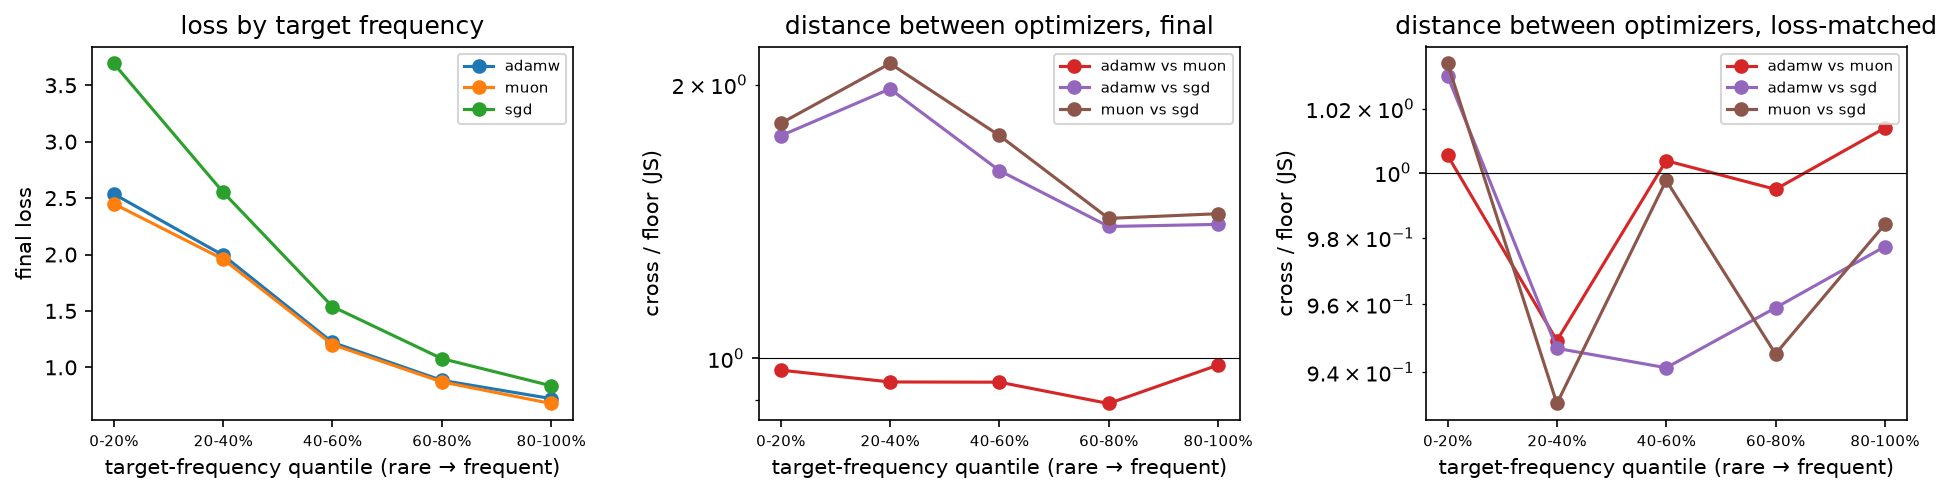
\includegraphics[width=\linewidth]{figures/ts10m/tokens.png}\\[2pt]
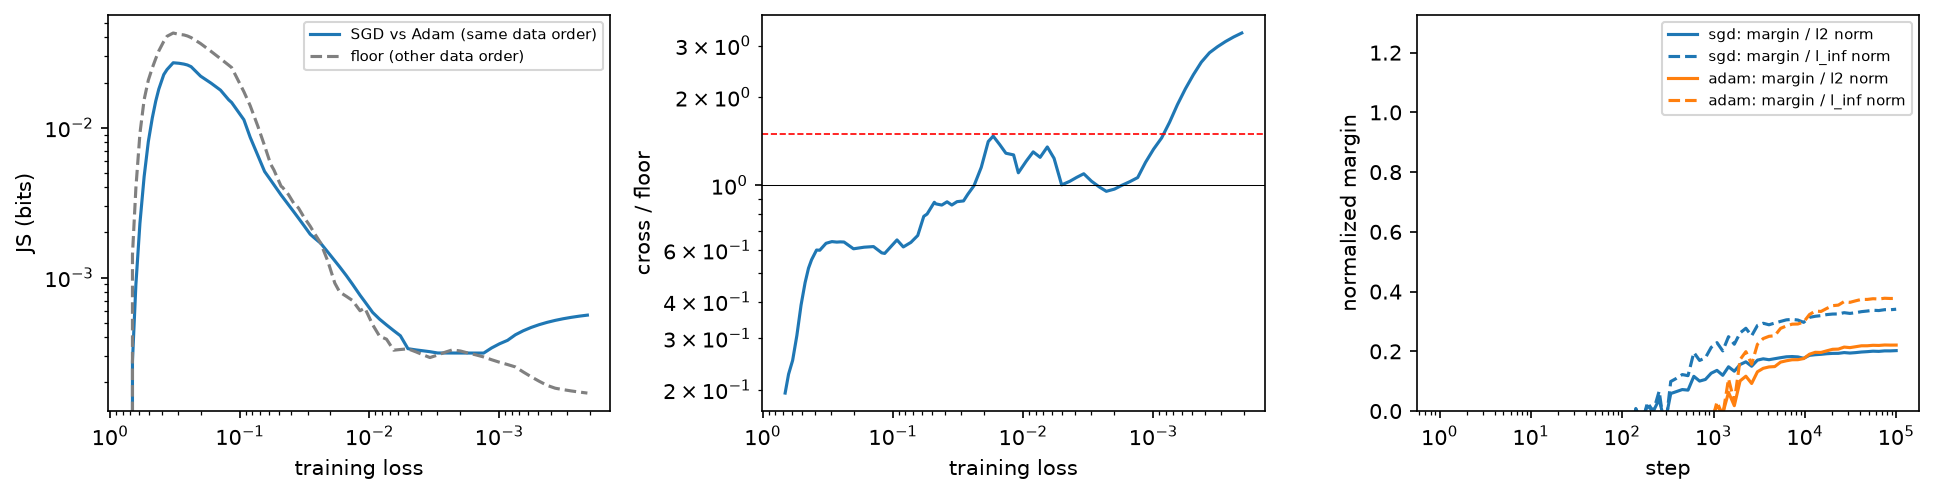
\includegraphics[width=\linewidth]{figures/linear/linear_control.png}
%% python -m optsplit.analysis.initseed 'shakespeare_main/*' 'shakespeare_initseed/*' --out analysis/shakespeare
%% python -m optsplit.analysis.tokens 'ts10m_main/*' --out analysis/ts10m
%% python scripts/linear_control.py --out analysis/linear
\caption{Controls added after the plan. Top: second initialization on Shakespeare; for each optimizer, at equal
steps, the distance to the same optimizer from the other initialization (same data order), to the same
optimizer with the other data order (same initialization), and to the other optimizers (same initialization
and data order); median and range over the pairs. Middle: TinyStories-10M by target-token frequency (quintiles
of the training frequency of the target, rare to frequent): final validation loss of each optimizer (mean over
data orders), and the distance between optimizers over the floor at the final step and at the lowest training
loss both runs reach. Bottom: the linear positive control; loss-matched JS distance between SGD and Adam on the
test points against the data-order floor (left), their ratio with the margin $1+m_\times=1.5$ (middle), and the
$\ell_2$- and $\ell_\infty$-normalized margins over training (right).}
\label{fig:controls}
\end{figure}

\paragraph{Second initialization.} All other runs share one initialization, so the floor varies only the data
order. We repeated the main runs of Shakespeare and TinyStories-10M from a second initialization (seed 1) with
data orders 0 and 1, without curvature measurements. On Shakespeare (\cref{fig:controls}, top) the distance
between the two initializations starts at 0.05 bits, falls to about 0.01 by step 10--100 and from about step 100
on equals the data-order floor for every optimizer; at the final step it is 0.068 against 0.063 (AdamW), 0.288
against 0.292 (Muon) and 0.053 against 0.067 (SGD). The split analysis at the second initialization, with two
data orders, reproduces that at the first: AdamW--Muon has episodes at loss 4.18--2.86 and 2.41--2.02 (first
initialization: 4.23--2.77 and 2.30--2.12) and no persistent split; AdamW--SGD 4.18--3.04 and 2.77--2.54 (first:
4.23--3.10), no persistent split; and Muon--SGD again has a persistent split, from loss 2.80 (first: 2.82).
On TinyStories-10M (\cref{fig:app-initseed}) the two distances also agree from about step 100 on, and at the
final step the initialization, the data order and the change between AdamW and Muon all give the same distance:
0.054, 0.062 and 0.058 bits from AdamW, 0.055, 0.059 and 0.058 from Muon. The episodes are again close to those
of the first initialization, AdamW--Muon 8.31--4.27 (first: 8.26--4.85), AdamW--SGD 8.31--6.21 (8.26--6.32) and
Muon--SGD 8.43--6.78 (8.38--5.81), with no persistent split. Changing the initialization thus moves the function by as much as changing the data
order, and the structure of the episodes does not depend on the initialization.

\paragraph{Rare and frequent tokens.} \citet{kunstner2024heavytail} attribute Adam's advantage over SGD on
language models to the rare classes of a heavy-tailed vocabulary. We grouped the probe positions by the training
frequency of their target token (\cref{fig:controls}, middle, for TinyStories-10M). SGD's loss gap is concentrated on the rare tokens:
on TinyStories-10M it is 1.15 nats above AdamW on the rarest fifth and 0.12 on the most frequent (TinyStories-30M:
0.48 and 0.07). At the final step its distance from AdamW and Muon is also largest on the rare tokens (1.8--2.1
times the floor, against 1.4 on the most frequent), but at the lowest training loss both runs reach it is
0.93--1.03 times the floor in every bin, for every pair on TinyStories. The gap on rare tokens is a difference in
speed, not in the function learned at equal loss.

\paragraph{A positive control.} Since the detector finds no persistent split between AdamW and Muon, we checked
that it finds one where theory predicts it. Logistic regression on linearly separable data ($d=50$, $n=200$,
labels from a sparse teacher on 3 coordinates, 2000 test points), from zero initialization with batch 20, trained
by SGD with momentum ($\eta=0.1$) and by Adam ($\eta=0.01$) for $10^5$ steps with five data orders: in the limit
gradient descent converges in direction to the $\ell_2$ max-margin classifier \citep{soudry2018separable} and Adam
to the $\ell_\infty$ one \citep{zhang2024adam}. The same loss-matched JS rule, on the test predictions, finds the
ratio below 1.5 down to training loss $10^{-2}$ (at most 1.47) and a persistent split from loss
$7.5\cdot10^{-4}$, with the ratio up to 3.3 (\cref{fig:controls}, bottom). The detector can see a split, and in
the linear case the split appears near interpolation, far below the losses our language models reach. Neither
optimizer is at its limit after $10^5$ steps: Adam's normalized margins exceed SGD's in both norms (0.221 against
0.202 in $\ell_2$, 0.377 against 0.341 in $\ell_\infty$).

\paragraph{Training into memorization.} If the language models split only near interpolation, as the linear model
does, our runs may simply stop too early. On Shakespeare we therefore trained AdamW and Muon for 8000 steps instead
of 1500 (same learning rates, cosine schedule over the longer run, five data orders each), so that both memorize:
AdamW's training loss falls to 0.09 and its validation loss rises to 4.6. The loss-matched ratio
(\cref{fig:app-long}; \cref{fig:overview}, top left, red) has a single early episode (loss 4.23--2.64) and then falls
steadily to 1.0 at the lowest common loss, 0.09; with top-1 disagreement the picture is the same (episode
4.23--2.85, no persistent split). At the final step the two optimizers on the same data order are as far apart as
two data orders of either (0.359 bits against floors of 0.355 and 0.324). Memorizing the training set, AdamW and
Muon reach functions that differ on held-out text by a lot, but by no more than two data orders do.

\paragraph{Other learning rates.} The comparisons above use one tuned learning rate per optimizer. The sweep
runs (data order 0, same initialization) give the comparison at every other rate for free: each against the
tuned run of every optimizer on the same data, at equal training loss, over the data-order floor of the tuned
runs, summarized by the median below the bigram loss (\cref{fig:lr-robust}). On TinyStories every rate that
trains stably, a 27-fold range for AdamW, 8-fold for Muon and 3- to 10-fold for SGD, is within 0.80--1.11 floors
of all three tuned optimizers, with one exception: SGD at 0.1 is 1.35 floors from tuned SGD at 0.03 on
TinyStories-10M, further than from tuned AdamW or Muon. Only rates at the edge of stability (Muon at 0.08, SGD
at 0.3 on TinyStories-10M) are 1.5--2.3 floors away, and higher ones diverge. On Shakespeare, where SGD does not get below the bigram loss
at most rates, AdamW at 3--13 times its tuned rate is 1.5--1.6 floors from tuned AdamW but 1.03--1.06 from tuned
Muon, since the floor of a cross comparison is the larger of the two optimizers' floors and Muon's is large
(it memorizes). The floor of the tuned runs may not be the
floor at other rates, so this is a check, not a second analysis; but it shows that the absence of a split on
TinyStories is not a property of the chosen rates.

\begin{figure}[t]
\centering
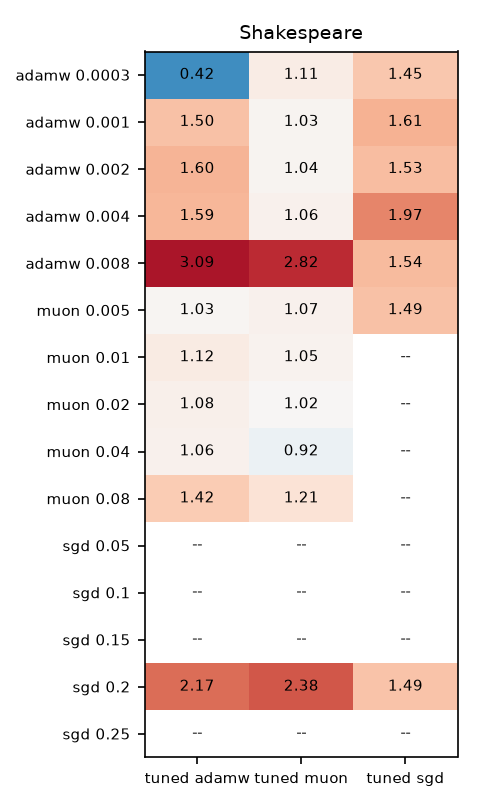
\includegraphics[width=0.32\linewidth]{figures/shakespeare/lr_robust.png}\hfill
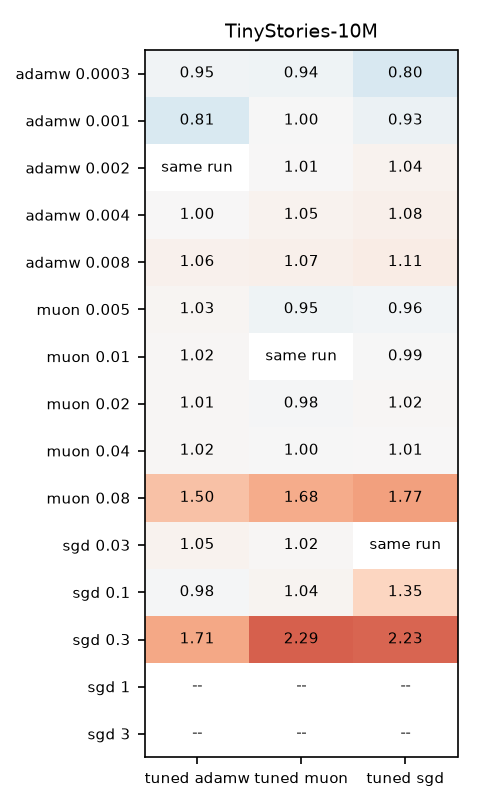
\includegraphics[width=0.32\linewidth]{figures/ts10m/lr_robust.png}\hfill
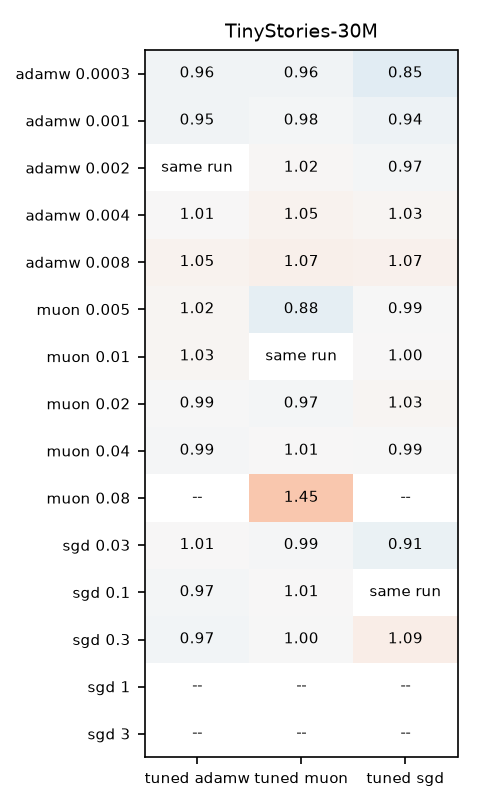
\includegraphics[width=0.32\linewidth]{figures/ts30m/lr_robust.png}
%% python -m optsplit.analysis.lr_robust --sweep 'S_lrsweep/*' --main 'S_main/*' --below 3.8 --out analysis/S
\caption{Each learning-rate sweep run (rows) against the tuned run of each optimizer (columns) on the same data
order: median loss-matched JS over the data-order floor of the tuned runs, below the bigram loss (2.47 on
Shakespeare, 3.8 on TinyStories). Blue below 1, red above; ``--'': diverged or never below that loss.}
\label{fig:lr-robust}
\end{figure}

\paragraph{Rates around the tuned one.} On TinyStories-10M we also trained each optimizer at $\tfrac14$,
$\tfrac12$, 2 and 4 times its tuned rate (SGD 0.0075--0.12, AdamW $5\cdot10^{-4}$--$8\cdot10^{-3}$, Muon
0.0025--0.04; data order 0, the schedule and length of the main runs) and compared each run with the run at the
tuned rate. At equal loss every rate stays within 0.8--1.1 times the data-order floor of the tuned runs, from
loss about 3--4 to the end, for all three optimizers. In a densMAP of the trajectories, one per optimizer
(\cref{fig:traj-lr}), the SGD runs at different rates take separate paths from about loss 3, while the AdamW runs
share one path down to loss 3, and so do the Muon runs. The embedding keeps neighbourhoods, not distances: in the
actual distances at equal loss the SGD rates do not split either.

\begin{figure}[t]
\centering
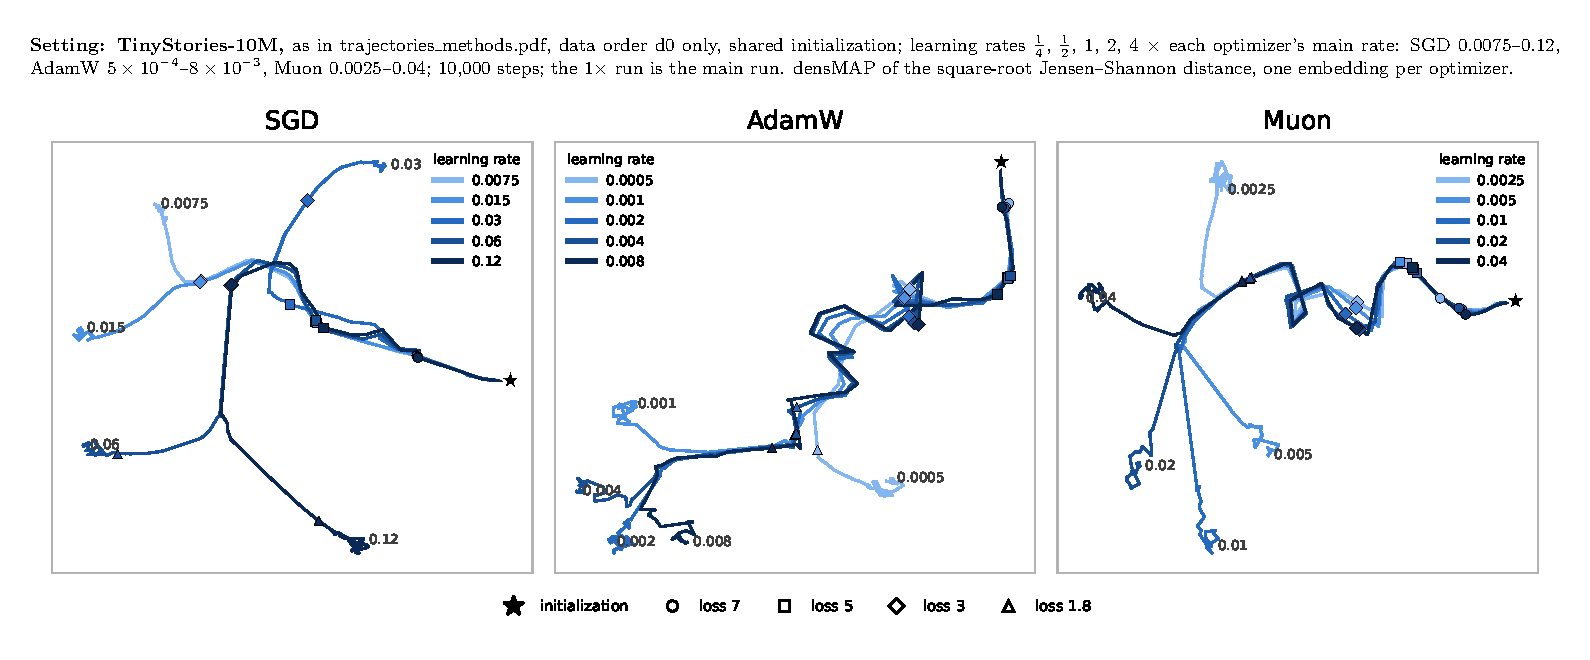
\includegraphics[page=1,width=\linewidth,trim=0 0 0 45,clip]{figures/ts10m/trajectories_lr.pdf}
\caption{Runs at $\tfrac14$ to 4 times each optimizer's rate on TinyStories-10M (data order 0, shared
initialization; the $1\times$ run is the main run): densMAP of the $\sqrt{\JS}$ distance between their logged
steps, one embedding per optimizer. Markers: the initialization and the steps at which each run reaches training
loss 7, 5, 3 and 1.8. densMAP keeps neighbourhoods, not distances.}
\label{fig:traj-lr}
\end{figure}

\FloatBarrier
%% =================================================================
\section{A model of the results\extra}
\label{sec:theory}
%% =================================================================

The results share one pattern: the optimizers differ in how they get somewhere (speed, route, weights,
curvature), but after warmup not in which function they compute at a given training loss. Here we
give a simple model of this pattern and of the role of the break-even point, with proofs or derivations, a toy
model in which every quantity is exact (\cref{fig:toy}), and checks against the measurements.

\paragraph{Setup.} Contexts $c\sim\cD$ have next tokens $y\sim q(\cdot\mid c)$, and a predictor $\pi$ has loss
$L(\pi)=\mathbb E_c\,\mathbb E_{y\sim q(\cdot\mid c)}[-\log\pi(y\mid c)]$. For a statistic $s$ of the context
(nothing, the last token, the last $k$ tokens), let $\mathcal F_s$ be the predictors that depend on $c$ only
through $s(c)$: the unigram, bigram, \dots\ predictors. $\mathcal F_s$ is convex; its best element is the n-gram
model of the data, $q_s(\cdot\mid s)=\mathbb E[q(\cdot\mid c)\mid s(c)=s]$, with loss the n-gram entropy $H_s$,
and by the tower property every $\pi\in\mathcal F_s$ satisfies
\begin{equation}
L(\pi)=H_s+\mathbb E_s\,\KL\big(q_s(\cdot\mid s)\,\|\,\pi(\cdot\mid s)\big).
\label{eq:pythagoras}
\end{equation}

\paragraph{Proposition 1 (funnel).} \emph{If $\pi_A,\pi_B\in\mathcal F_s$ have excess losses $\Delta
L_A=L(\pi_A)-H_s$ and $\Delta L_B$ (in nats), then, with $\JS$ in bits,}
\begin{equation}
\mathbb E_s\JS(\pi_A,\pi_B)\le\sqrt2\big(\sqrt{\Delta L_A}+\sqrt{\Delta L_B}\big),\qquad\text{and}\qquad
\mathbb E_s\JS(\pi_A,\pi_B)\le\frac{\Delta L_A+\Delta L_B}{2\ln2}\,(1+o(1))\ \text{ as }\Delta L_A,\Delta L_B\to0.
\label{eq:funnel}
\end{equation}
\emph{Proof.} $\sqrt{\JS}$ is a metric \citep{endres2003metric}. For one outcome with probabilities $p,q$ the
divergence (in nats) is $\frac{p+q}{2}(\ln2-h(t))$ with $t=p/(p+q)$ and $h$ the binary entropy, and $\ln2-h(t)\le
\ln2\,|2t-1|$ because the left side is convex and the two agree at $t\in\{0,\frac12,1\}$; summing, $\JS$ in bits
is at most the total variation $\mathrm{TV}$. With Pinsker's inequality $\mathrm{TV}\le\sqrt{\KL/2}$,
$\JS(\pi_A,\pi_B)\le(\sqrt{\JS(\pi_A,q_s)}+\sqrt{\JS(q_s,\pi_B)})^2\le2\,\mathrm{TV}(\pi_A,q_s)+2\,\mathrm{TV}(q_s,\pi_B)
\le\sqrt2(\sqrt{\KL(q_s\|\pi_A)}+\sqrt{\KL(q_s\|\pi_B)})$; take the mean over $s$, use Jensen's inequality and
\eqref{eq:pythagoras}. For the second bound, $\JS(q,\pi)$ in nats and $\KL(q\|\pi)$ are $\frac18$ and
$\frac12$ of $\sum_y(\pi(y)-q(y))^2/q(y)$ to leading order, and $(a+b)^2\le2a^2+2b^2$. $\square$

Within a class, all predictors with a given loss thus lie in a shell around $q_s$ that shrinks with the excess
loss, whichever optimizer produced them. Two optimizers can be far apart at equal loss only when the loss is far
above the optimum of the class their functions lie in, or when the class has no best element: on separable data
the loss tends to zero along directions chosen by each optimizer's implicit bias
\citep{soudry2018separable,zhang2024adam}, which is where the linear control splits (\cref{sec:res-controls}).
Networks learn the statistics of their data roughly in order of complexity \citep{belrose2024statistics}, and ours
pass close to the bottom of the bigram funnel: on Shakespeare all three optimizers come within 0.036--0.041 bits
of $q_2$ at losses 2.46--2.48, 0.01--0.03 nats above the bigram entropy of the training split ($H_2=2.452$), where
the AdamW--Muon ratio is 0.91 (\cref{sec:res-route}). In the toy below, where the model can only represent
bigram predictors, \eqref{eq:funnel} holds exactly, and the loss-matched distance between optimizers falls with
the excess loss as the second bound allows (\cref{fig:toy}, bottom left).

\begin{figure}[!htb]
\centering
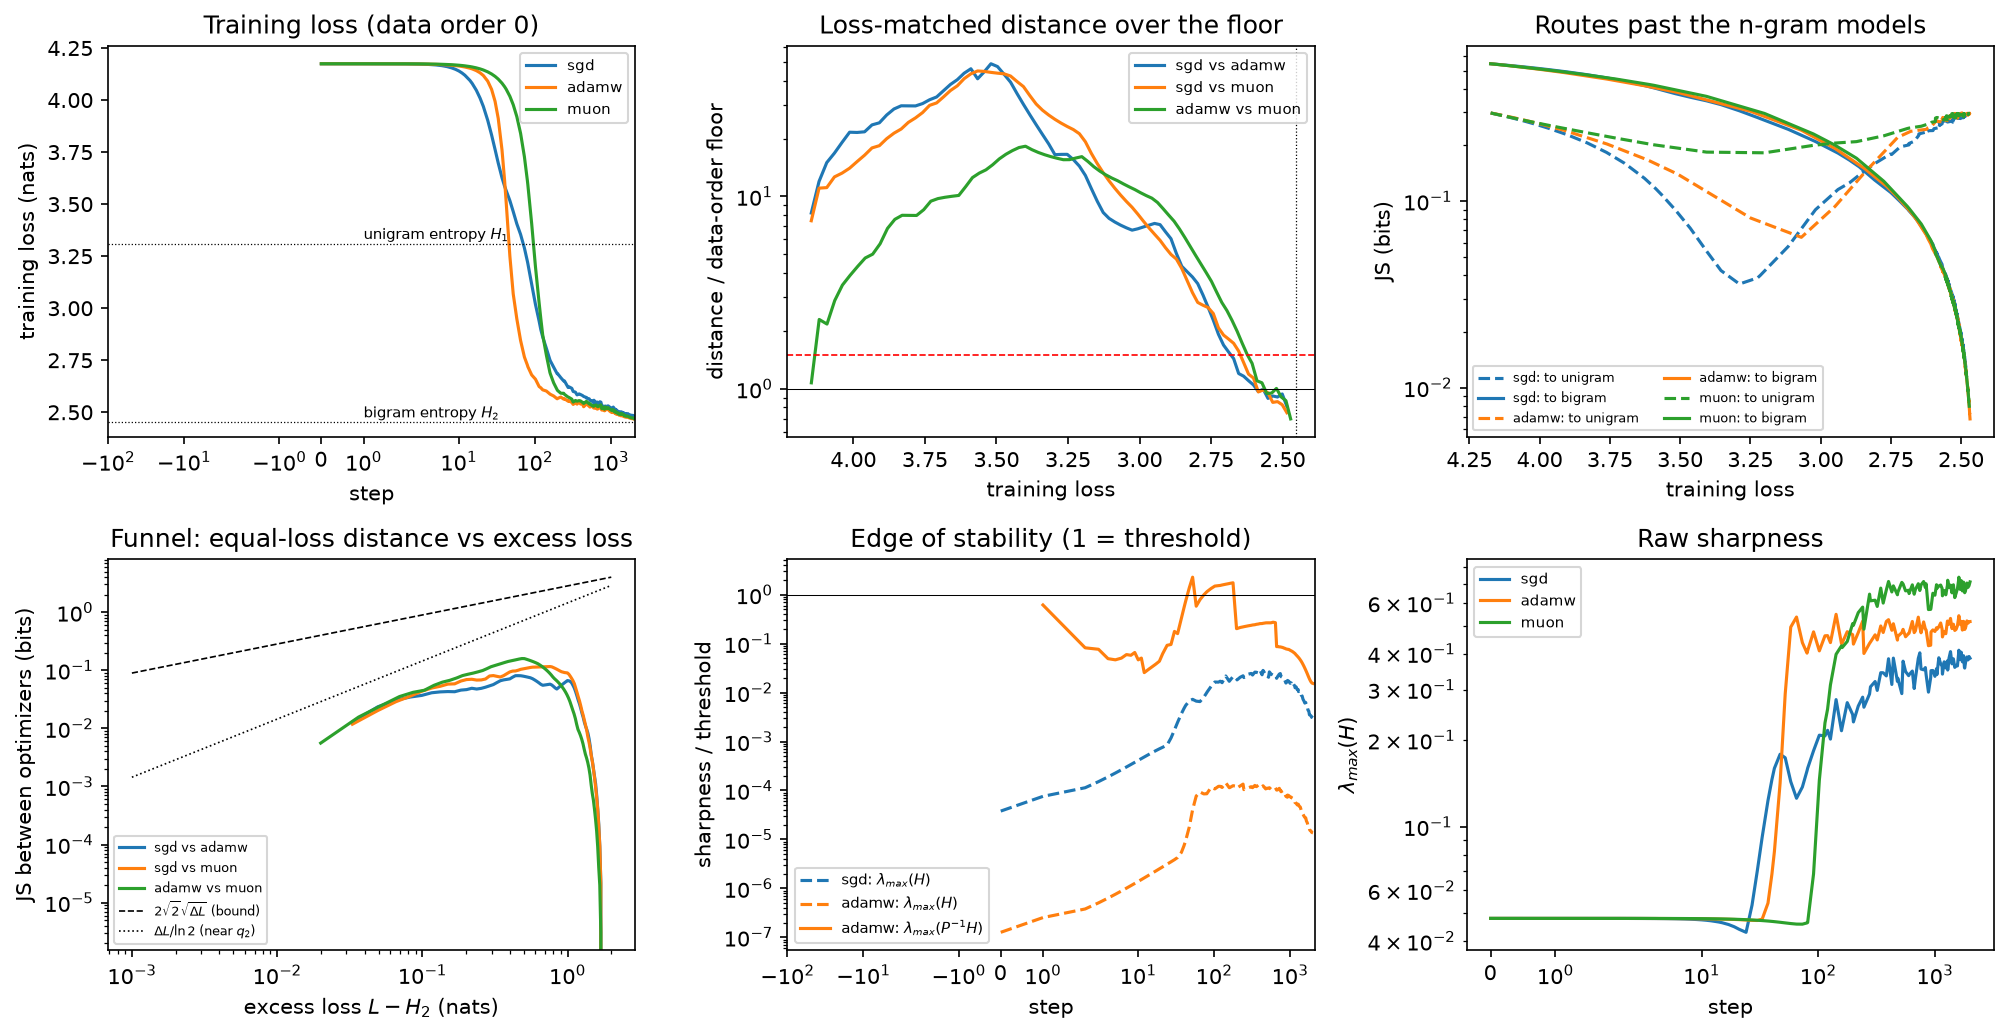
\includegraphics[width=\linewidth]{figures/toy/toy_model.png}\\[2pt]
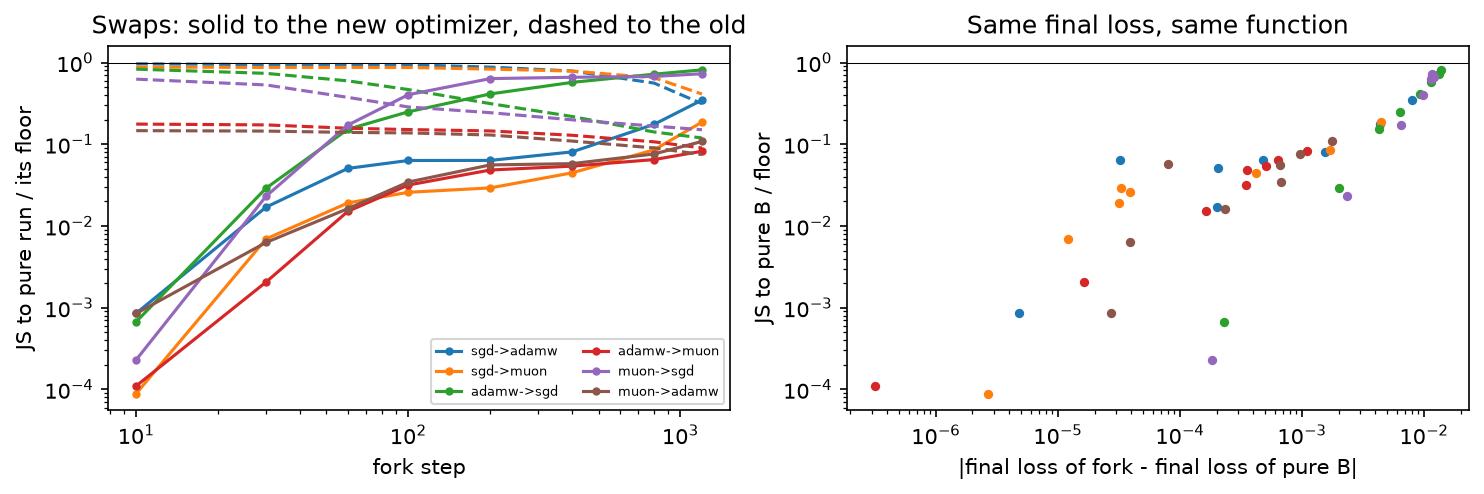
\includegraphics[width=0.75\linewidth]{figures/toy/toy_swaps.png}
%% PYTHONPATH=code python code/scripts/toy_model.py --text input.txt --out figures/toy
\caption{Toy model\extra: next-character logits $AB\,e_c+b$ for the previous character $c$ on Shakespeare
($V=65$, inner width 128, initialization $\mathcal N(0,0.02^2)$ for $A,B$ and $b=0$), batch 128, 2000 steps with
the schedule of the language models, learning rates from a sweep (SGD 0.3, AdamW 0.01, Muon 0.03 on $A,B$ with
AdamW at 0.01 on $b$), five data orders. Top: training loss with the unigram and bigram entropies; loss-matched
distance over the floor (red: 1.5; dotted: $H_2$); $\JS$ of the $d=0$ runs from the unigram (dashed) and bigram
(solid) models. Bottom: loss-matched $\JS$ between optimizers against the excess loss over $H_2$, with the two
bounds of \eqref{eq:funnel}; sharpness over its threshold; raw sharpness. Last row: swaps from $d=0$ at eight fork
steps, distance to pure $B$ (solid) and $A$ (dashed) in floors, and distance to pure $B$ against the gap
between the final losses.}
\label{fig:toy}
\end{figure}

\paragraph{The toy model.} Logits $AB\,e_c+b$ for the previous character $c$, trained on the bigram pairs of
Shakespeare (\cref{fig:toy}). The function is the $65\times65$ table of next-character distributions, all
losses are exact, and the class of reachable predictors is $\mathcal F_{\rm bigram}$, so its only funnel is the
bigram one. The bias plays the part of directions that are trained from the first step, the product $AB$ that of
directions that must first leave the saddle at zero. It reproduces the main observations: a loss-matched
distance up to 40 times the floor (18 for AdamW--Muon) that falls below 1.5 at loss 2.62--2.69 and ends below 1
at $H_2$, with no persistent split; the order in which the routes pass the unigram model; forks that end on the
optimizer they switch to; and barriers between optimizers well above those between data orders.

\paragraph{Routes before the funnel.} Near the initialization the gradient of the loss with respect to the
product is $G_0=-\sum_ap(a)(q(\cdot\mid a)-u)e_a^\top$, with $u$ uniform and $p$ the frequency of the context;
its top singular direction is close to the unigram direction $(q_1-u)p^\top$. With SGD, $b$ learns the unigram at
once and, for gradient flow from a small balanced initialization, each singular value of $AB$ grows as
$\dot s_k\approx2\sigma_ks_k$, with $\sigma_k$ the singular values of $G_0$ \citep{saxe2014exact}: exponentially,
at rates proportional to $\sigma_k$, so the modes are picked up one at a time, strongest first, and the route
passes through the unigram model before adding the bigram modes. Muon updates $A$ by $-\eta\,\mathrm{msign}(GB^\top)$
and $B$ by $-\eta\,\mathrm{msign}(A^\top G)$, which move every singular direction in the range of the gradient
at the same speed whatever $\sigma_k$: all modes of $AB$ grow together, the route heads for the spectrally
flattened target and stays away from the unigram model. AdamW normalizes each coordinate, which makes it free of
scale like Muon but in the coordinate basis: $b$ and $AB$ move at the same speed, and the route passes near the
unigram model, less closely than SGD's. In the toy the closest approach to the unigram model is 0.036 bits for
SGD, 0.064 for AdamW and 0.18 for Muon, the order measured on the Shakespeare transformers (0.001, 0.054, 0.111;
\cref{sec:res-route}). At this stage the mean gradient dominates the mini-batch noise. Two data orders of one
optimizer differ by a random walk, of squared size $\propto\eta^2t\sigma^2/B$ after $t$ steps, while two optimizers
drift apart linearly in $t$, so the ratio of their squared distances grows like $t$ times the squared
signal-to-noise ratio of the gradient: the ratio to the floor is largest before the funnel, as in
\cref{fig:overview}.

\paragraph{Proposition 2 (the floor near the funnel).} Near $q_s$ write each run's function as
$\pi=q_s+\mu_X+\xi_X^d$, with $\mu_X$ common to all data orders of optimizer $X$ and $\xi^d_X$ a zero-mean part
due to data order $d$. To second order $\JS(\pi,\pi')=\frac1{8\ln2}\|\pi-\pi'\|_F^2$ in bits, with
$\|\delta\|_F^2=\mathbb E_s\sum_y\delta(y\mid s)^2/q_s(y\mid s)$, so
\begin{equation}
F_X=\tfrac1{4\ln2}\mathbb E\|\xi_X\|_F^2,\quad
C_{\rm other}=\tfrac{F_A+F_B}2+\tfrac1{8\ln2}\|\mu_A-\mu_B\|_F^2,\quad
C_{\rm same}=C_{\rm other}-\tfrac1{4\ln2}\mathbb E\langle\xi^d_A,\xi^d_B\rangle_F,
\label{eq:decomp}
\end{equation}
for the floor $F_X$ and the cross distances on other and on the same data orders. The cross distance over the
larger floor is therefore at most about one plus the optimizer's own term $\frac1{8\ln2}\|\mu_A-\mu_B\|_F^2$ over
the floor, and below one when two optimizers respond alike to the same batches. The measurements at equal steps
(\cref{sec:res-route}) fit this: for AdamW--Muon on TinyStories-30M at step 20{,}000, $C_{\rm other}=0.0556$ bits
exceeds the mean of the floors (0.0547, 0.0512) by 0.0027, 5\% of the floor, and $C_{\rm same}=0.0511$; at step
10{,}000 the excess is 0.0039 (5\%), and on TinyStories-10M at step 10{,}000 it is 0.0037 (6\%) with
$C_{\rm same}=0.0574$ against 0.0632. In the toy the excess is 6\% of the floor. Over training the excess shrinks
as the funnel predicts: on TinyStories it is 8--10 times the mean floor at step 30, 0.3--0.4 times at step 120 and
about 0.1 by step 1000, and 4--7\% from there on (at equal steps; on Shakespeare, where Muon memorizes faster, it
stays near 50\%). Most of the distance between two optimizers is data-order noise, and part of it is shared
when they see the same batches.

\paragraph{Swaps.} A fork from $A$ to $B$ is a run of $B$ from another starting point. In the regime of
Proposition~2 it differs from pure $B$ on the same data order through its mean part, which the loss bounds, so it
lands on $B$ once it reaches $B$'s loss, that is whenever $B$ is fast enough to get there in the remaining steps,
and otherwise keeps a loss, and with it a function, set by the parent's progress. In the toy every optimizer
reaches $H_2$, all forks end within 0.81 floors of pure $B$, and the distance to pure $B$ grows with the gap
between the final losses (\cref{fig:toy}, last row). In the transformers SGD is the one optimizer too slow to undo
its parent's progress, and the forks into it are the ones that stay near their parent (\cref{sec:res-swap}).

\paragraph{Weight space.} The function $AB+b$ is unchanged by $(A,B)\mapsto(AR,R^{-1}B)$ for invertible $R$, and
by any change of $A$ and $B$ that leaves their product unchanged: each function is a high-dimensional fiber of
weights. Gradient flow conserves $A^\top A-BB^\top$ \citep{du2018balanced}, so SGD from a small initialization
stays near the balanced point of the fiber, which minimizes $\|A\|_F^2+\|B\|_F^2$ for its product
($\|A\|_F^2+\|B\|_F^2\ge2\|AB\|_*$, with equality for balanced factors). Normalized updates do not conserve it
and end elsewhere on the fiber. Two points of one fiber compute the same function, but the segment between them
leaves it, since $(\alpha A_1+(1-\alpha)A_2)(\alpha B_1+(1-\alpha)B_2)\ne A_1B_1$ in general, so a loss barrier
between optimizers is compatible with equal functions. In the toy the imbalance $\|A^\top A-BB^\top\|_F/\|A^\top
A\|_F$ is 0.39 (SGD), 0.91 (AdamW) and 2.1 (Muon), SGD has the smallest $\ell_2$ norm (27, against 43 for AdamW
and 36 for Muon), and the barriers between optimizers on one data order (0.013--0.024 nats) are 20--50 times
those between data orders of SGD or AdamW, at a function distance below the floor. This is the parameter-space
implicit bias of the asymptotic theory acting along the fiber rather than on the function, and it accounts for
the weights carrying each optimizer's geometry and for the barriers between AdamW and Muon while their functions
agree (\cref{sec:res-swap,sec:res-metrics}).

\paragraph{Break-even points by optimizer.} \citet{jastrzebski2020breakeven} model the early phase by one
quadratic direction whose curvature grows until the step becomes unstable along it. Where this happens depends
on how the update scales with the gradient.
(i) SGD with momentum is linear in the gradient; along an eigenvector of $H$ with eigenvalue $\lambda$ it is
stable if and only if $\eta\lambda<2+2\mu$, so its break-even sharpness is $(2+2\mu)/\eta$, lower for larger
rates (their first conjecture).
(ii) AdamW is linear in the gradient only for a frozen preconditioner, and $P$ changes over about
$1/(1-\beta_2)$ steps. The threshold applies to $\lmax(P^{-1}H)$ \citep{cohen2022adaptive}, so the raw sharpness at
break-even is about $38\,p/\eta$, with $p$ the preconditioner along the sharp direction, of the size of the
gradient's root mean square. On TinyStories-30M $\lmax\approx5$ at $\eta=1.5\times10^{-3}$ gives $p\approx2\times10^{-4}$,
and AdamW sits at the lowest raw sharpness of the three (5--10, against 12--20 for Muon and 20--30 for SGD;
\cref{fig:app-sharpness}). A growing oscillation also raises $v$ and with it $P$, so AdamW stabilizes itself
through its preconditioner as well as through the curvature. The test is whether, at the steps at which AdamW
is at its threshold after warmup, $\lmax\eta$ grows with the gradient: at the tuned rate, over those steps of
the five data orders, a log-log fit of $\lmax\eta$ against the gradient norm has slope 1.15 on TinyStories-30M
(77 steps, $r=0.82$) and 1.61 on TinyStories-10M (69 steps, $r=0.89$), and on Shakespeare the relation is weak
(31 steps, $r=0.52$). These are slopes against the gradient norm at one rate, not against $\eta$ (for which see
\cref{sec:res-coincide}). The dependence on the gradient holds, with a slope above the predicted 1: the global gradient norm is only a proxy for $p$, which is set where
the direction lies, on TinyStories mostly in the embeddings (\cref{fig:anatomy-layers}).
(iii) Muon's update $\mathrm{msign}(M)$ does not change when the gradient is scaled, so it has no linear regime,
and its threshold is not on $\lmax(H)$. On a quadratic $\frac\lambda2\|X\|_F^2$ in a matrix $X$, without
momentum, $X\leftarrow X-\eta\,\mathrm{msign}(X)$ maps each singular value $s$ to $|s-\eta|$: the iterates enter
$\{\|X\|_2\le\eta\}$ and stay there for every $\lambda>0$. No curvature makes Muon diverge; the curvature sets
only the excess loss of the oscillation, at most $\frac\lambda2\eta^2\operatorname{rank}X$. The iterates still
settle at an edge of stability, but one set by the gradient. For a step $-\eta U$ with $\|U\|_2=1$ and
$\langle G,U\rangle=\|G\|_*$, the nuclear norm, as $U=\mathrm{msign}(G)$ gives, the loss changes to second order
by $-\eta\|G\|_*+\frac12\eta^2\langle U,H[U]\rangle$, which is negative only while the curvature along the update is
below $2\|G\|_*/\eta$. \citet{islamov2026noneuclidean} show that the stability condition of such scale-invariant
updates bounds a sharpness measured in the spectral norm by $2\|\nabla L\|_*/\eta$, and that full-batch spectral
gradient descent sits at this bound. Muon's break-even point is thus set by this spectral-norm sharpness, which we
have not yet measured, rather than by $\lmax(H)$; on the part left to its auxiliary AdamW it is AdamW's
(\cref{sec:method-aux}). Across learning rates, Muon's $\lmax(H)$ falls about as $1/\eta$, like the thresholds of
the other two (\cref{sec:res-coincide}).

\paragraph{Why the break-even point does not decide the function.} Stability caps the curvature along the
few sharpest directions of each optimizer's operator. This moves the run along the fiber of weights and sets how
fast the loss falls, but it does not choose between functions with the same loss: by Proposition~1, a function in
a stage class is pinned by its loss up to the excess loss. An oscillation of amplitude $a$ along the sharpest
direction costs $\frac12\lambda a^2$ of loss, so it moves the function no more than that excess allows, and
equally in floor pairs and in cross pairs. This is why the edge-of-stability events (AdamW at its threshold for
much of training, SGD only early) do not line up with changes in the loss-matched distance
(\cref{sec:res-coincide}), and why on CIFAR-10 the break-even effects on sharpness and gradient noise replicate
while two learning rates stay within 1.75 floors at equal loss (\cref{sec:res-breakeven}).

\paragraph{Predictions.} A persistent split needs a class without a best element, as when training into
interpolation; AdamW and Muon memorize Shakespeare without splitting, so either their implicit biases agree on
held-out text or the runs are not yet in that regime. Across learning rates the sharpness of SGD and AdamW should
scale as $1/\eta$; in the sweeps it does, and so does Muon's $\lmax(H)$ (\cref{sec:res-coincide}). Whether Muon
sits at its spectral-norm threshold is still to be measured (\cref{sec:discussion}).

%% =================================================================
\section{Discussion and limitations}
\label{sec:discussion}
%% =================================================================

\paragraph{No split after warmup.} The hypothesis of the title, that optimizers first follow one path and
separate later, is not what we observe. After warmup, at equal training loss, two optimizers on the same data
order are about as far apart as one optimizer on two data orders, down to the lowest loss we reach. The
exceptions involve SGD: on TinyStories-10M it is up to about 1.5 times as far from AdamW or Muon at losses
4--2.5 and within 1.1 times below, and on Shakespeare, where it barely trains, it stays above the floor, with the
only persistent split, against Muon, a fragile one. Within warmup the ratios to the floor are large, but there the
runs still share their initialization and the floor is near zero, so these ratios are inflated; in this stage
the optimizers pick up simple statistics in different orders (on Shakespeare SGD and AdamW pass through the
unigram model and Muon does not). After it the function is set mostly by the data, and the optimizer matters
mainly through speed (\cref{sec:theory} makes this precise). This rests on comparing at equal loss: at equal
steps all pairs look different for most of training, Muon being faster than AdamW throughout, and on Shakespeare
Muon's faster memorization dominates the comparison.

\paragraph{What the floor means.} Being within the floor does not mean computing the same function: at the end
of the TinyStories runs two data orders of AdamW or Muon differ by 0.051--0.062 bits. The finding is that changing the optimizer
perturbs the learned function no more than changing the order of the data or, where we tested it, the
initialization (\cref{sec:res-controls}), not that it does not perturb it. The asymptotic implicit-bias results
\citep{gunasekar2018geometry,zhang2024adam,fan2025spectral} describe the limit of long training of linear models
on separable data. Our TinyStories models see at most 1.2 epochs, and by then the loss-matched difference
between optimizers is within the data-order noise; in the linear control the split appears only near
interpolation. Nor do the swaps show an early decision: a fork ends at the function of the optimizer it switches
to whenever that optimizer is fast enough to get there in the remaining steps (on TinyStories, whenever it is the
faster one, at every fork step we tried), and keeps the mark of its parent only when the new optimizer is too slow
to move away from it.

\paragraph{Function space and weight space.} The mode-connectivity barriers tell a different story from the
function distances. After a change of optimizer a fork needs a later fork step to stay linearly connected to its
parent than after a change of data order, except for Muon on Shakespeare, which is itself unstable to the data
order while it memorizes. Between pure runs the size of the barrier does not single out the
optimizer (AdamW and Muon are further apart than two data orders only on TinyStories-10M), but its location does:
the barrier between AdamW and Muon extends into the middle blocks, while that between two data orders lies in the
first block, although their functions are as close. Different optimizers thus reach functions that are
equivalent up to data-order noise through weights that differ beyond the first block, whereas data orders differ
mainly in the first. The weights
also carry the geometry each optimizer is biased towards: more even entries for AdamW than for SGD, and more even
singular values for Muon (\cref{sec:res-metrics}), and after a swap that geometry is a mixture weighted by
how far each optimizer moved the weights, even when the function is entirely the second optimizer's. The hidden
states sit in between: on TinyStories AdamW and Muon differ after the first block and little after the others. Part of the barriers may be scale: the optimizers move the
weights by very different amounts (on TinyStories Muon's end 5--6.6 initial norms from the initialization, AdamW's
2.7--2.8 and SGD's 0.4--0.6), and interpolating between weights of different scales can raise the loss without any
change in function.

\paragraph{Break-even point.} On CIFAR-10 we reproduce the sharpness and gradient-noise effects of
\citet{jastrzebski2020breakeven}, but the separation of trajectories between learning rates is mostly a
difference in speed: at equal loss, 0.01 and 0.1 stay within 1.75 times the floor. Comparing at equal steps
overstates how differently two training procedures shape the function.

\paragraph{Edge of stability.} On TinyStories AdamW is at its adaptive edge of stability through much of
training whether or not the optimizers differ, and SGD meets its threshold only early in training; neither
explains the start or the end of the early episode, which ends within warmup in all pairs but one and in the same
way for AdamW and Muon. With the cosine schedule the threshold acts as a ceiling: once the learning rate decays,
the sharpness levels off instead of following the threshold up, and the runs leave the edge of stability. Across
learning rates the top Hessian eigenvalue falls about as $1/\eta$ for all three optimizers, Muon included, whose
threshold is on a spectral-norm sharpness \citep{islamov2026noneuclidean}. The one edge-of-stability event that lines up with a change in function, Muon's
auxiliary AdamW overshooting its threshold just before Muon memorizes on Shakespeare, is not what drives the
memorization, which persists in the matched control (where the overshoot comes later and is smaller). The
anatomy adds that the sharp direction is optimizer-specific, lies at the input end of the network, and, except in
AdamW's embeddings, mostly comes from curvature between layers, but its changes do not line up with changes in
function distance either.

\paragraph{Future work.} Two sets of runs are still in progress: Muon's spectral-norm sharpness, to test whether
Muon sits at the threshold $2\|\nabla L\|_*/\eta$ of \citet{islamov2026noneuclidean}, and break-even runs of the
three optimizers at a constant learning rate, as in \citet{jastrzebski2020breakeven}, without our warmup and
cosine decay. Beyond them: whether the sharp direction moves to the new optimizer's layers after a swap, and
whether lowering the learning rate of only those layers changes the function.

\paragraph{Limitations.}
\begin{itemize}
\item The noise floor varies only the data order; a second initialization (\cref{sec:res-controls}) gives the same
  distance as a new data order, but only two of each were run, on Shakespeare and TinyStories-10M.
\item Learning rates come from five-point sweeps on one data order, and the Shakespeare AdamW rate is the
  smallest of its grid. The other rates of the sweeps agree with the tuned ones on TinyStories
  (\cref{fig:lr-robust}), but only against the tuned runs' floor. SGD trains poorly at the stable rates on Shakespeare, so comparisons with SGD there stop
  at loss 2.61, and its large data-order noise on TinyStories makes ``no split'' against SGD a weak statement.
\item The first exceedance is degenerate (\cref{sec:method-split}); episodes and the persistent split depend on
  the margin $m_\times$, the run length $k$ and the matching tolerance $\tau$; the conclusions hold over the
  variants we tried (\cref{sec:res-split}), except the Shakespeare Muon--SGD split.
\item The loss grid ends at the lowest loss that all runs of a pair reach, so a split below it would be missed.
\item The thresholds are those of linear stability on a quadratic with a frozen preconditioner; Muon's threshold
  is on a spectral-norm sharpness that we have not yet measured (\cref{sec:theory}), and the AdamW ratio at the
  first steps reflects a preconditioner built from few gradients.
\item The sweeps with sharpness use one data order and three or four rates per optimizer.
\item Sharpness is measured on the training loss of a fixed batch of 32 training sequences with 20 Lanczos
  iterations, in float32 with TF32 matrix products, while training uses bfloat16 autocast and the predictions are
  compared on held-out validation contexts.
\item Loss matching and the mode-connectivity barrier use a training probe of 64 sequences.
\item The landing coordinate is a ratio of distances, not a projection onto the segment between the pure
  runs.
\item The models are small (up to 30M parameters) and trained for at most 655M tokens.
\end{itemize}

%% =================================================================
\section{Conclusion}
\label{sec:conclusion}
%% =================================================================

From the same initialization and data order, SGD with momentum, AdamW and Muon do not first share a path and
then split. After warmup, at equal training loss, two optimizers are about as far apart as two data orders of one
optimizer. This holds in all three language-model settings, with SGD up to about 1.5 times as far from AdamW or
Muon at losses 4--2.5 on TinyStories-10M, every pair within 1.1 times on TinyStories-30M, and one short AdamW--Muon
episode on Shakespeare; the exceptions are the pairs with SGD on Shakespeare, where SGD barely trains, with the
only persistent split, Muon--SGD, a fragile one. The large ratios within warmup are inflated by a floor near zero.
Muon is faster than AdamW, and at equal steps the two are at most about a fifth closer on the same data order than
two data orders of one optimizer, because they share their recent batches; at the end of TinyStories-30M,
replacing AdamW by Muon changes the function no more than reshuffling the data. Neither the edge of stability nor
the end of warmup explains the changes in distance. Switching optimizers during training does not reveal an early decision either: the run ends at the
function of the optimizer it switches to whenever that one is fast enough to get there, on TinyStories whenever
it is the faster one, even late in training. The optimizer does
leave a mark in weight space: after a change of optimizer a fork usually needs a later fork step to stay
linearly connected to its parent, the barrier between AdamW and Muon extends beyond the first block, where that
between two data orders lies, and the weights carry each optimizer's geometry, mixed after a swap according to
how far each moved them. On TinyStories the hidden representations differ after the first block and little after
the others, and the functions no more than with another data order even off the data distribution. As a check,
on TinyStories every rate of the sweeps that trains stably is within 0.8--1.1 floors of the tuned runs, with one
exception at 1.35, and on TinyStories-10M rates from a quarter to four times each optimizer's rate stay within
0.8--1.1 times the floor of the tuned runs at equal loss.
A linear model on separable data, where the limits of training are known to differ, shows that our test can
detect a split, and places it near interpolation; but AdamW and Muon trained on Shakespeare until they memorize
the training set do not split either, so for these models the absence of a split is not only a matter of
training too briefly. A simple model accounts for this pattern (\cref{sec:theory}): at equal loss, functions of
one n-gram class are pinned by their excess loss whatever the optimizer, while the optimizer chooses the route,
the speed, the weights among those computing a function, and a cap on the curvature, which for Muon applies to a
spectral-norm sharpness.

\printbibliography

%% =================================================================
\clearpage
\appendix
\section{Hyperparameters}
\label{app:hparams}
%% =================================================================

\begin{table}[ht]
\centering\small
\caption{Optimizer hyperparameters, shared by all language-model settings unless noted. The Shakespeare control
matches Muon's auxiliary AdamW to AdamW: $\beta=(0.9,0.99)$, weight decay 0.1, learning rate $3\cdot10^{-4}$.}
\label{tab:optim}
\begin{tabular}{@{}lp{0.27\linewidth}p{0.27\linewidth}p{0.27\linewidth}@{}}
\toprule
 & SGD & AdamW & Muon \\
\midrule
Update & heavy ball, $\mu=0.9$, not Nesterov & $\beta=(0.9,0.95)$; Shakespeare $(0.9,0.99)$; $\epsilon=10^{-8}$ &
  Nesterov momentum $0.95$; 5 Newton--Schulz steps (bfloat16); scale $\sqrt{\max(1,n_{\rm out}/n_{\rm in})}$ \\
Parameters & all & all & matrices in transformer blocks; auxiliary AdamW ($\beta=(0.9,0.95)$, $\epsilon=10^{-8}$) on
  embeddings, head, gains \\
Weight decay & none & 0.1 on tensors with $\ge2$ dims, none on gains & none (Muon and auxiliary AdamW) \\
Clipping & none & none & none \\
\bottomrule
\end{tabular}
\end{table}

\begin{table}[ht]
\centering\small
\caption{Learning-rate sweeps (data order 0, five rates per optimizer). Rates used in the main runs in bold.
Selection: final validation loss for TinyStories, minimum validation loss over training for Shakespeare. The
auxiliary AdamW of Muon keeps the learning rate of \cref{tab:setup} throughout the sweep. SGD ($\dagger$: best
on data order 0) uses a lower rate, since its best rate diverged or blew up on other data orders: 0.2 on
Shakespeare (orders 1 and 2), 0.1 on TinyStories-10M (orders 1--3) and 0.3 on TinyStories-30M (orders 2--4).}
\label{tab:sweep}
\begin{tabular}{@{}llll@{}}
\toprule
Setting & SGD & AdamW & Muon \\
\midrule
Shakespeare-char & \textbf{0.05}, 0.1, 0.15, 0.2$^\dagger$, 0.25 & $\mathbf{3\cdot10^{-4}}$, $10^{-3}$, $2\cdot10^{-3}$,
  $4\cdot10^{-3}$, $8\cdot10^{-3}$ & 0.005, 0.01, 0.02, \textbf{0.04}, 0.08 \\
TinyStories-10M & \textbf{0.03}, 0.1$^\dagger$, 0.3, 1, 3 & $3\cdot10^{-4}$, $10^{-3}$, $\mathbf{2\cdot10^{-3}}$,
  $4\cdot10^{-3}$, $8\cdot10^{-3}$ & 0.005, \textbf{0.01}, 0.02, 0.04, 0.08 \\
TinyStories-30M & 0.03, \textbf{0.1}, 0.3$^\dagger$, 1, 3 & $3\cdot10^{-4}$, $10^{-3}$, $\mathbf{2\cdot10^{-3}}$,
  $4\cdot10^{-3}$, $8\cdot10^{-3}$ & 0.005, \textbf{0.01}, 0.02, 0.04, 0.08 \\
\bottomrule
\end{tabular}
\end{table}

\begin{table}[ht]
\centering\small
\caption{Fork steps of the swaps (all six ordered pairs, plus each optimizer into itself with data order 1).}
\label{tab:forks}
\begin{tabular}{@{}ll@{}}
\toprule
Setting & Fork steps \\
\midrule
Shakespeare-char & 25, 50, 100, 200, 300, 450, 600, 800, 1000 \\
TinyStories-10M & 50, 100, 200, 400, 700, 1000, 1500, 2500, 4000 \\
TinyStories-30M & 100, 200, 400, 800, 1400, 2000, 3000, 5000, 8000 \\
\bottomrule
\end{tabular}
\end{table}

Break-even runs: plain SGD (momentum 0), constant learning rate, no warmup. CIFAR-10: 100 epochs, i.e.\
39{,}000 steps at batch 128, 166{,}600 at batch 30 and 16{,}600 at batch 300; data orders 0 and 1.
Shakespeare and TinyStories-10M: 1{,}500 and 10{,}000 steps at their training batch size, learning rates 0.03,
0.1 and 0.3; data orders 0, 1 and 2.

%% =================================================================
\section{Measurement details}
\label{app:measure}
%% =================================================================

A grid ``every $N$ + $K$ log'' is $\{0,N,2N,\dots\}\cup\{\mathrm{round}(T^{u}):u\in\text{$K$ evenly spaced
values in }[0,1]\}\cup\{T\}$, i.e.\ the union of a linear grid and $K$ log-spaced steps between 1 and $T$.

\begin{table}[ht]
\centering\small
\caption{Logging grids, probe sizes and measurement settings of the main language-model runs (forks inherit their parent's) and of the CIFAR-10 runs at batch 128.
Fixed sets of examples are drawn once, from random streams separate from the training batches, and are the
same for all runs of a setting.}
\label{tab:grids}
\begin{tabular}{@{}lllll@{}}
\toprule
 & Shakespeare-char & TinyStories-10M & TinyStories-30M & CIFAR-10 (batch 128) \\
\midrule
Prediction steps $\cS$ & every 50 + 40 log & every 250 + 30 log & every 500 + 30 log & every 390 + 40 log \\
Checkpoints & every 250 + 12 log & every 1000 + 12 log & every 2000 + 12 log & every 3900 + 12 log \\
Measurement steps $\cM$ & every 50 + 30 log & every 500 + 30 log & every 1000 + 30 log & every 390 + 30 log \\
Validation probe ($N$) & $64\times256=16{,}384$ & $128\times16=2{,}048$ & $128\times16=2{,}048$ & 10{,}000 images \\
Training probe & 64 seq.\ (16{,}384 tok.) & 64 seq.\ (16{,}384 tok.) & 64 seq.\ (16{,}384 tok.) & 2{,}000 images \\
Hessian batch $\mathcal H$ & 32 seq.\ (8{,}192 tok.) & 32 seq.\ (8{,}192 tok.) & 32 seq.\ (8{,}192 tok.) & 2{,}500 images \\
Lanczos iterations & 20 & 20 & 20 & 20 \\
Batch sharpness & $8\times64$ seq. & $8\times128$ seq. & $8\times128$ seq. & $8\times128$ images \\
$\hat K$ (break-even runs) & $25\times64$ seq. & $25\times128$ seq. & -- & $25\times128$ images \\
\bottomrule
\end{tabular}
\end{table}

\paragraph{Sharpness.} Lanczos runs for 20 iterations with full reorthogonalization (two Gram--Schmidt passes
per iteration) from a fixed Gaussian start, and returns the top Ritz pair. Hessian-vector products use double
backpropagation through one gradient graph, with the exact (math) attention kernel, in float32 without
autocast but with TF32 matrix products, on the model before the update of the measured step.

\paragraph{Split.} $\tau=0.02$, $m_\times=0.5$, $m_+=0$, $k=3$, 1000 bootstrap resamples. The training loss
of a run is its loss on the training probe at its prediction steps.

\paragraph{Mode connectivity.} Barrier on the 64 sequences of the training probe, at 11 evenly spaced values
of $\alpha$, between final checkpoints.

\paragraph{Prediction trajectories.} Break-even runs: 128 evenly spaced probe positions; top 50 principal
components of the centered probability vectors, then UMAP. \Cref{fig:div,fig:traj-lr}: densMAP of the $\sqrt{\JS}$
distance between all pairs of logged steps (\cref{sec:method-distance}).

\subsection{Function metrics}
\label{app:metrics}


The metrics are computed on 1024 fixed validation examples (sequences or test images), drawn separately
from the probe and shared by all runs; the input-derivative metrics use the first 32.

\paragraph{Input derivatives.} Let $f(x)$ be the loss at the true labels as a function of the input $x$. For
the language models $x\in\mathbb R^{64\times d}$ is the token-embedding matrix of the first 64 tokens of a
sequence (position embeddings are added inside the model) and $f$ is the mean next-token cross-entropy over
these 64 positions; for the CNN $x$ is the normalized image and $f$ its cross-entropy. With $g=\nabla f(x)$,
$H=\nabla^2f(x)$ and $T[u,u,\cdot]=\nabla_x\big(u^\top H(x)u\big)$, and $z_1,\dots,z_8$ standard Gaussian
probes:
\begin{itemize}
\item gradient norm $\|g\|$;
\item Jacobian norm $\|J\|_F$ of the softmax output with respect to $x$ \citep{novak2018sensitivity}: exact
  for the CNN (one vector-Jacobian product per class), and estimated as
  $\big(\frac18\sum_j\|J^\top z_j\|^2\big)^{1/2}$ over the $64\times V$ outputs for the language models;
\item Hessian norm $\|H\|_F\approx\big(\frac18\sum_j\|Hz_j\|^2\big)^{1/2}$;
\item top input-Hessian eigenvalue $\lambda_x=v^\top Hv$, with $v$ from 20 power iterations (the eigenvalue
  of largest magnitude) \citep{moosavi2019cure};
\item level-set curvature $\big(\frac18\sum_j\|PHPz_j\|^2\big)^{1/2}/\|g\|\approx\|PHP\|_F/\|g\|$, with
  $P=I-\hat g\hat g^\top$ the projection orthogonal to the gradient, a projected variant of the normalized
  curvature of \citet{srinivas2022lowcurv};
\item third order: the norm $\|T\|_\sigma=\max_{\|u\|=1}T[u,u,u]$, by shifted symmetric power iteration
  $u\leftarrow(T[u,u,\cdot]+\alpha u)/\|T[u,u,\cdot]+\alpha u\|$ with $\alpha=\|T[u_0,u_0,\cdot]\|$, 20
  iterations, best of 3 random starts (as $T[u,u,u]$ is odd in $u$, this is also $\max|T[u,u,u]|$); the
  third derivative along the sharpest direction $T[v,v,v]$, with the sign of $v$ fixed by $v^\top g\ge0$; and
  the curvature length $|\lambda_x|/\|T[v,v,\cdot]\|$, the distance over which, to first order, $\lambda_x$
  changes by its own size (for a simple eigenvalue $\nabla_x\lambda_x=T[v,v,\cdot]$).
\end{itemize}
Each is reported as mean and standard deviation over the 32 points.

\paragraph{Weight norms.} Over all parameters $\theta$: $\ell_0$ (entries with $|\theta_i|>10^{-8}$),
$\ell_1$, $\ell_2$, $\ell_3$, $\ell_\infty$. For each weight tensor with at least two dimensions, reshaped
to a matrix $W$ (output $\times$ input): the spectral norm $\|W\|_2$, nuclear norm $\|W\|_*$ and stable rank
$\|W\|_F^2/\|W\|_2^2$ \citep{sanyal2020stable}. Distance from initialization $\|\theta-\theta_0\|_2$, also
relative to $\|\theta_0\|_2$ \citep{nagarajan2019distance}. The log spectral complexity
$\log\big(\prod_i\|W_i\|_2\cdot(\sum_i(\|(W_i-W_i^0)^\top\|_{2,1}/\|W_i\|_2)^{2/3})^{3/2}\big)$ of
\citet{bartlett2017spectral}, with the initialization as reference matrices. For the CNN only, the path norm
as computed by \citet{jiang2020fantastic} \citep[after][]{neyshabur2015norm}: the sum of the outputs on an
all-ones input of the network with every parameter squared and identity activations.

\paragraph{Accuracy and robustness.} Accuracy on the 1024 validation examples (for the language models, next-
token accuracy over all positions). For the CNN, accuracy under Gaussian input noise of standard deviation
0.05, 0.1 and 0.2 (in normalized pixel units) \citep{ford2019noise}. For the language models, a one-token
substitution sensitivity after \citet{hahn2021sensitivity}: for 32 validation contexts of 64 tokens, we
replace each position in turn by a uniformly random different token and count how many of the 64
substitutions change the argmax prediction at the last position; we report this count as a fraction of 64,
averaged over contexts.
All derivatives are taken by automatic differentiation in float32, with the exact (math) attention kernel.

%% =================================================================
\section{Compute}
\label{app:compute}
%% =================================================================

All runs used one NVIDIA L40S GPU each on the MIT ORCD cluster. The project took 103 GPU-hours in all, 60\% of
them for the forks (\cref{tab:compute}), and 89 CPU core-hours for the offline analyses that run on CPU (mode
connectivity, representations, off-distribution distances, swap landing and the split statistics). Twelve smoke-test runs (0.2 GPU-hours) are
not counted. The GPU-hours include runs that were later replaced and are not in the run counts (SGD at its best
sweep rate on data orders 1--4, which diverged), and the Shakespeare break-even count includes the three runs at
rate 1.0, which diverged. Not in the table are the learning-rate runs of \cref{fig:traj-lr} (12 runs on
TinyStories-10M) and the sweeps with sharpness measurements (10 runs on TinyStories-10M, 15 on Shakespeare).

\begin{table}[ht]
\centering\small
\caption{Runs per suite and compute. The matched-Muon control has one more run, on data order 0, that saves the
fork checkpoints for the sharpness of the auxiliary block (\cref{sec:method-aux}).}
\label{tab:compute}
\begin{tabular}{@{}lrr@{}}
\toprule
Suite & Runs & GPU-hours \\
\midrule
Learning-rate sweeps (3 settings) & $3\times15$ & 9.0 \\
Main runs (3 settings) & $3\times15$ & 16.7 \\
Forks (3 settings) & $3\times81$ & 61.1 \\
Break-even, Shakespeare and TinyStories-10M & $12+9$ & 2.6 \\
Break-even, CIFAR-10 & 10 & 1.1 \\
Shakespeare control (matched Muon)\extra & $5+1$ & 0.5 \\
Second initialization, Shakespeare and TinyStories-10M\extra & $2\times6$ & 1.0 \\
Shakespeare trained into memorization\extra & 10 & 0.5 \\
Offline function metrics & -- & 10.7 \\
\midrule
Total & 392 & 103.2 \\
\bottomrule
\end{tabular}
\end{table}

%% =================================================================
\FloatBarrier
\section{Additional figures and tables}
\label{app:figures}
%% =================================================================

\begin{table}[ht]
\centering\small
\caption{Edge of stability in the language models: end of warmup $w$; measured steps at the edge of stability
($\mathcal Q\ge0.9\,\Theta$; $\lmax$ for SGD, preconditioned sharpness for AdamW) of the $d=0$ run, from first
to last; onset $s_{\rm EoS}$ over the 5 data orders; fraction of measured steps at the edge of stability over
the 5 data orders; first exceedance $t^\ast_X$ of the $d=0$ run against the other two optimizers (in the order
SGD, AdamW, Muon); and its persistent split, if any.}
\label{tab:coincide}
\setlength{\tabcolsep}{4pt}
\begin{tabular}{@{}llcccccc@{}}
\toprule
Setting & Run & $w$ & at EoS ($d=0$) & $s_{\rm EoS}$ (all $d$) & fraction of $\cM$ & $t^\ast_X$ & $t^\ast_{{\rm p},X}$ \\
\midrule
Shakespeare     & SGD   & 100 & 21--120   & 21     & 2--14\%  & 1 / 1 & 191 (vs Muon) \\
                & AdamW & 100 & 1--500    & 1      & 11--16\% & 1 / 1 & -- \\
                & Muon  & 100 & --        & --     & --       & 1 / 2 & 14 (vs SGD) \\
TinyStories-10M & SGD   & 200 & 62--1500  & 45--500 & 6--12\% & 3 / 1 & -- \\
                & AdamW & 200 & 1--4500   & 1      & 50--65\% & 1 / 1 & -- \\
                & Muon  & 200 & --        & --     & --       & 1 / 7 & -- \\
TinyStories-30M & SGD   & 400 & 60--658   & 60--467 & 10--16\% & 2 / 1 & -- \\
                & AdamW & 400 & 1--14000  & 1      & 40--69\% & 1 / 1 & -- \\
                & Muon  & 400 & --        & --     & --       & 1 / 8 & -- \\
\bottomrule
\end{tabular}
\end{table}

\begin{figure}[ht]
\centering
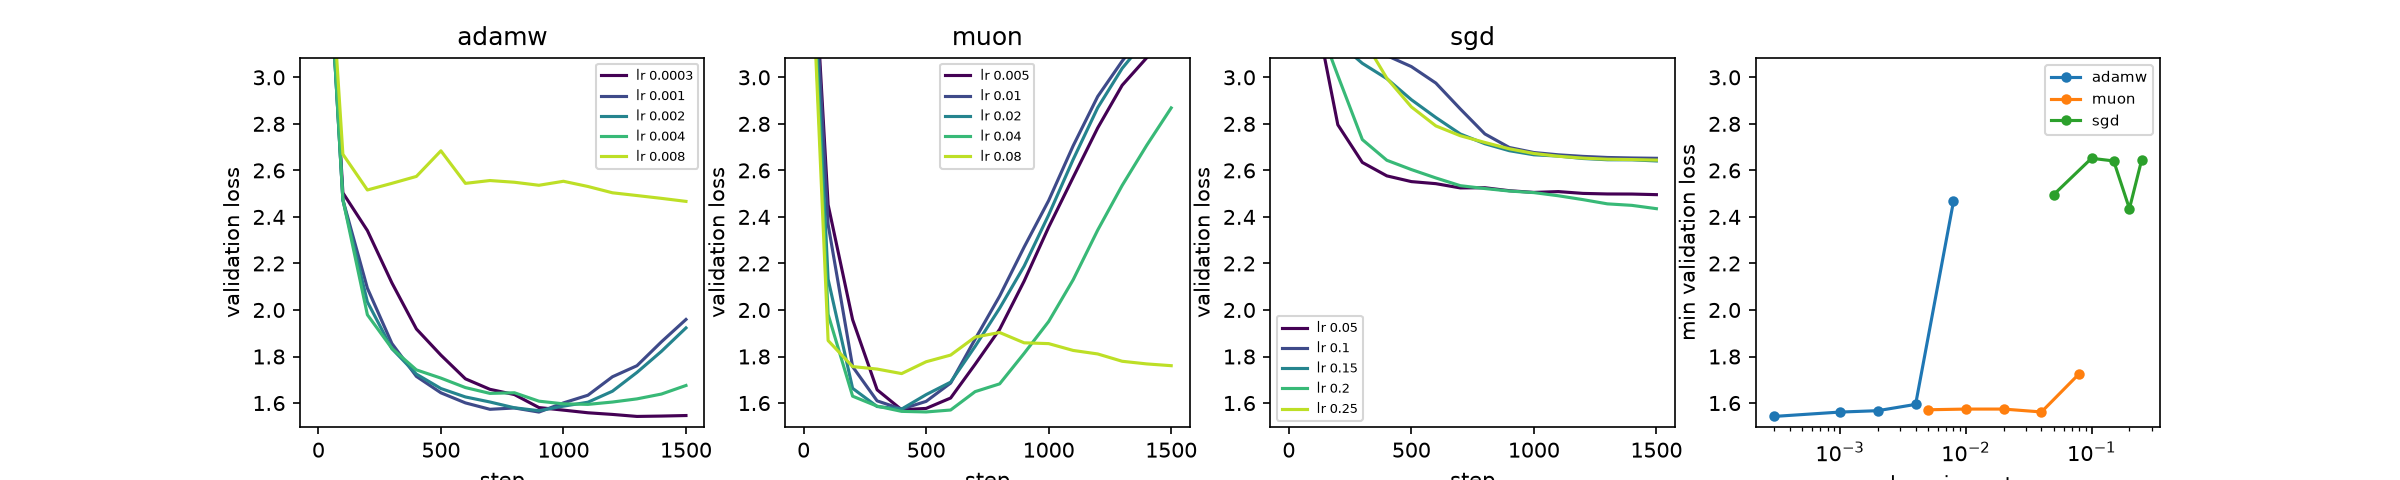
\includegraphics[width=\linewidth]{figures/sweep_shakespeare.png}\\
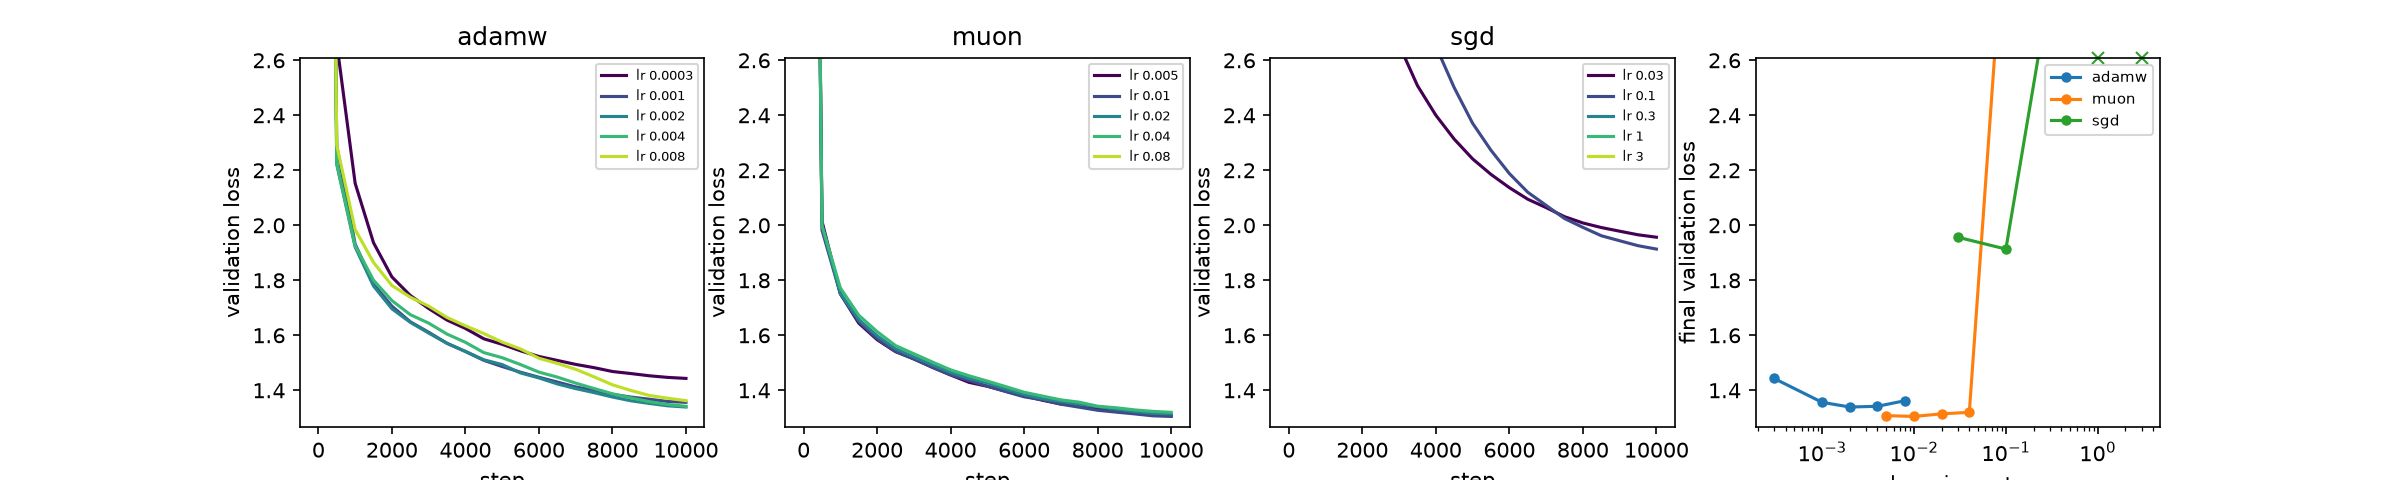
\includegraphics[width=\linewidth]{figures/sweep_ts10m.png}\\
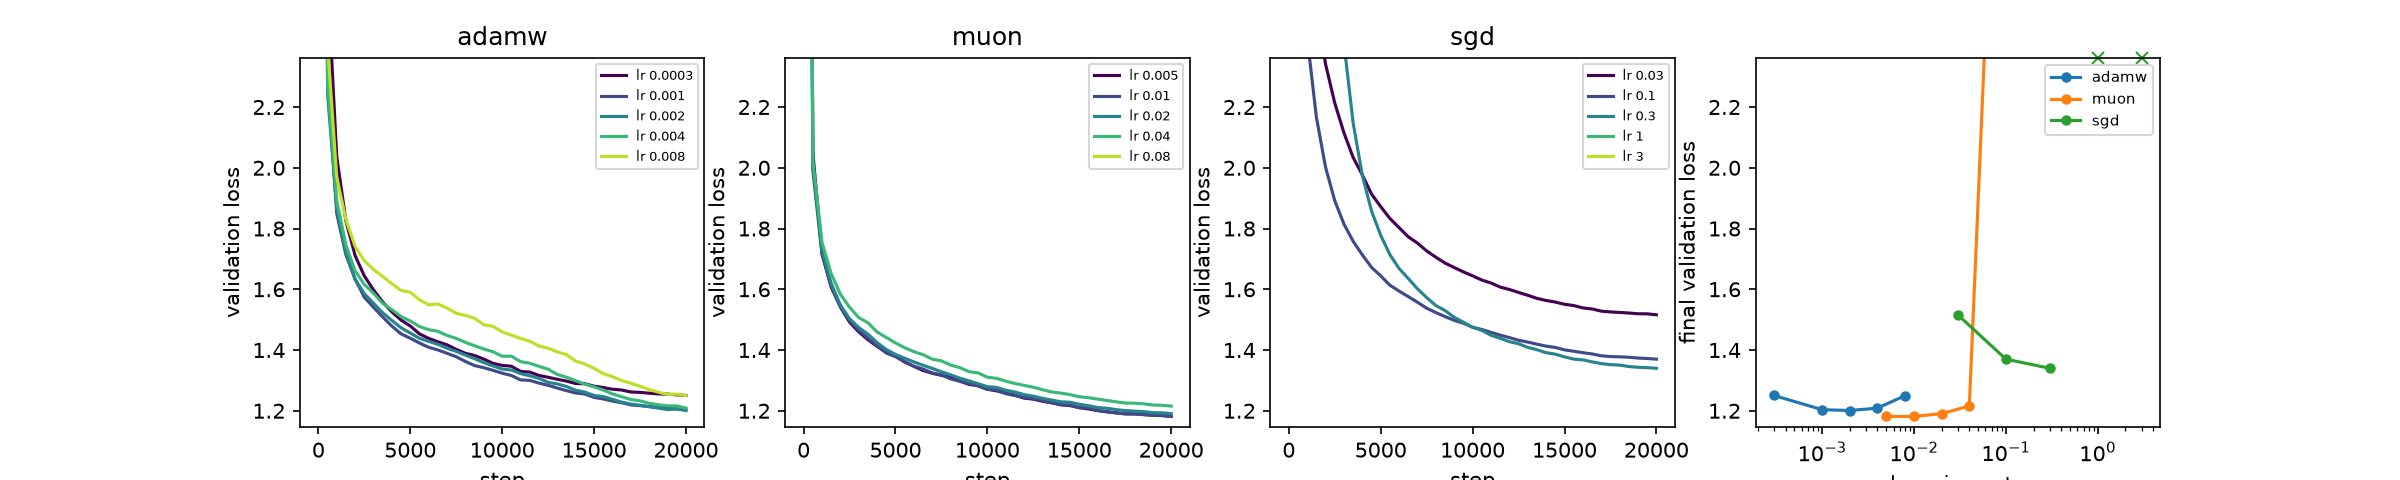
\includegraphics[width=\linewidth]{figures/sweep_ts30m.png}
\caption{Learning-rate sweeps on Shakespeare (top), TinyStories-10M and TinyStories-30M (bottom), data order 0.
One panel per optimizer with the validation loss of each rate against step, and a last panel with the minimum
(Shakespeare) or final (TinyStories) validation loss against the learning rate; $\times$ marks runs that
diverged. Curves above the plotted range are cut.}
\label{fig:sweep}
\end{figure}

\begin{figure}[ht]
\centering
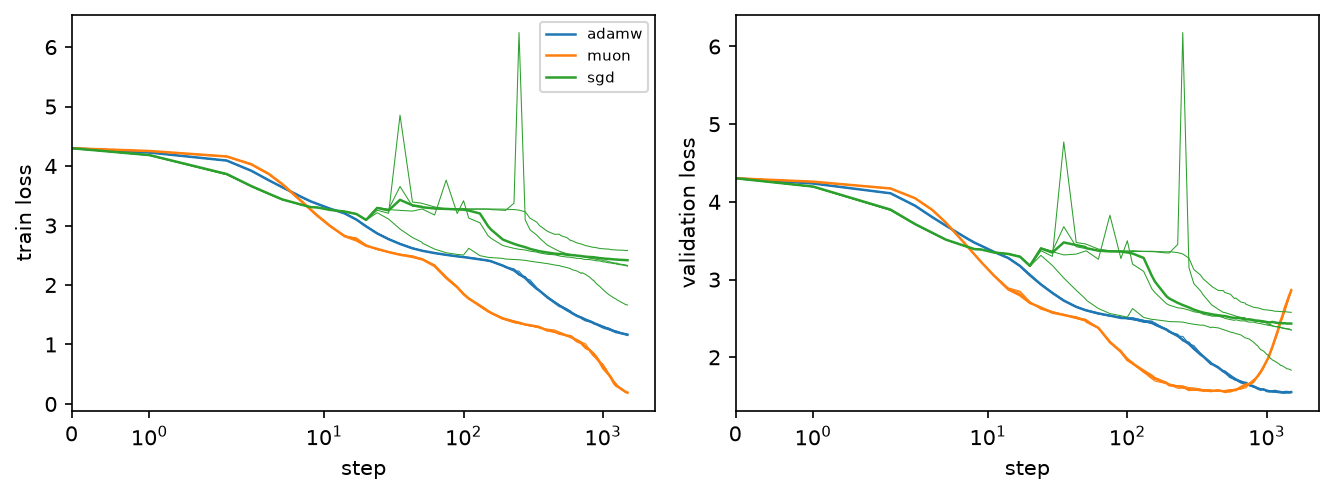
\includegraphics[width=0.49\linewidth]{figures/shakespeare/losses.png}\hfill
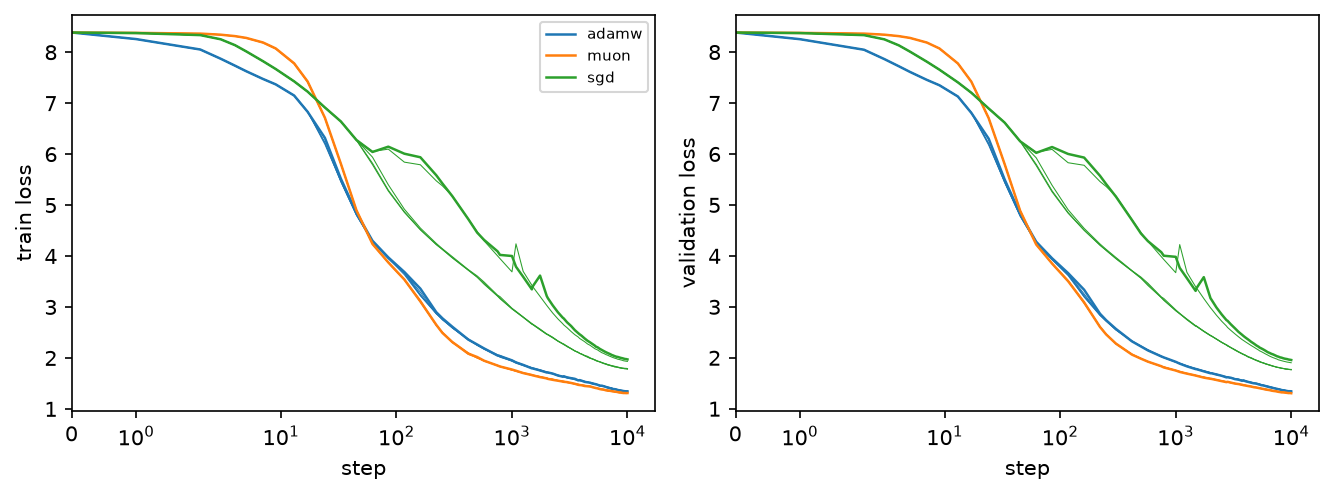
\includegraphics[width=0.49\linewidth]{figures/ts10m/losses.png}\\
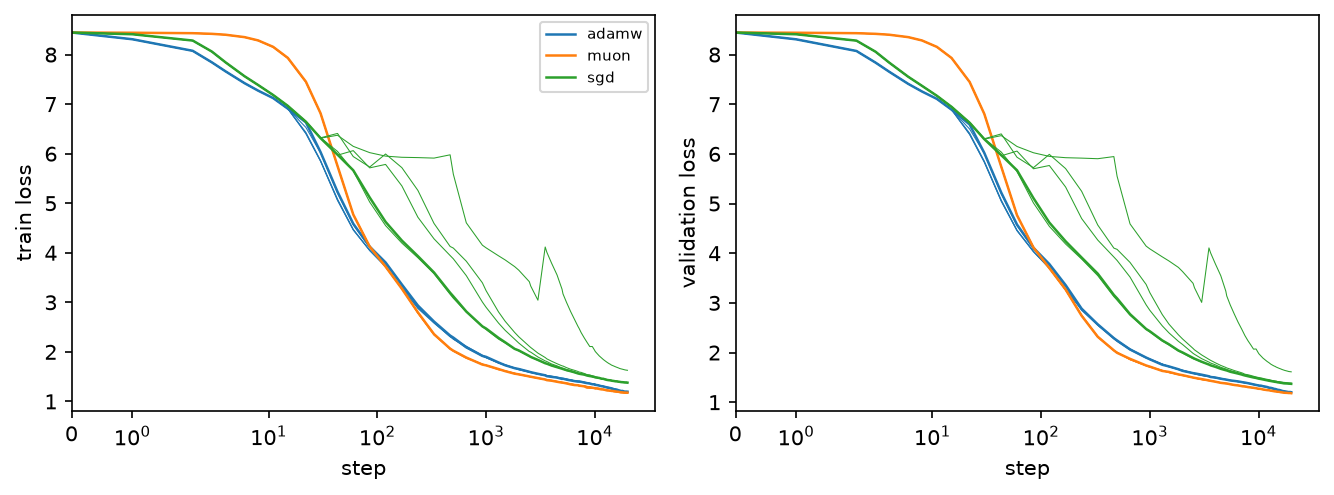
\includegraphics[width=0.49\linewidth]{figures/ts30m/losses.png}
\caption{Training-probe and validation loss of the main runs against step: Shakespeare (top left),
TinyStories-10M (top right), TinyStories-30M (bottom). Data order 0 thick, orders 1--4 thin.}
\label{fig:losses}
\end{figure}

\begin{figure}[ht]
\centering
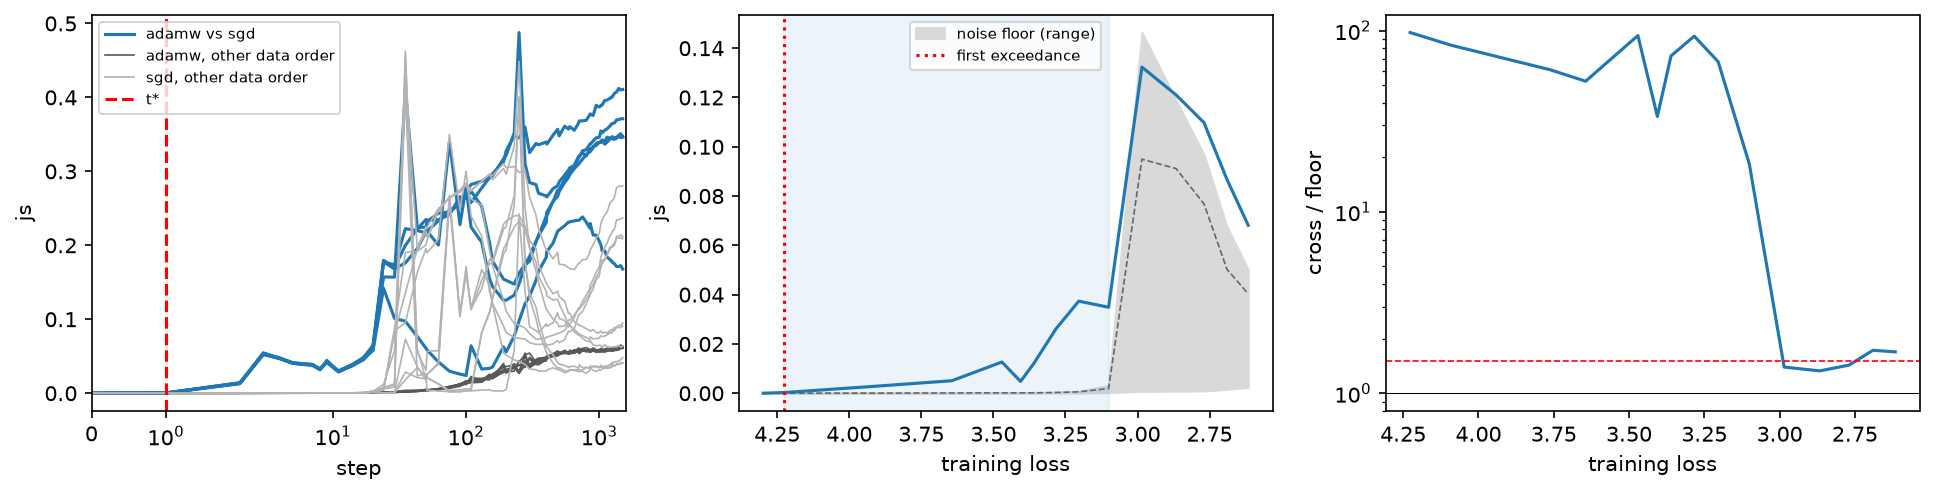
\includegraphics[width=\linewidth]{figures/shakespeare/divergence_adamw_sgd.png}\\
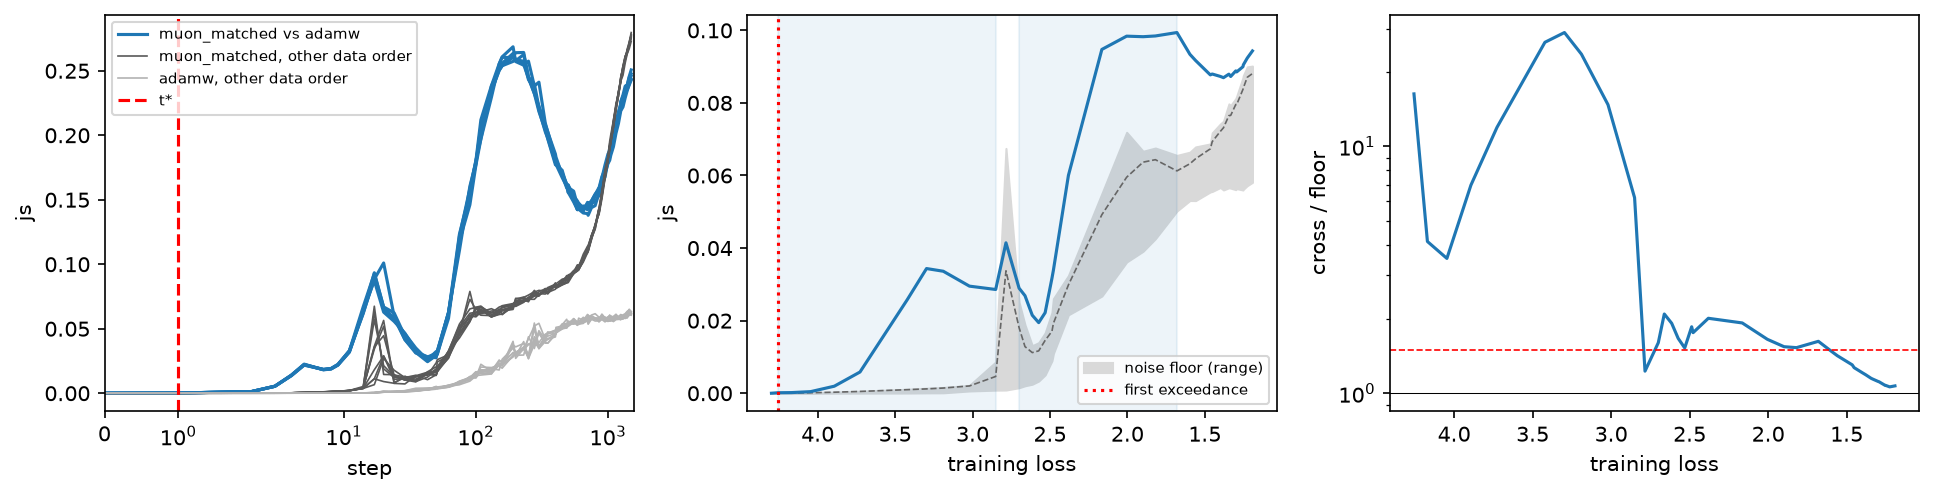
\includegraphics[width=\linewidth]{figures/shakespeare/divergence_matched_adamw.png}\\
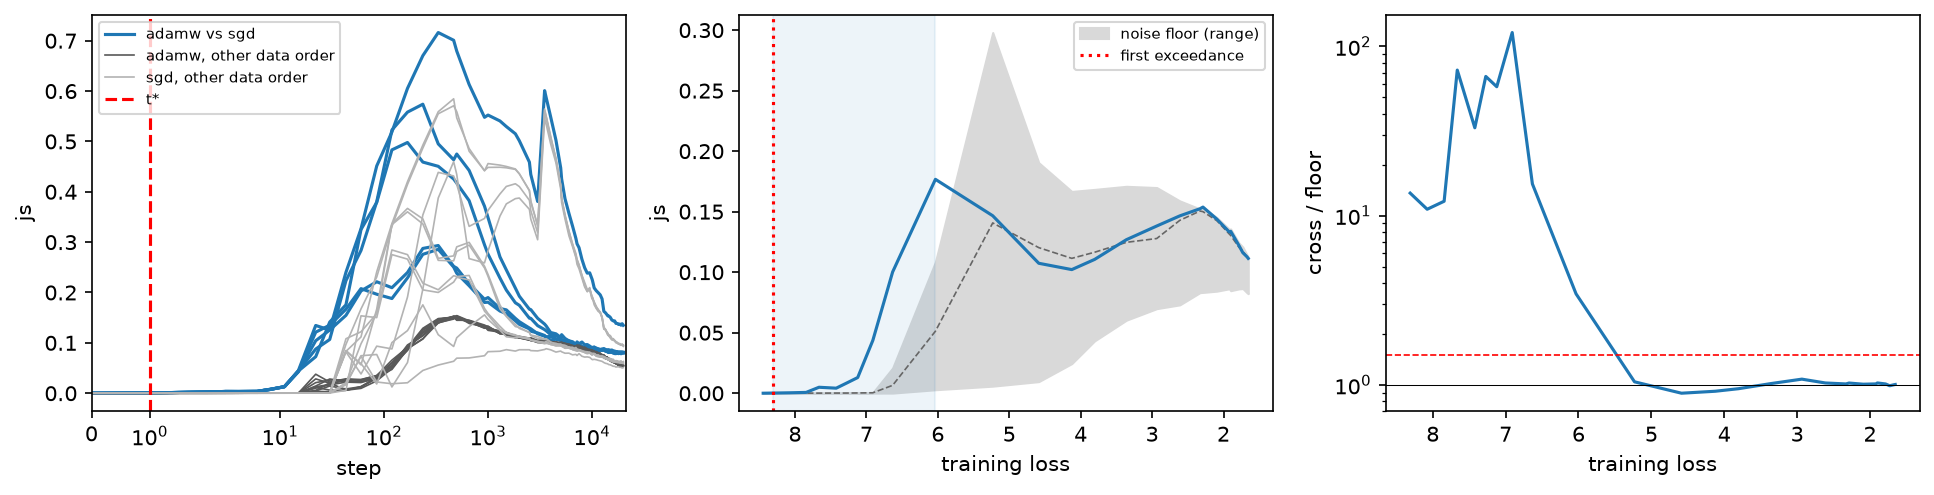
\includegraphics[width=\linewidth]{figures/ts30m/divergence_adamw_sgd.png}\\
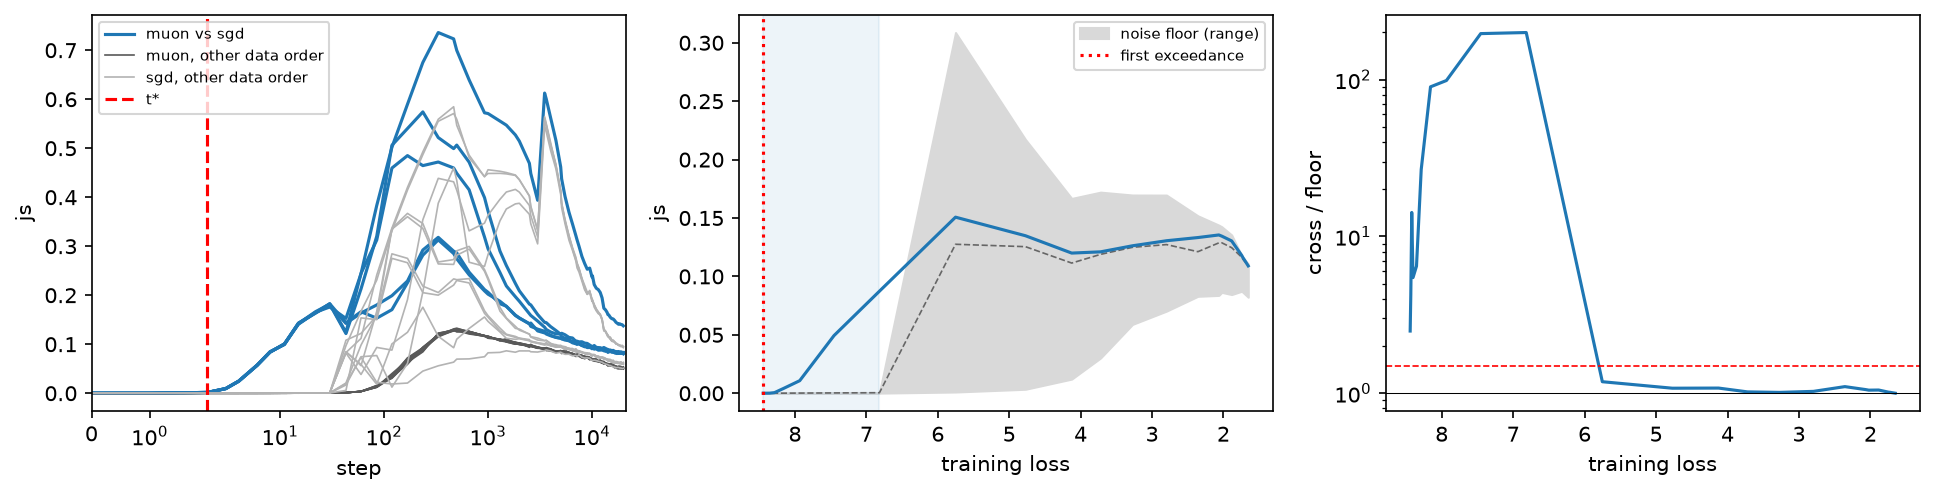
\includegraphics[width=\linewidth]{figures/ts30m/divergence_muon_sgd.png}
\caption{Divergence figures as in \cref{fig:divergence}. Rows: Shakespeare AdamW--SGD; Shakespeare matched
Muon--AdamW (control); TinyStories-30M AdamW--SGD; TinyStories-30M Muon--SGD.}
\label{fig:app-divergence}
\end{figure}

\begin{figure}[ht]
\centering
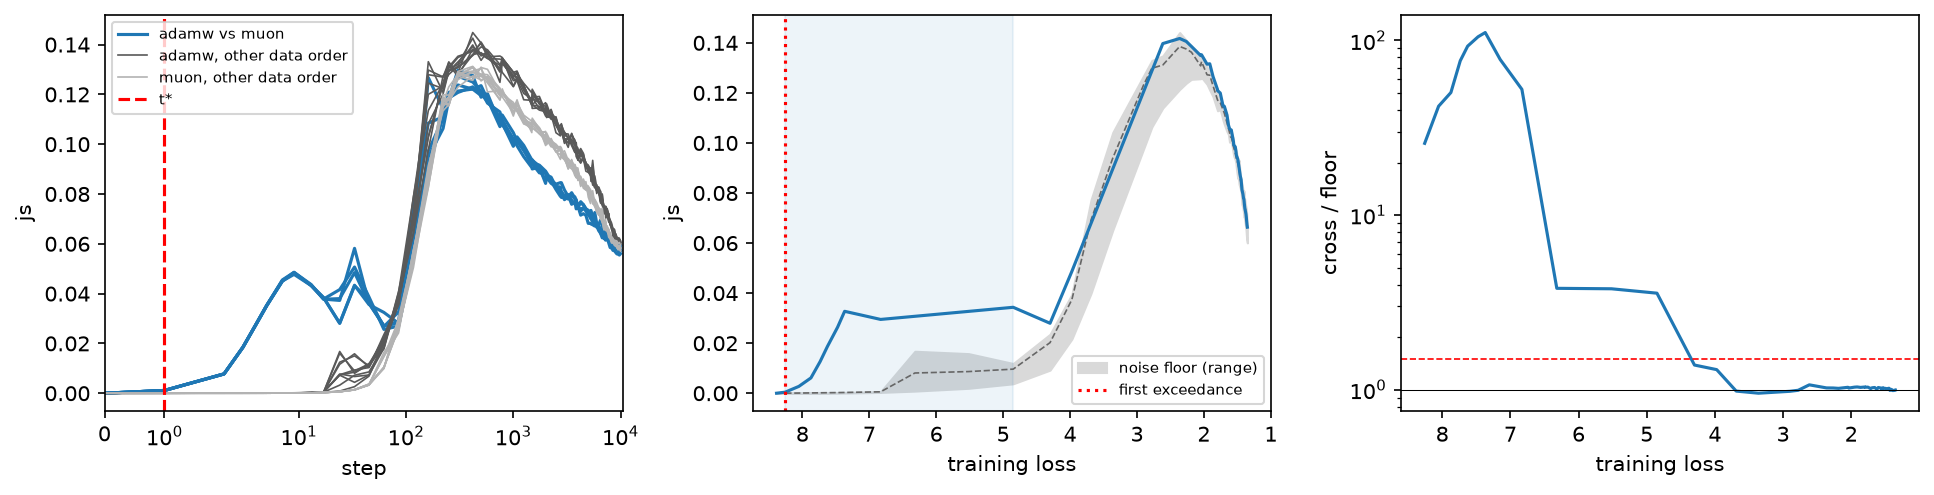
\includegraphics[width=\linewidth]{figures/ts10m/divergence_adamw_muon.png}\\
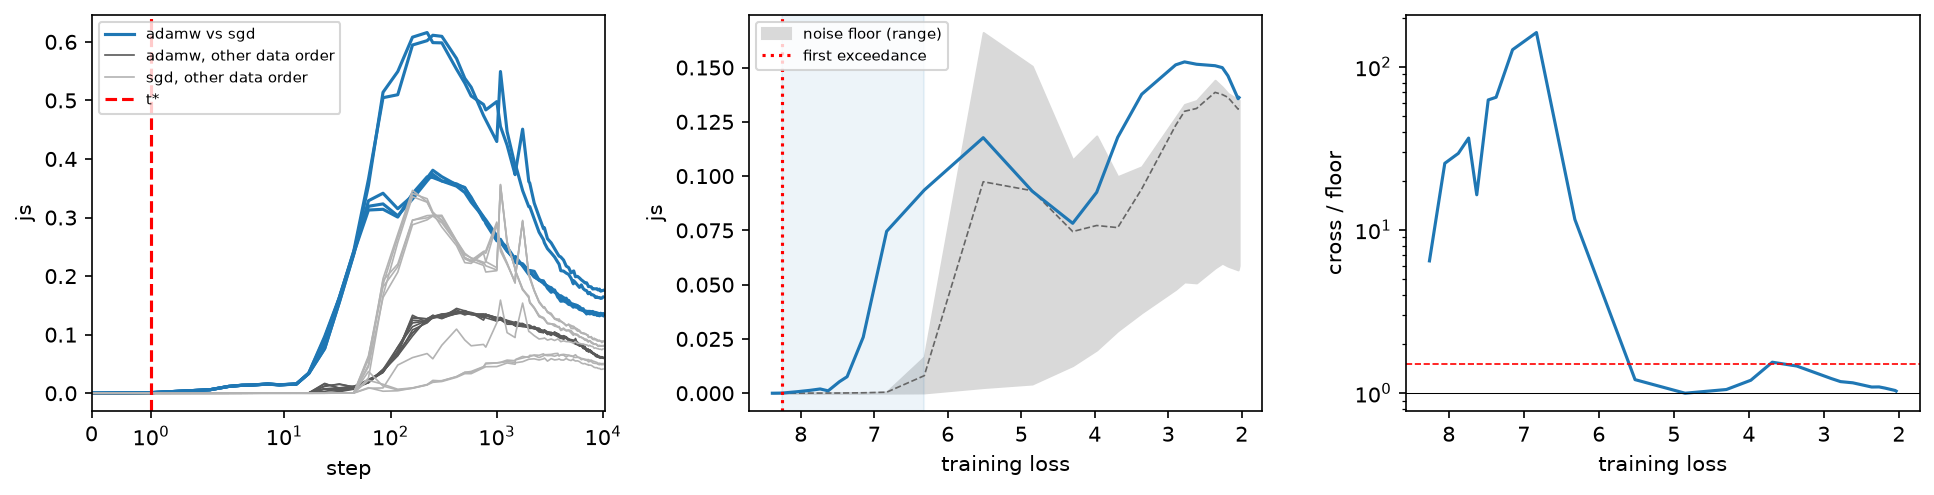
\includegraphics[width=\linewidth]{figures/ts10m/divergence_adamw_sgd.png}\\
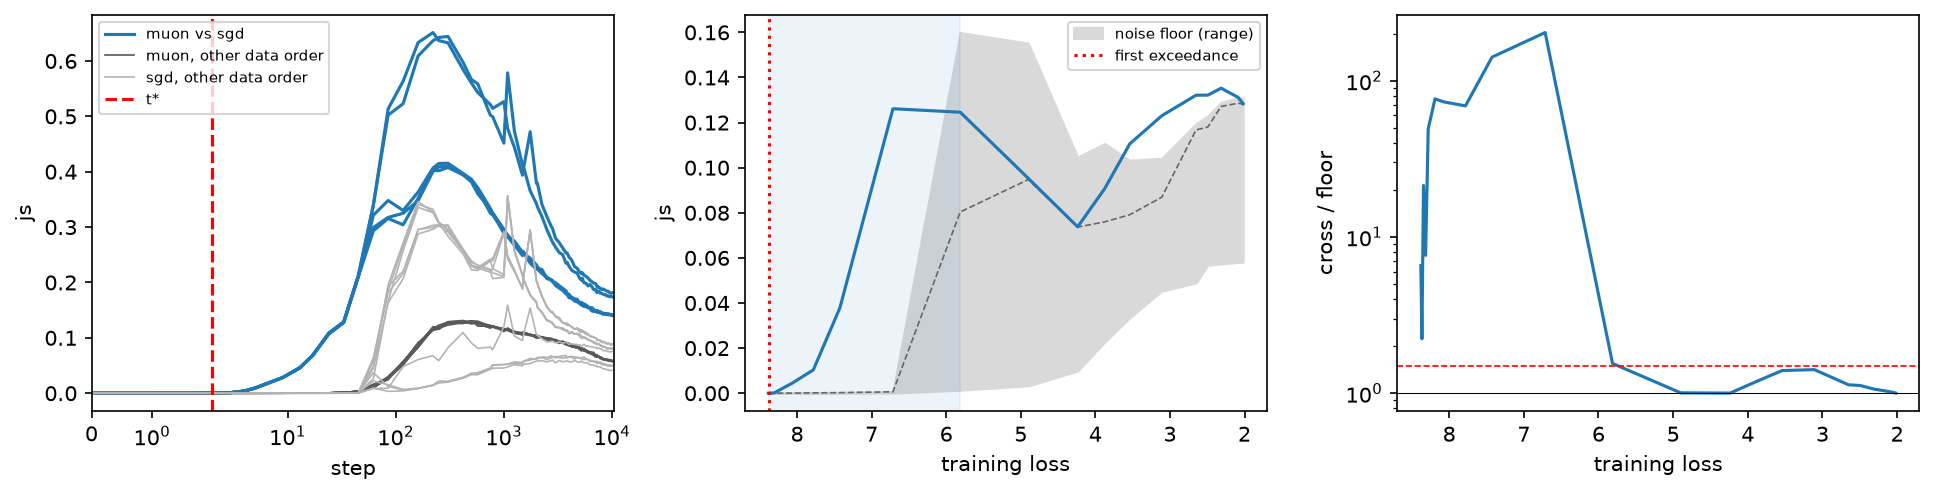
\includegraphics[width=\linewidth]{figures/ts10m/divergence_muon_sgd.png}
\caption{Divergence figures as in \cref{fig:divergence} for TinyStories-10M. Rows: AdamW--Muon, AdamW--SGD,
Muon--SGD.}
\label{fig:app-divergence10}
\end{figure}

\begin{figure}[ht]
\centering
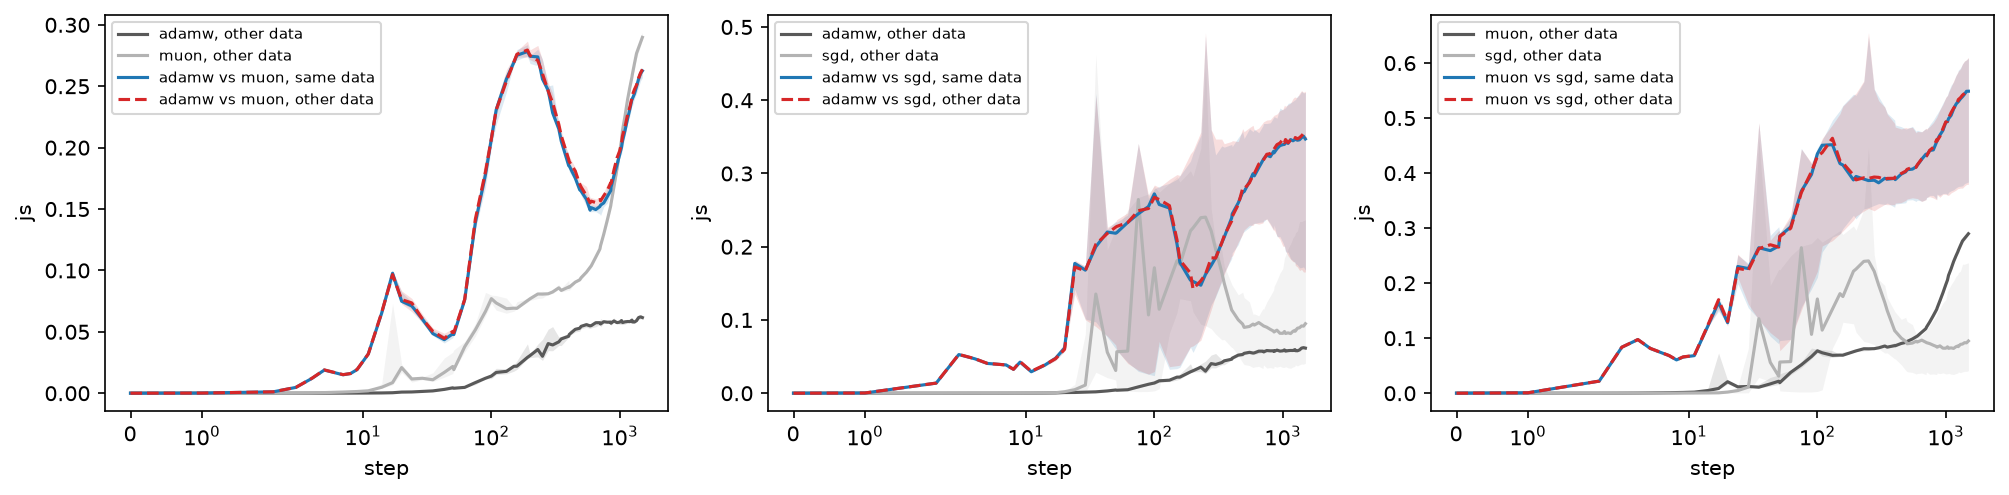
\includegraphics[width=\linewidth]{figures/shakespeare/decompose_js.png}\\[2pt]
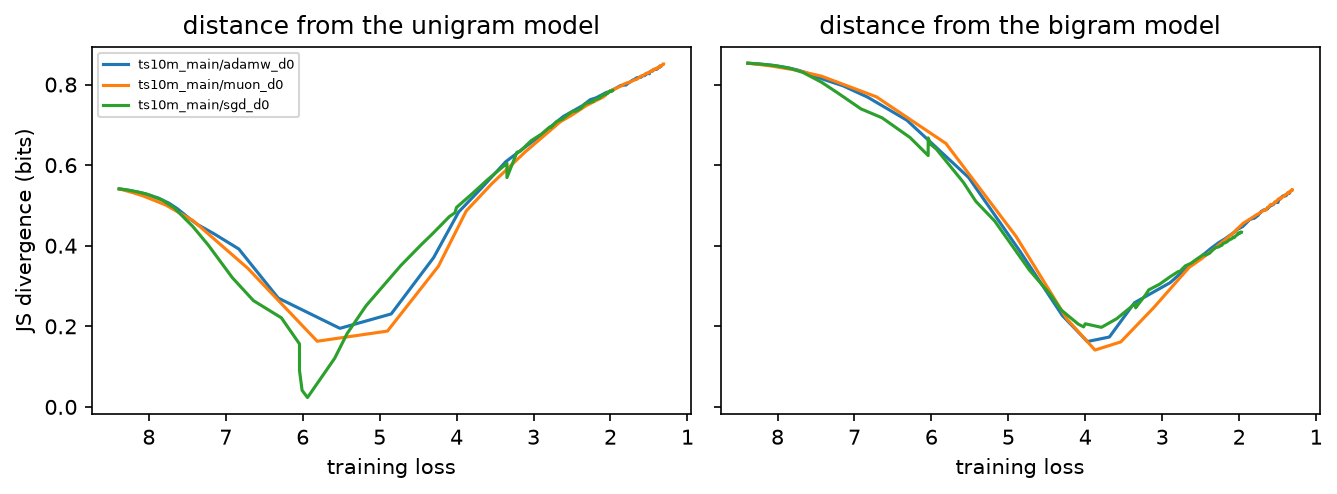
\includegraphics[width=0.49\linewidth]{figures/ts10m/ngram.png}\hfill
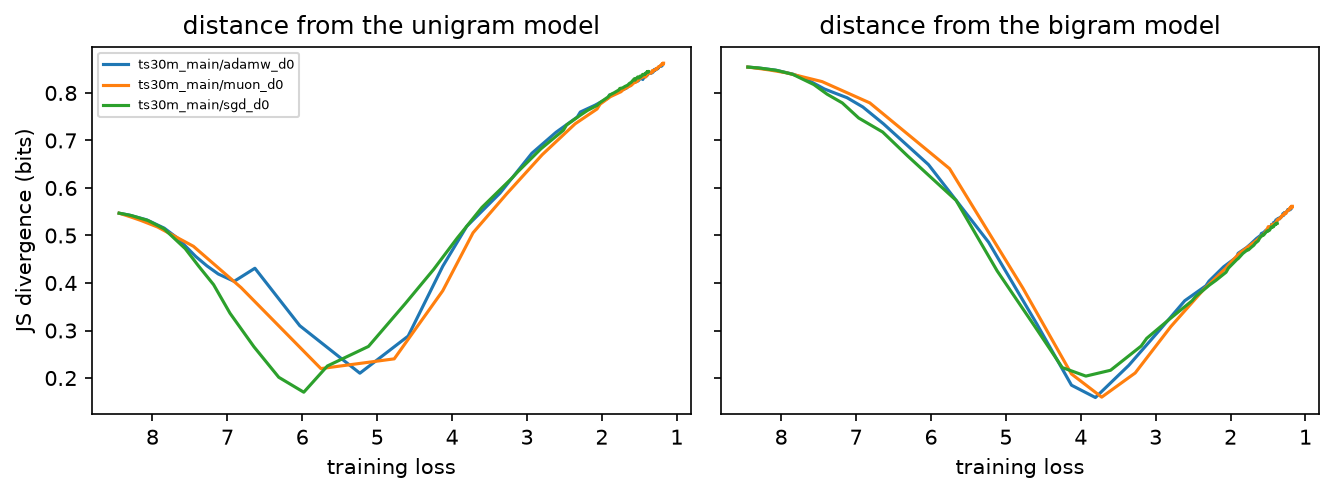
\includegraphics[width=0.49\linewidth]{figures/ts30m/ngram.png}
\caption{Top: optimizer against data order at equal steps on Shakespeare, as in \cref{fig:route} (top), for
the three pairs. Bottom: distance of the $d=0$ runs from the unigram and bigram models on TinyStories-10M
(left) and TinyStories-30M (right), as in \cref{fig:route} (bottom).}
\label{fig:app-route}
\end{figure}

\begin{figure}[ht]
\centering
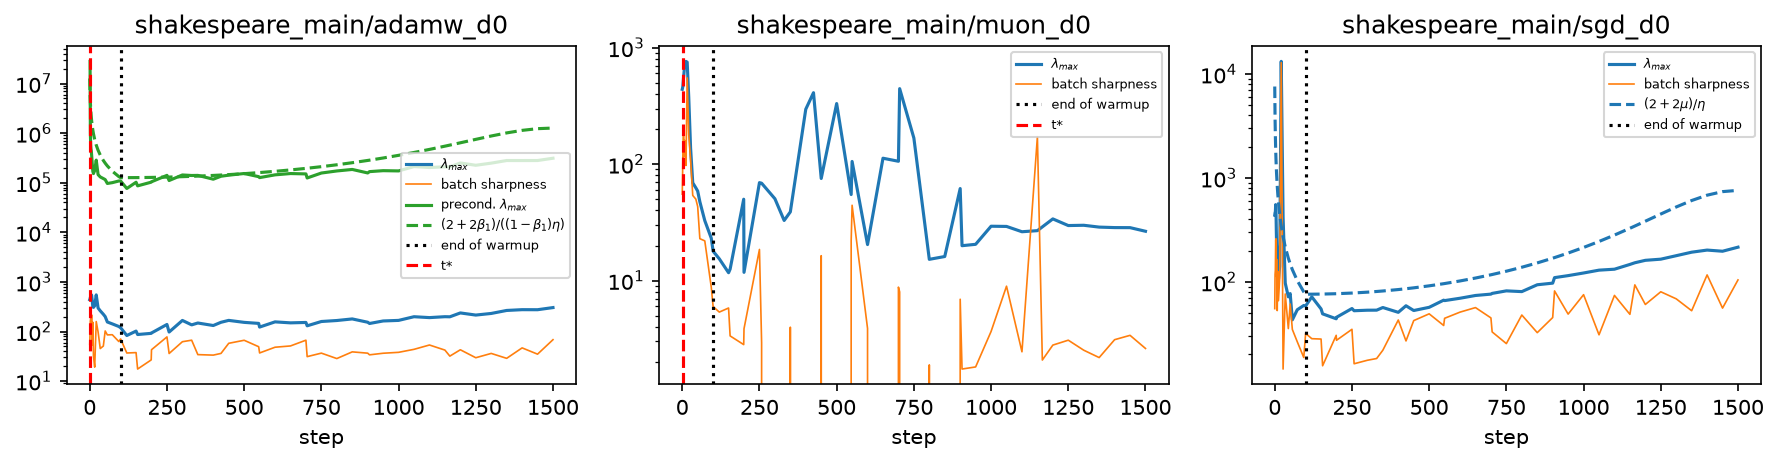
\includegraphics[width=\linewidth]{figures/shakespeare/sharpness.png}\\
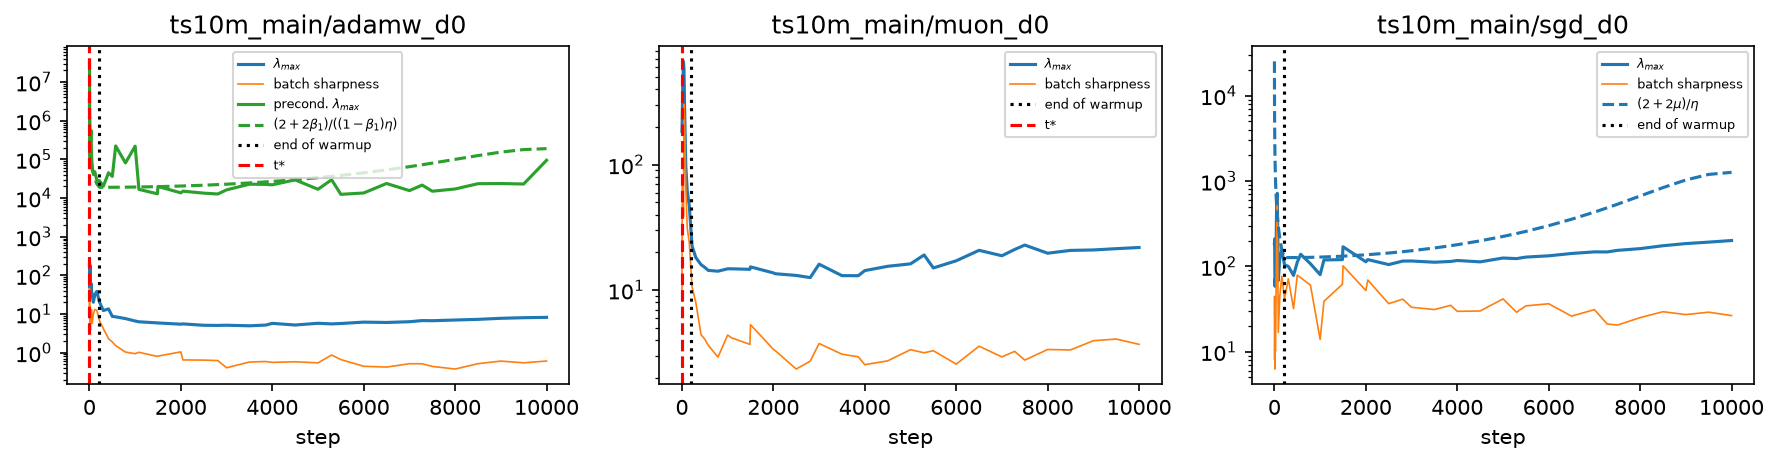
\includegraphics[width=\linewidth]{figures/ts10m/sharpness.png}\\
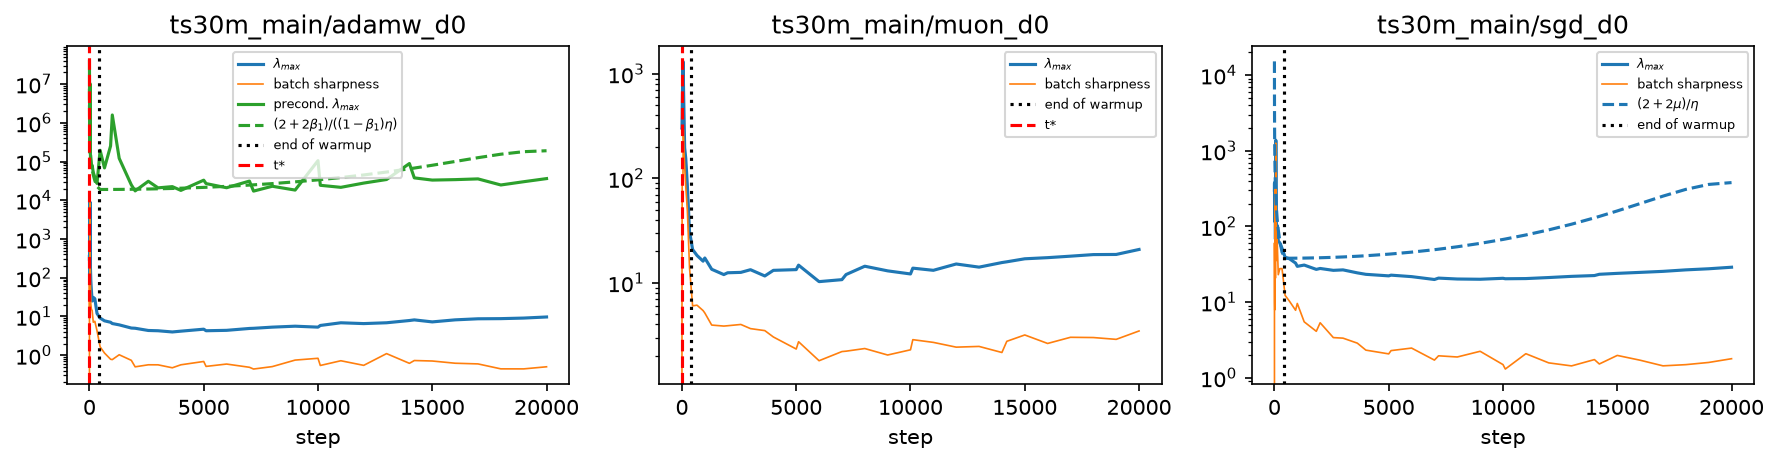
\includegraphics[width=\linewidth]{figures/ts30m/sharpness.png}
\caption{Sharpness of the $d=0$ runs on Shakespeare (top), TinyStories-10M and TinyStories-30M (bottom), log
scale: $\lmax$, batch sharpness, for AdamW the preconditioned sharpness, and the thresholds
$(2+2\mu)/\eta_s$ (SGD) and $(2+2\beta_1)/((1-\beta_1)\eta_s)$ (AdamW, dashed); end of warmup dotted, first
exceedance $t^\ast_X$ of the AdamW--Muon pair red dashed.}
\label{fig:app-sharpness}
\end{figure}

\begin{figure}[ht]
\centering
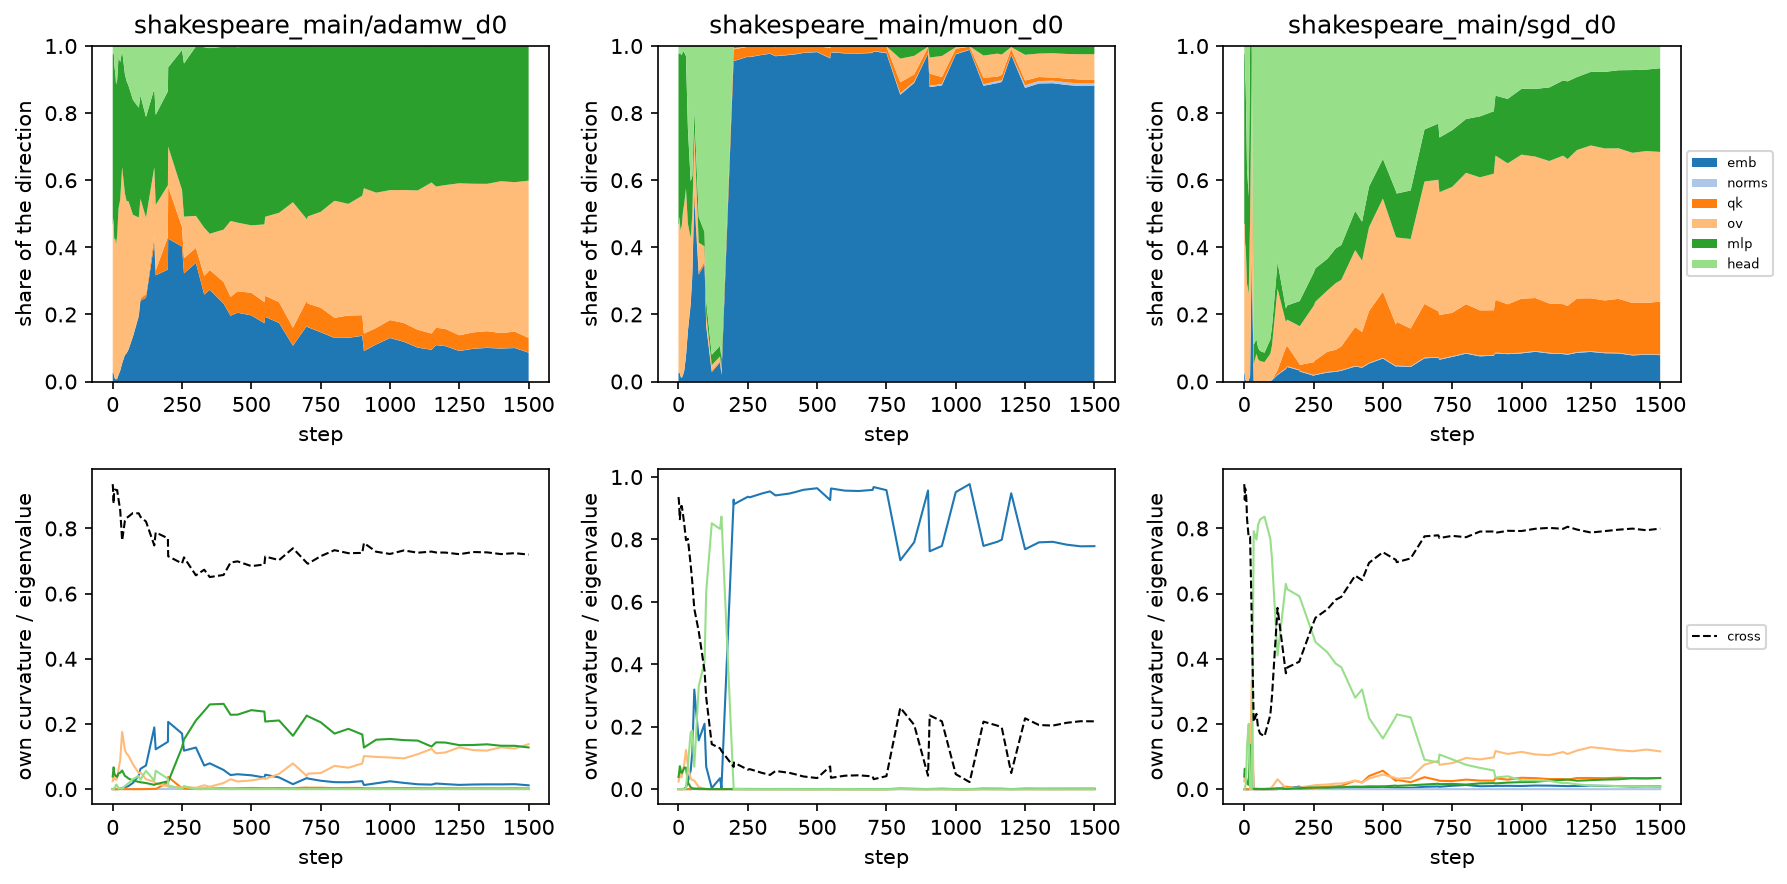
\includegraphics[width=0.78\linewidth]{figures/shakespeare/anatomy.png}\\[2pt]
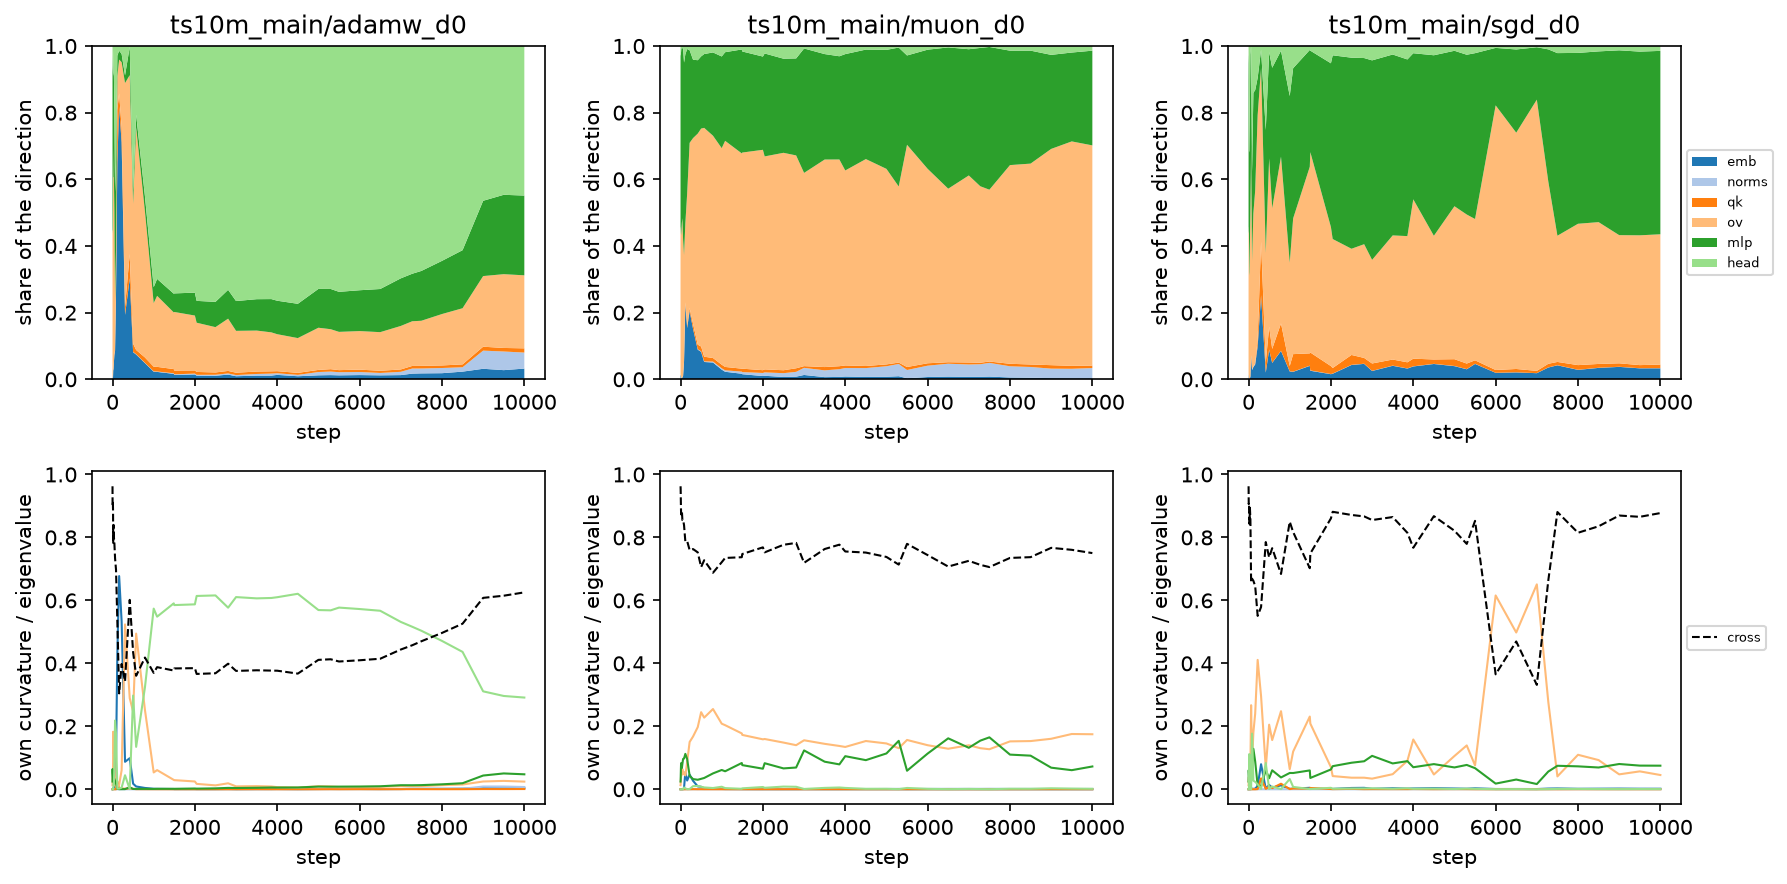
\includegraphics[width=0.78\linewidth]{figures/ts10m/anatomy.png}
\caption{Anatomy of the top Hessian eigenvector as in \cref{fig:anatomy}, on Shakespeare (top two rows) and
TinyStories-10M (bottom two rows).}
\label{fig:app-anatomy}
\end{figure}

\begin{figure}[ht]
\centering
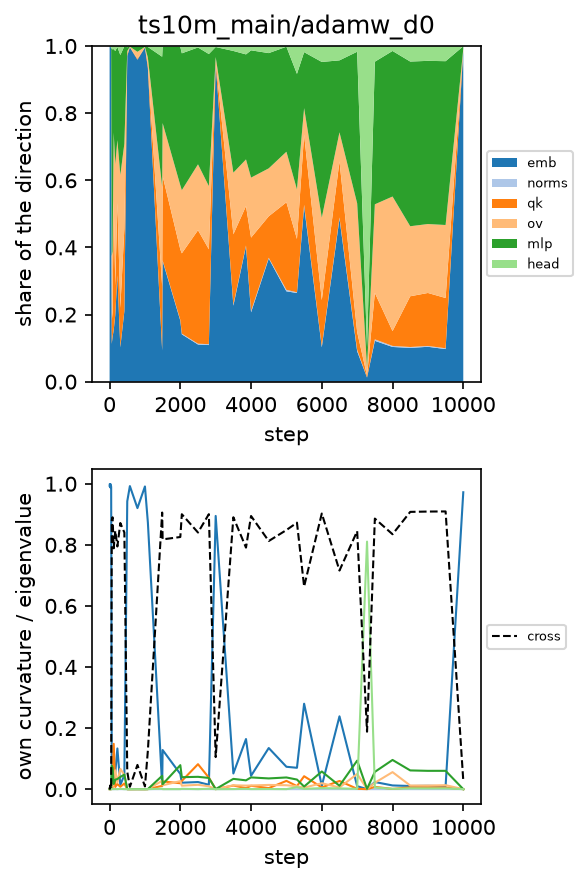
\includegraphics[width=0.32\linewidth]{figures/ts10m/anatomy_precond.png}\qquad
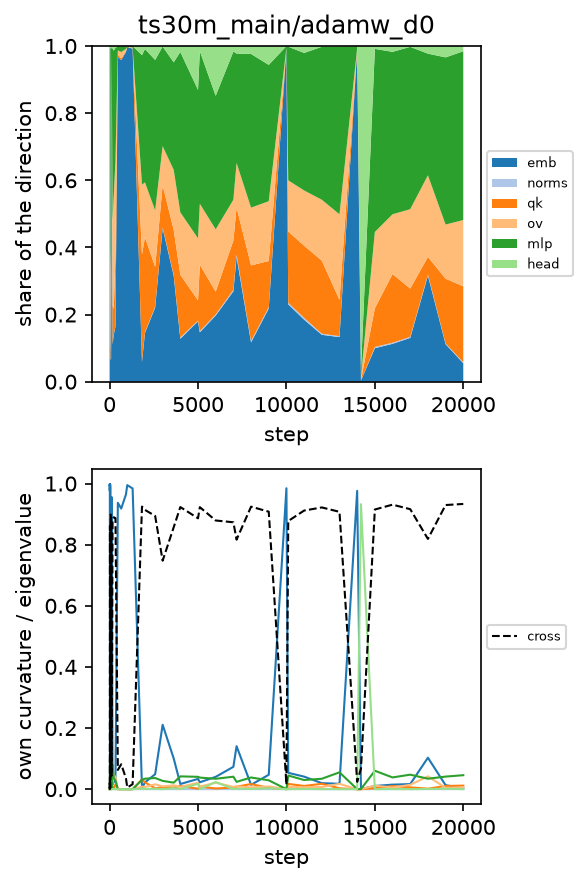
\includegraphics[width=0.32\linewidth]{figures/ts30m/anatomy_precond.png}
\caption{Anatomy of the top eigenvector of AdamW's preconditioned operator $P^{-1/2}HP^{-1/2}$ on
TinyStories-10M (left) and TinyStories-30M (right), as in \cref{fig:anatomy}.}
\label{fig:app-anatomy-precond}
\end{figure}

\begin{figure}[ht]
\centering
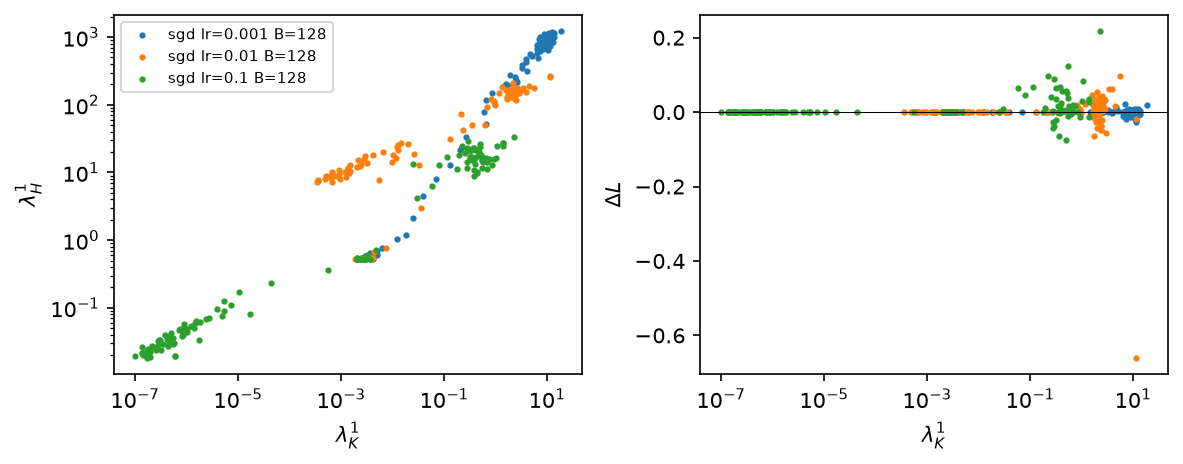
\includegraphics[width=0.6\linewidth]{figures/breakeven/cifar/scatter.png}\\
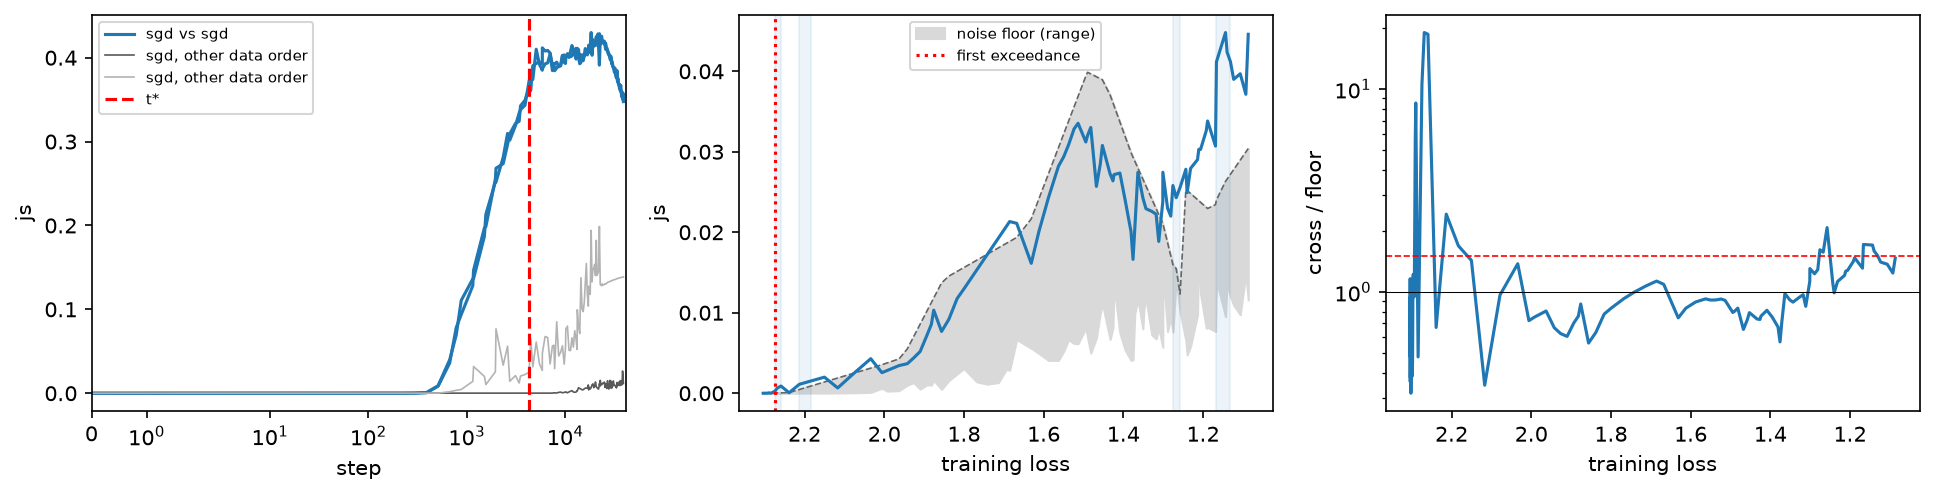
\includegraphics[width=\linewidth]{figures/breakeven/cifar/figures/divergence_0.001_0.01.png}\\
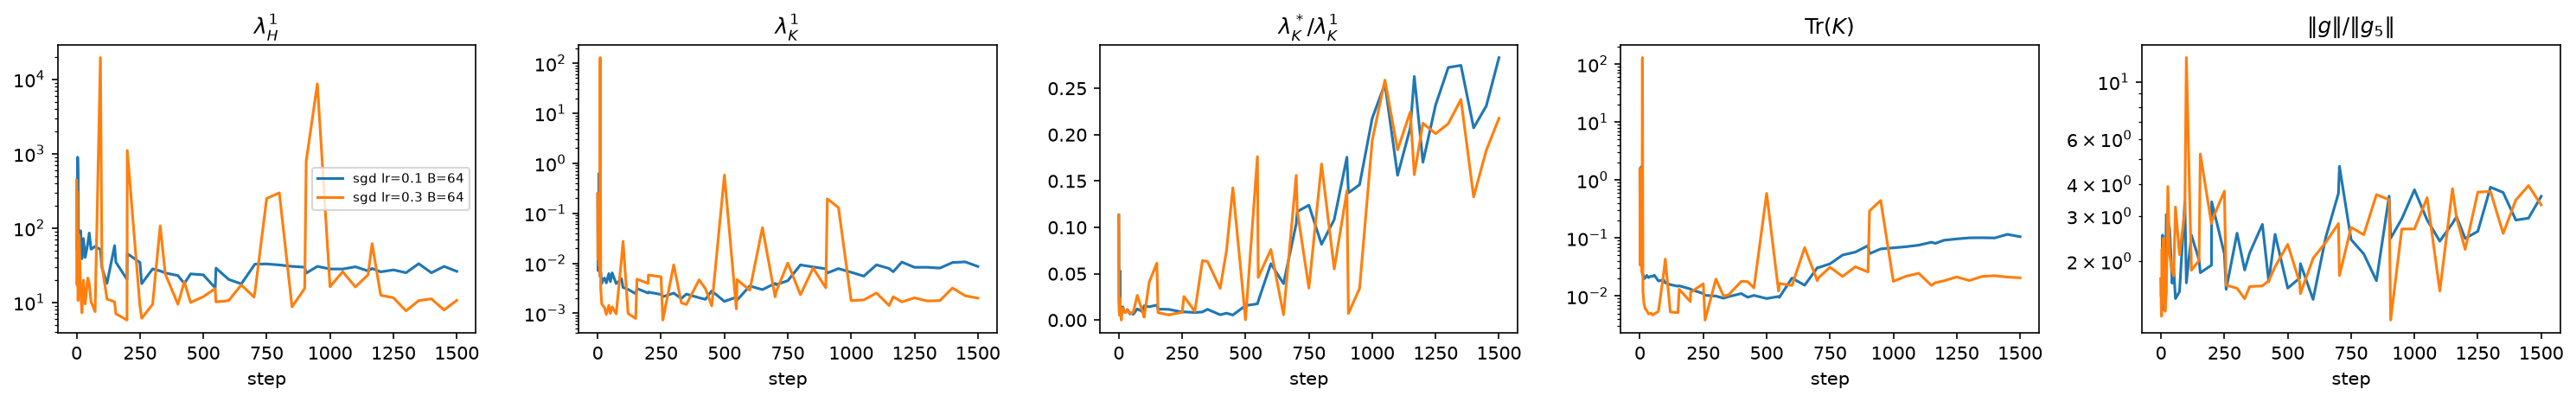
\includegraphics[width=\linewidth]{figures/breakeven/shakespeare/curves.png}\\
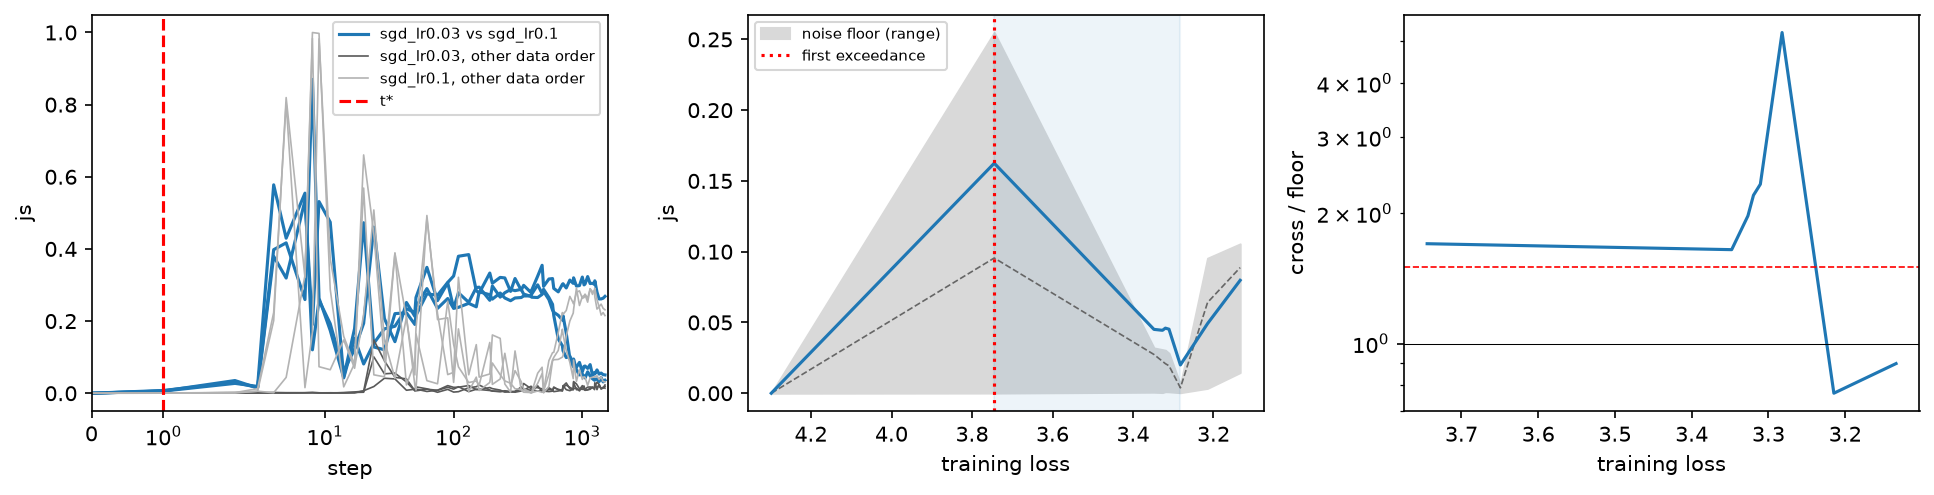
\includegraphics[width=\linewidth]{figures/breakeven/shakespeare/figures/divergence_0.03_0.1.png}
\caption{Break-even analysis, continued. First row: CIFAR-10, $\lambda_H^1$ (left) and $\Delta L$ (right)
against $\lambda_K^1$. Second row: CIFAR-10 divergence figure for $\eta=0.001$ against $0.01$. Third and
fourth rows: Shakespeare with plain SGD at $\eta\in\{0.03,0.1,0.3\}$, the quantities of \cref{fig:breakeven}
(top) and the divergence figure for 0.03 against 0.1.}
\label{fig:app-breakeven}
\end{figure}

\begin{figure}[ht]
\centering
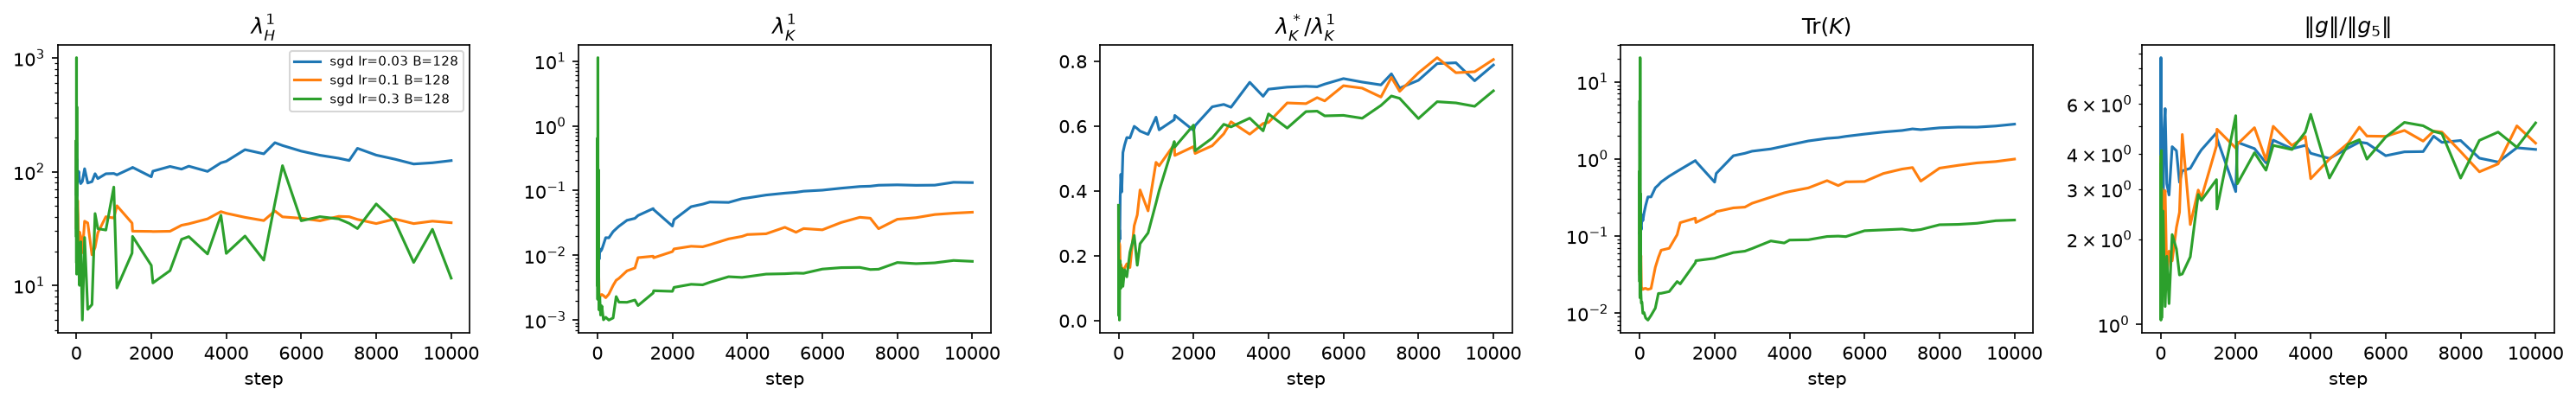
\includegraphics[width=\linewidth]{figures/breakeven/ts10m/curves.png}\\
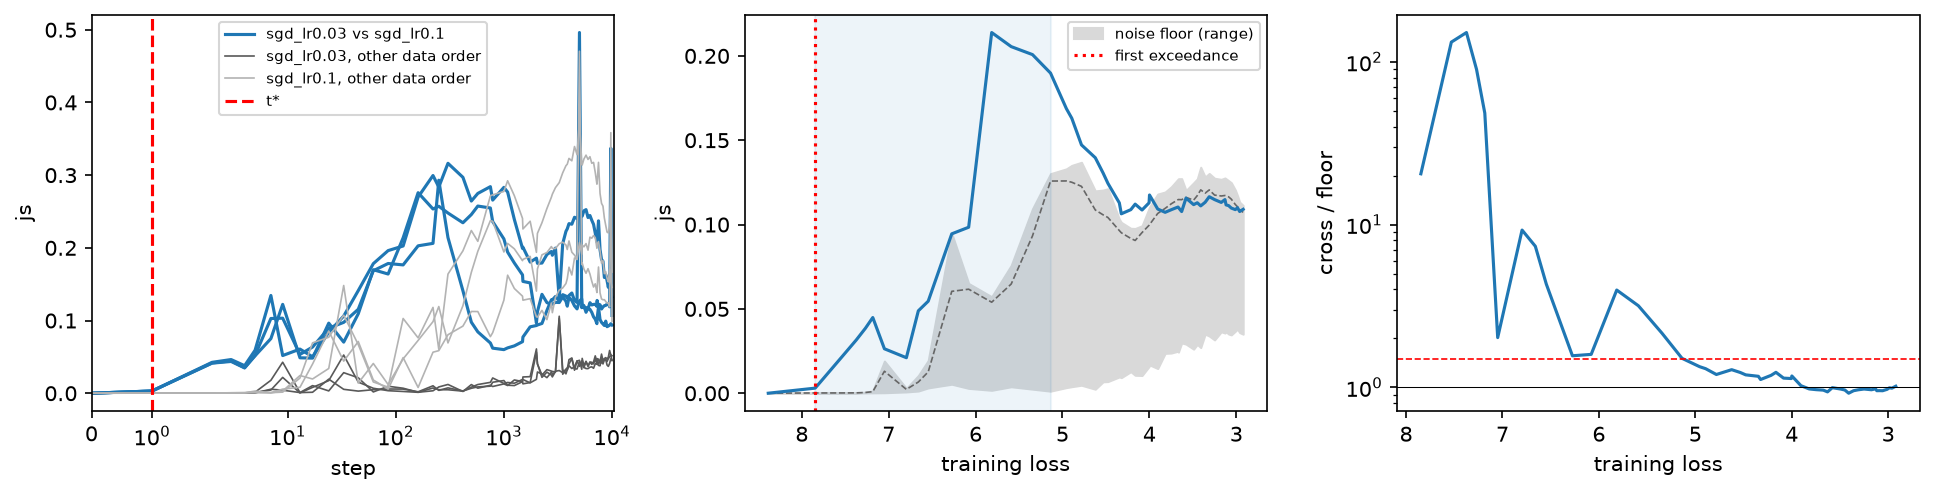
\includegraphics[width=\linewidth]{figures/breakeven/ts10m/figures/divergence_0.03_0.1.png}\\
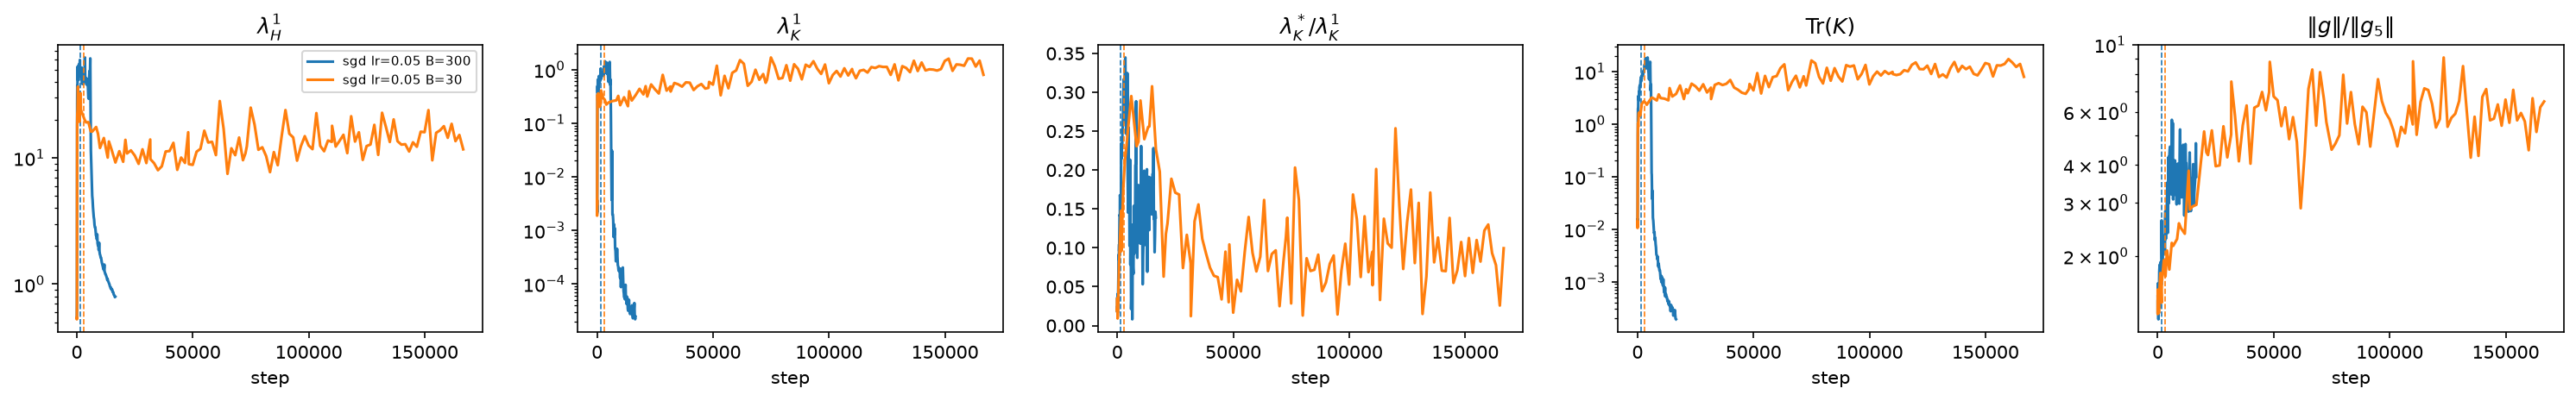
\includegraphics[width=\linewidth]{figures/breakeven/cifar_bs/curves.png}\\
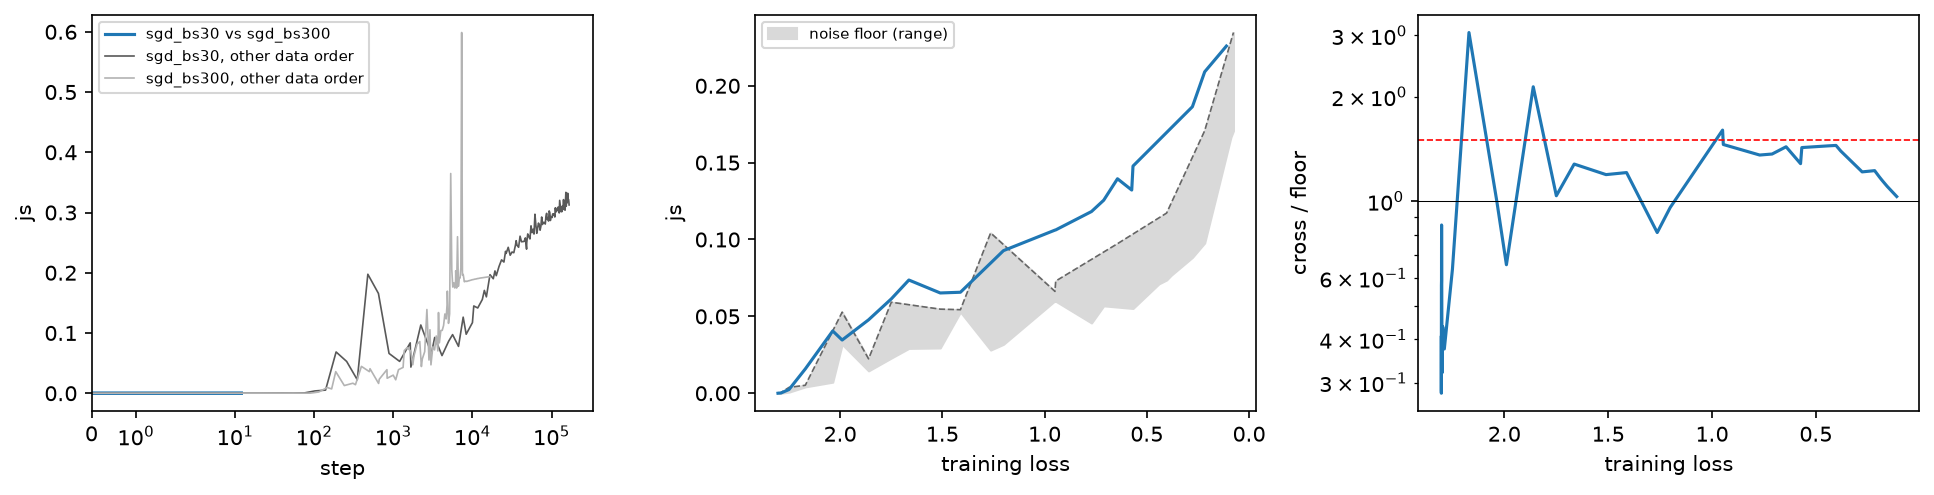
\includegraphics[width=\linewidth]{figures/breakeven/cifar_bs/figures/divergence_bs30_bs300.png}
\caption{Break-even analysis, continued. First two rows: TinyStories-10M with plain SGD at
$\eta\in\{0.03,0.1,0.3\}$, the quantities of \cref{fig:breakeven} and the divergence figure for 0.03 against
0.1. Last two rows: CIFAR-10 at $\eta=0.05$ with batch sizes 30 and 300.}
\label{fig:app-breakeven2}
\end{figure}

\begin{figure}[ht]
\centering
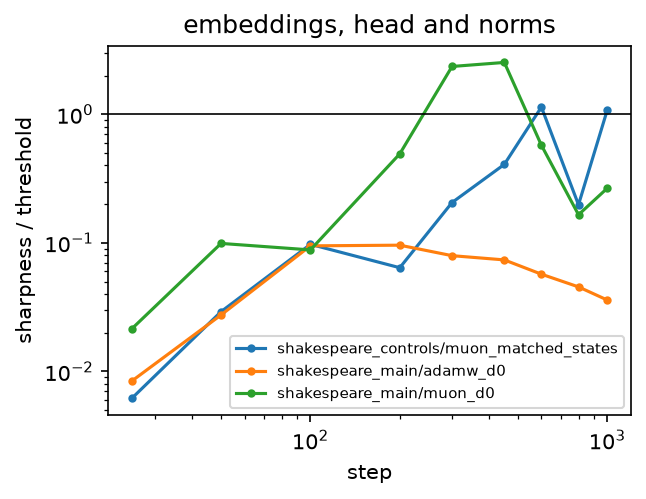
\includegraphics[width=0.45\linewidth]{figures/shakespeare/aux_eos_matched.png}
\caption{Sharpness of the embeddings, head and gains over their stability threshold (\cref{sec:method-aux}) on
Shakespeare, at the fork checkpoints of AdamW, Muon, and Muon with its auxiliary AdamW matched to AdamW
(learning rate $3\cdot10^{-4}$, betas 0.9/0.99, weight decay 0.1).}
\label{fig:app-auxeos}
\end{figure}

\begin{figure}[ht]
\centering
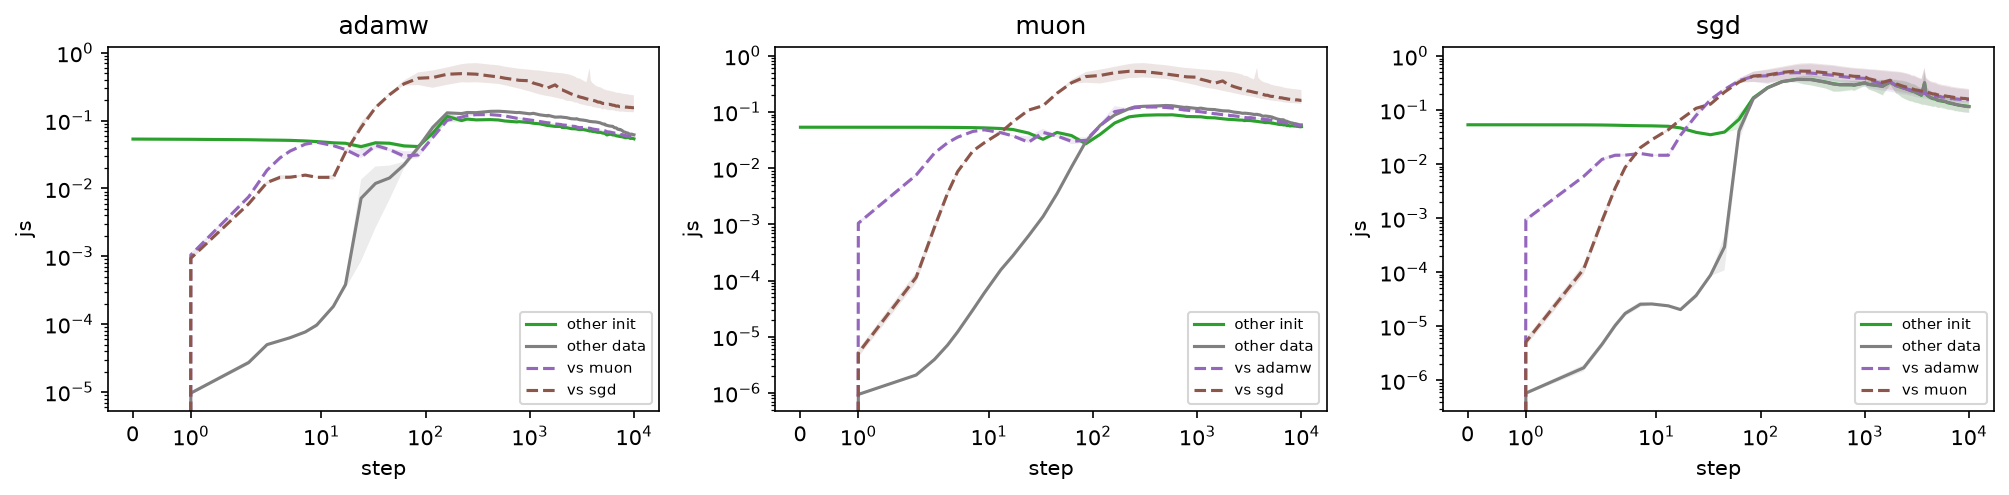
\includegraphics[width=\linewidth]{figures/ts10m/initseed_js.png}
\caption{Second initialization on TinyStories-10M, as in \cref{fig:controls} (top).}
\label{fig:app-initseed}
\end{figure}

\begin{figure}[ht]
\centering
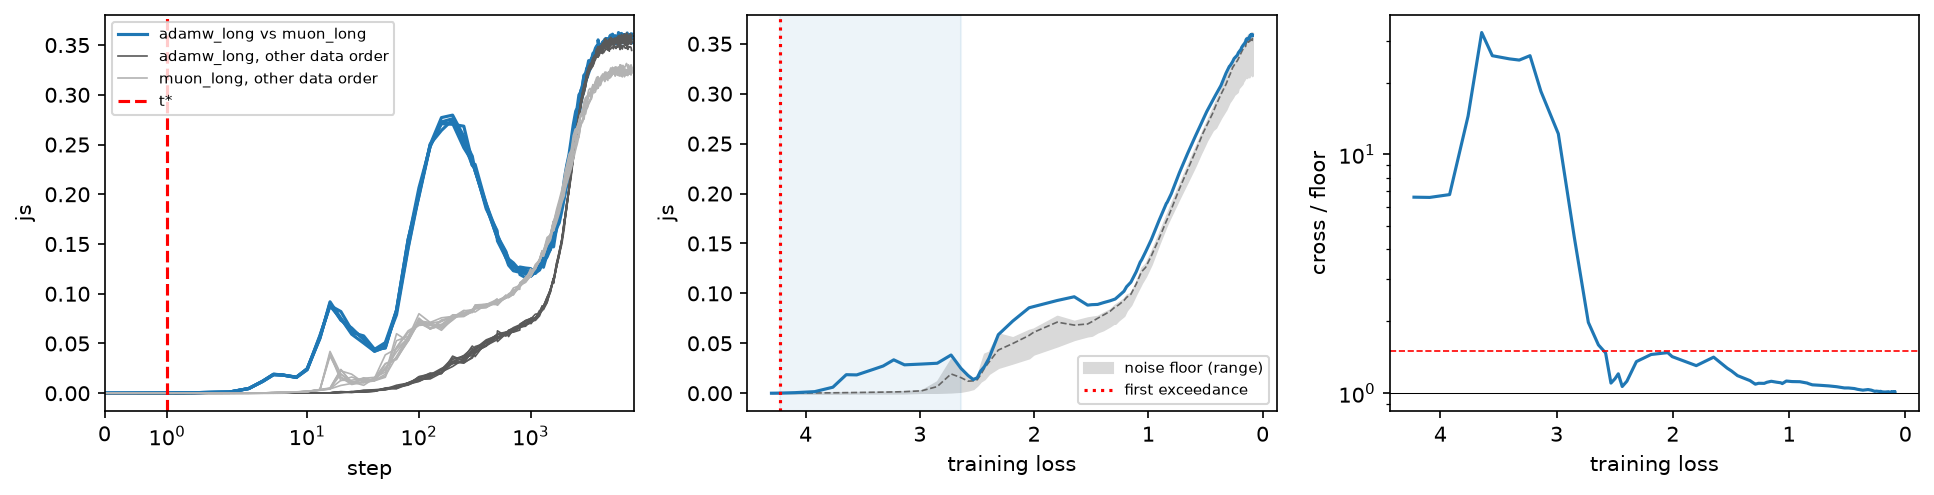
\includegraphics[width=\linewidth]{figures/shakespeare_long/divergence_adamw_muon.png}
\caption{AdamW against Muon on Shakespeare trained for 8000 steps into memorization, as in
\cref{fig:divergence}.}
\label{fig:app-long}
\end{figure}

\begin{figure}[ht]
\centering
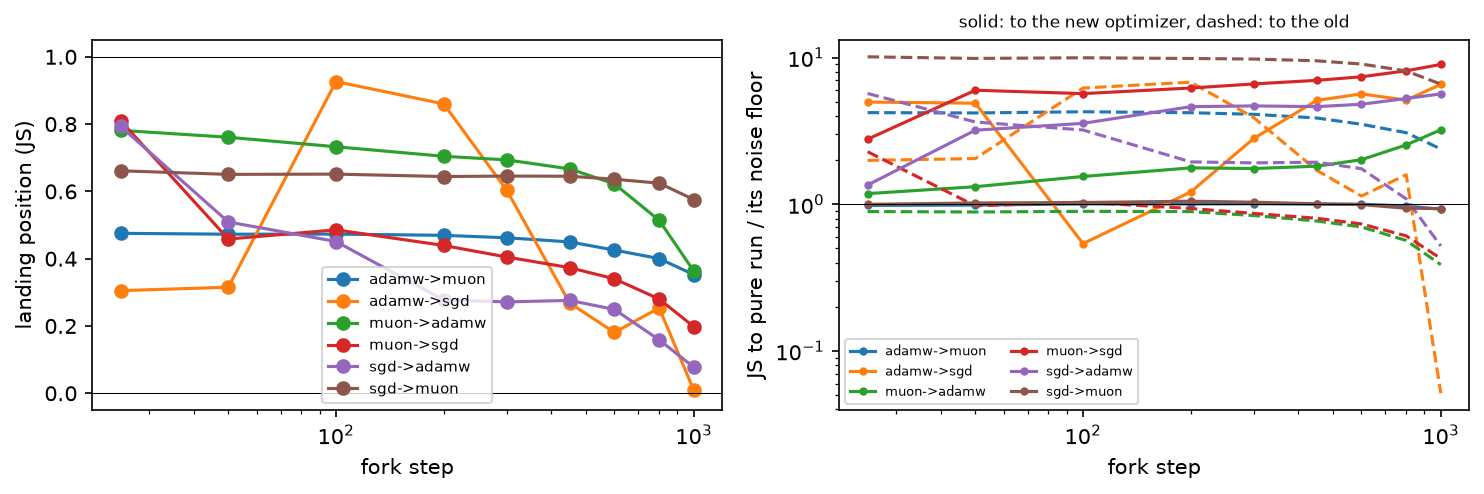
\includegraphics[width=0.75\linewidth]{figures/shakespeare/swap.png}\\[2pt]
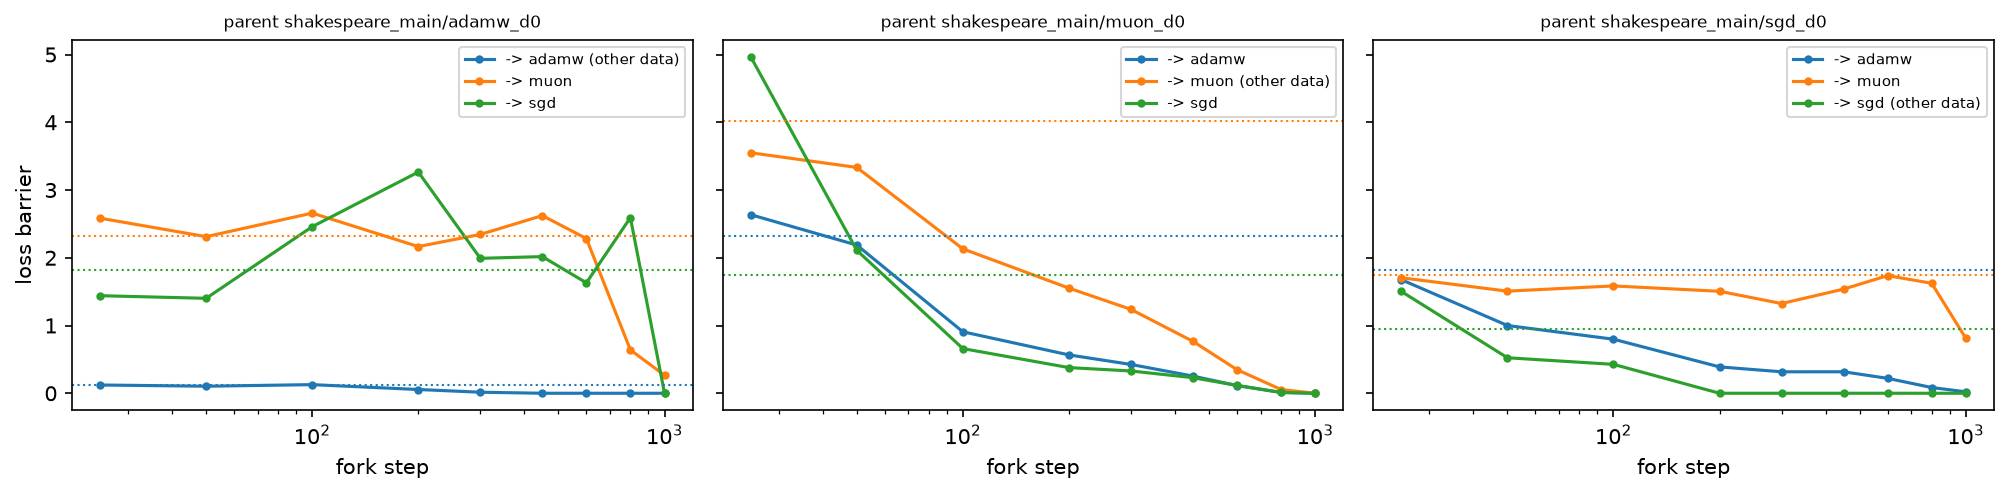
\includegraphics[width=\linewidth]{figures/shakespeare/lmc.png}
\caption{Swaps (top) and mode connectivity (bottom) on Shakespeare, as in \cref{fig:swap}.}
\label{fig:app-swap}
\end{figure}

\begin{figure}[ht]
\centering
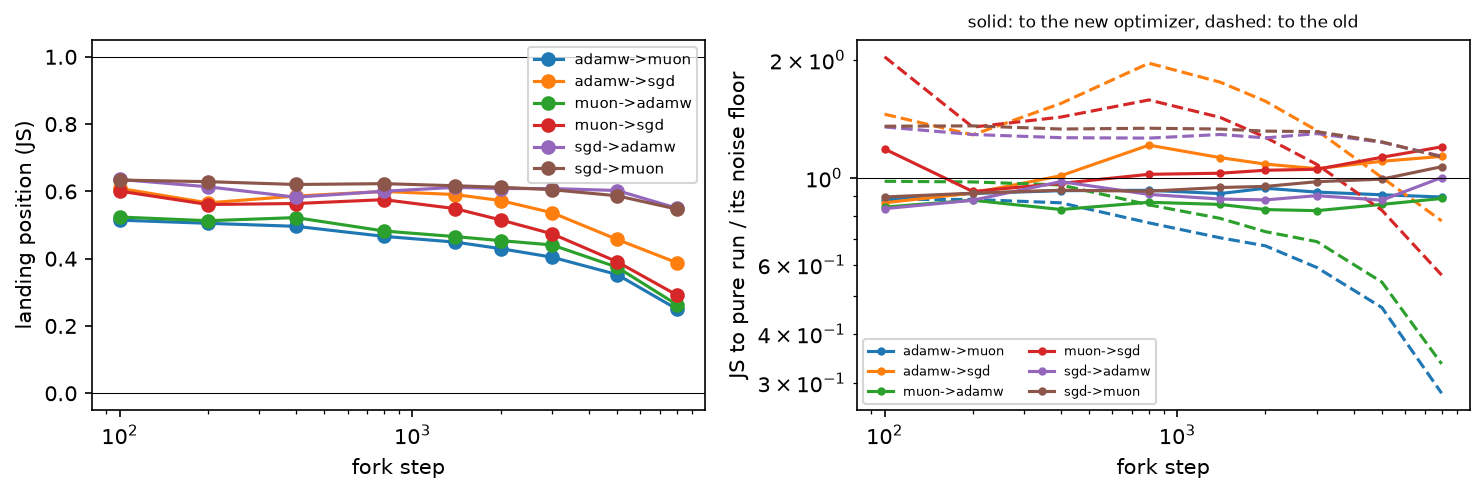
\includegraphics[width=0.75\linewidth]{figures/ts30m/swap.png}\\[2pt]
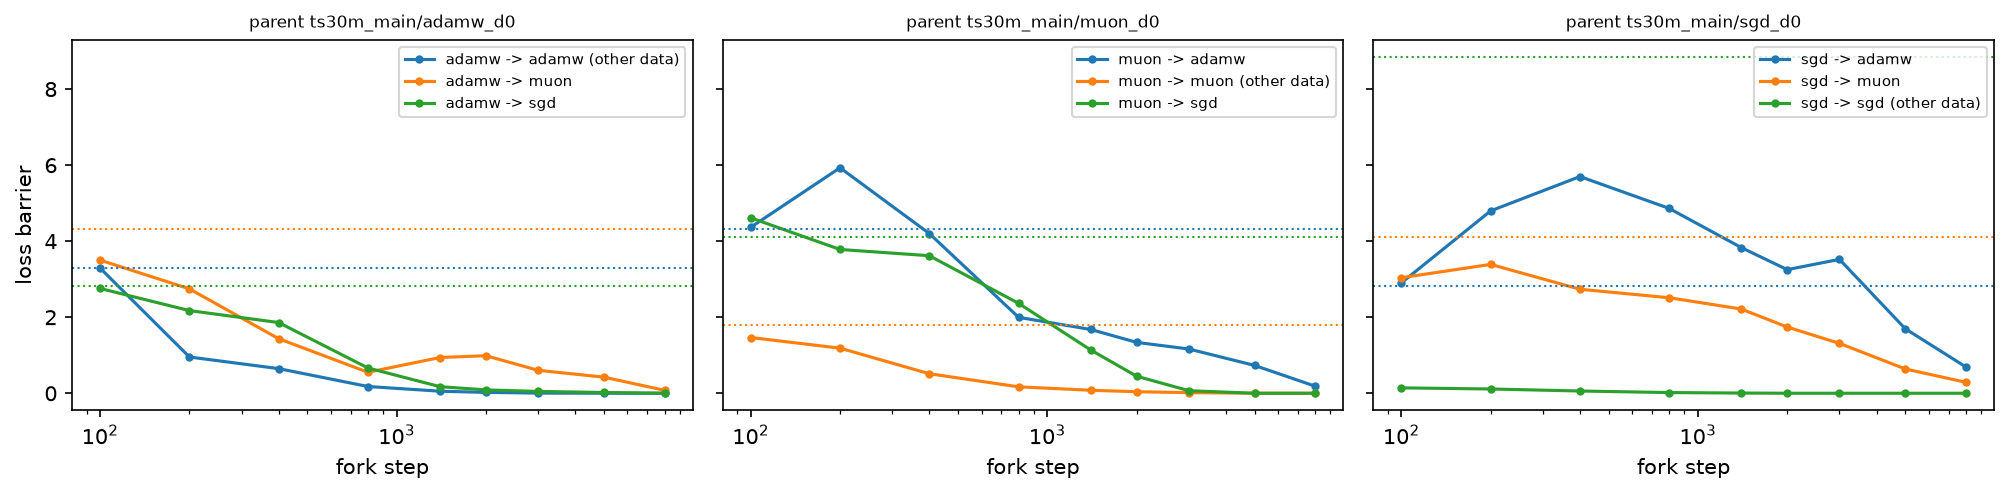
\includegraphics[width=\linewidth]{figures/ts30m/lmc.png}
\caption{Swaps (top) and mode connectivity (bottom) on TinyStories-30M, as in \cref{fig:swap}.}
\label{fig:app-swap-30m}
\end{figure}

\begin{figure}[ht]
\centering
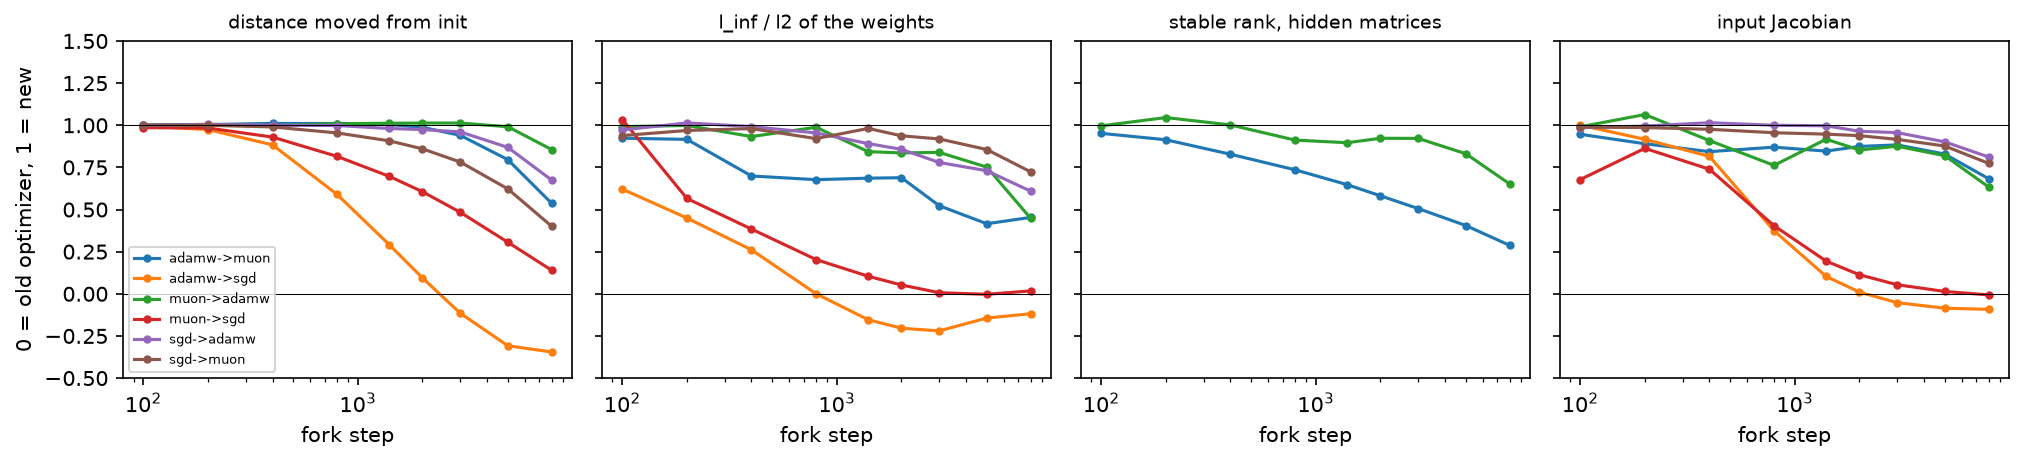
\includegraphics[width=\linewidth]{figures/ts30m/swap_metrics.png}\\[2pt]
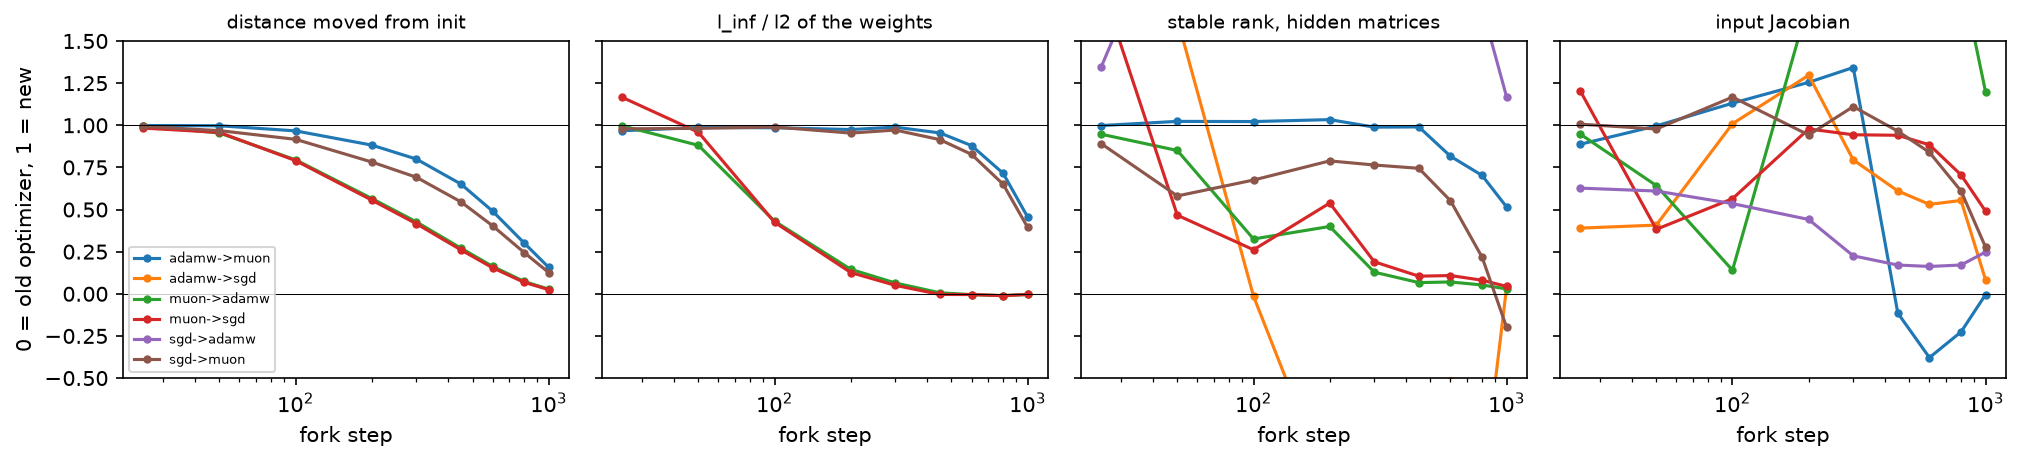
\includegraphics[width=\linewidth]{figures/shakespeare/swap_metrics.png}
\caption{Final metrics of the TinyStories-30M (top) and Shakespeare (bottom) forks between pure A (0) and pure B
(1), as in \cref{fig:swap-metrics}. The stable rank of SGD varies too much over data orders for the pairs with
SGD to show on TinyStories-30M; on Shakespeare SGD's metrics vary widely in general, so most pairs with SGD drop
out or are noisy.}
\label{fig:app-swap-metrics}
\end{figure}

\begin{table}[ht]
\centering\small
\caption{Final function metrics on Shakespeare, mean over the five data orders, as in \cref{tab:metrics}.}
\label{tab:app-metrics-shk}
\begin{tabular}{@{}lrrr@{}}
\toprule
 & SGD & AdamW & Muon \\
\midrule
$\|\theta\|_2$ & 97 & 92 & 654 \\
$\|\theta\|_\infty/\|\theta\|_2$ ($\times10^{3}$) & 12.3 & 12.4 & 2.4 \\
stable rank (hidden, mean) & 63 & 48 & 99 \\
$\|\theta-\theta_0\|/\|\theta_0\|$ & 0.36 & 0.25 & 7.39 \\
input Jacobian (Frobenius) & 46.8 & 120.1 & 162.9 \\
substitution sensitivity & 0.048 & 0.097 & 0.191 \\
top-1 accuracy & 0.323 & 0.554 & 0.533 \\
\bottomrule
\end{tabular}
\end{table}

\begin{figure}[ht]
\centering
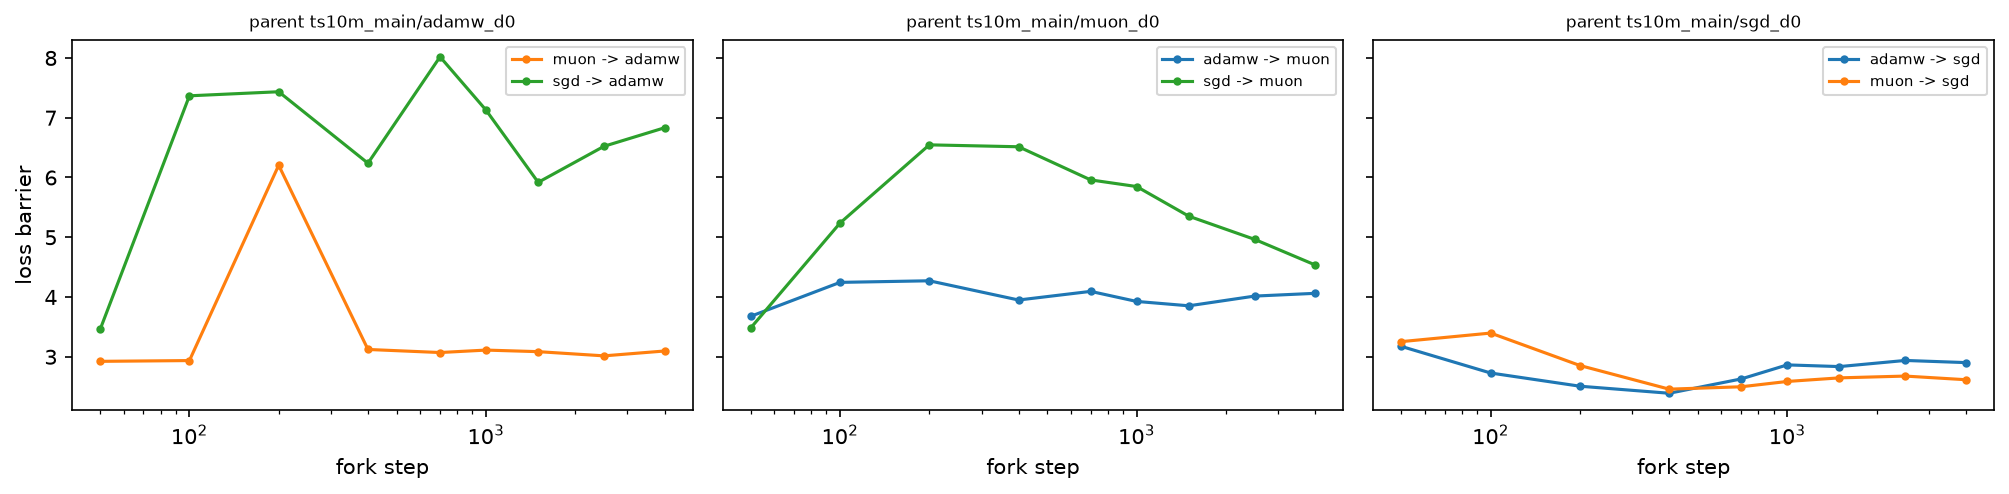
\includegraphics[width=\linewidth]{figures/ts10m/lmc_into.png}\\[2pt]
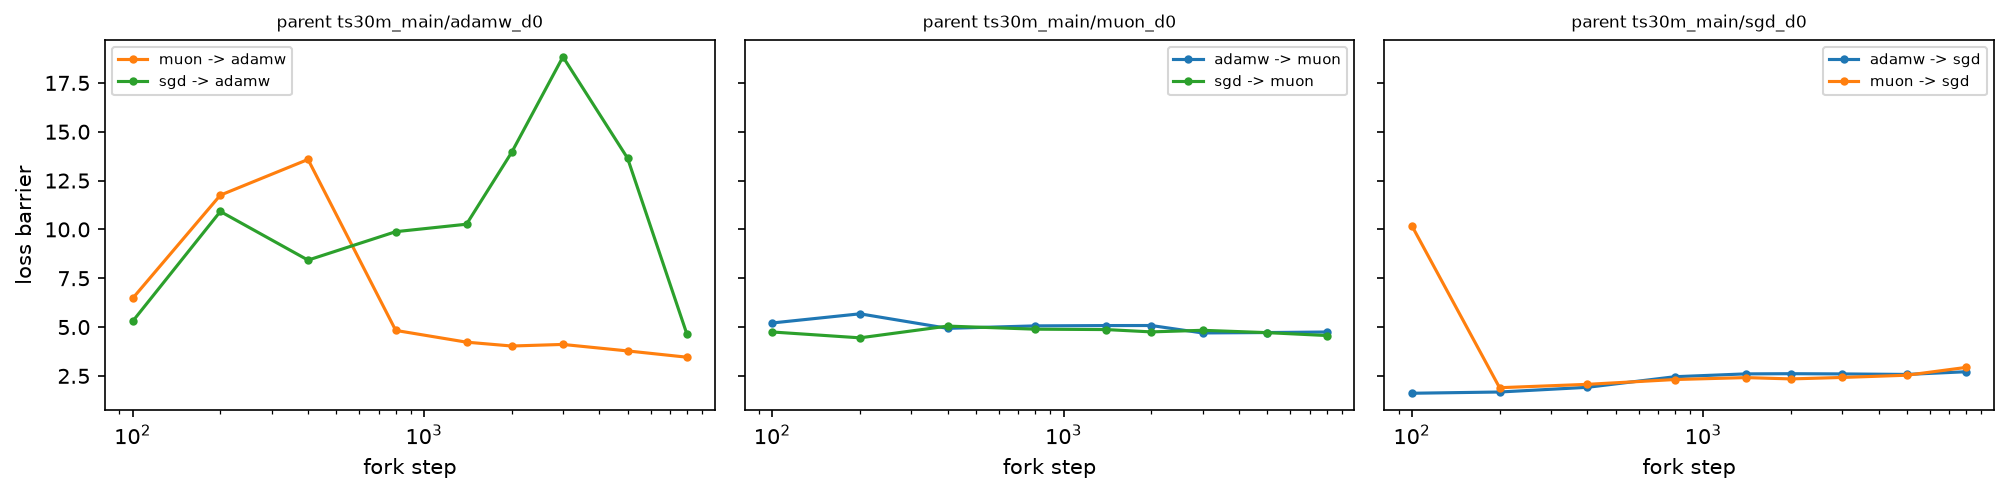
\includegraphics[width=\linewidth]{figures/ts30m/lmc_into.png}\\[2pt]
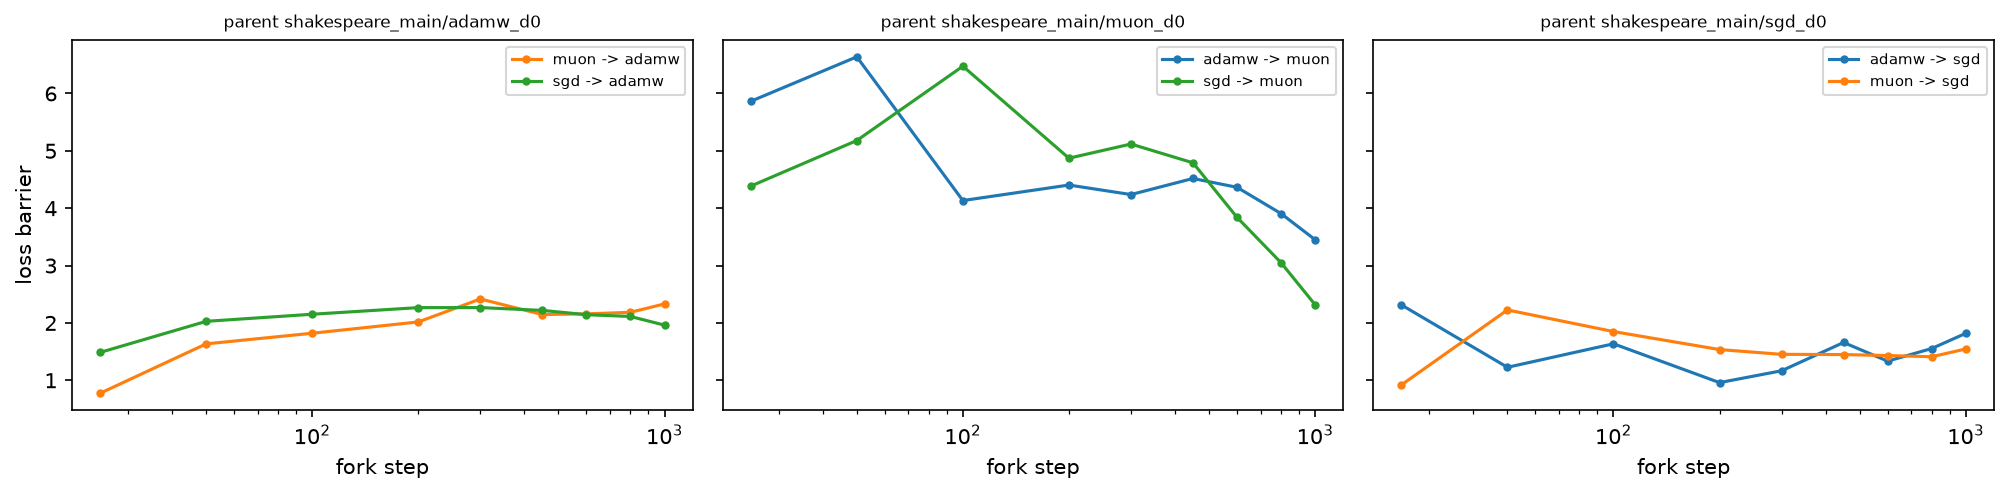
\includegraphics[width=\linewidth]{figures/shakespeare/lmc_into.png}
%% python -m optsplit.analysis.lmc --parent ts10m_main/muon_d0 --forks 'ts10m_forks/*_to_muon_at*' --any-parent --out lmc_into_muon.json
\caption{Barrier between the final weights of each pure $d=0$ run and of every fork into its optimizer, against
the fork step, on TinyStories-10M (top), TinyStories-30M (middle) and Shakespeare (bottom).}
\label{fig:app-lmc-into}
\end{figure}


\end{document}
